\documentclass[twoside]{book}

% Packages required by doxygen
\usepackage{calc}
\usepackage{doxygen}
\usepackage{graphicx}
\usepackage[utf8]{inputenc}
\usepackage{makeidx}
\usepackage{multicol}
\usepackage{multirow}
\usepackage{textcomp}
\usepackage[table]{xcolor}

% Font selection
\usepackage[T1]{fontenc}
\usepackage{mathptmx}
\usepackage[scaled=.90]{helvet}
\usepackage{courier}
\usepackage{amssymb}
\usepackage{sectsty}
\renewcommand{\familydefault}{\sfdefault}
\allsectionsfont{%
  \fontseries{bc}\selectfont%
  \color{darkgray}%
}
\renewcommand{\DoxyLabelFont}{%
  \fontseries{bc}\selectfont%
  \color{darkgray}%
}

% Page & text layout
\usepackage{geometry}
\geometry{%
  a4paper,%
  top=2.5cm,%
  bottom=2.5cm,%
  left=2.5cm,%
  right=2.5cm%
}
\tolerance=750
\hfuzz=15pt
\hbadness=750
\setlength{\emergencystretch}{15pt}
\setlength{\parindent}{0cm}
\setlength{\parskip}{0.2cm}
\makeatletter
\renewcommand{\paragraph}{%
  \@startsection{paragraph}{4}{0ex}{-1.0ex}{1.0ex}{%
    \normalfont\normalsize\bfseries\SS@parafont%
  }%
}
\renewcommand{\subparagraph}{%
  \@startsection{subparagraph}{5}{0ex}{-1.0ex}{1.0ex}{%
    \normalfont\normalsize\bfseries\SS@subparafont%
  }%
}
\makeatother

% Headers & footers
\usepackage{fancyhdr}
\pagestyle{fancyplain}
\fancyhead[LE]{\fancyplain{}{\bfseries\thepage}}
\fancyhead[CE]{\fancyplain{}{}}
\fancyhead[RE]{\fancyplain{}{\bfseries\leftmark}}
\fancyhead[LO]{\fancyplain{}{\bfseries\rightmark}}
\fancyhead[CO]{\fancyplain{}{}}
\fancyhead[RO]{\fancyplain{}{\bfseries\thepage}}
\fancyfoot[LE]{\fancyplain{}{}}
\fancyfoot[CE]{\fancyplain{}{}}
\fancyfoot[RE]{\fancyplain{}{\bfseries\scriptsize Generated on Sat Sep 26 2015 13\-:25\-:56 for Pangea World Generator by Doxygen }}
\fancyfoot[LO]{\fancyplain{}{\bfseries\scriptsize Generated on Sat Sep 26 2015 13\-:25\-:56 for Pangea World Generator by Doxygen }}
\fancyfoot[CO]{\fancyplain{}{}}
\fancyfoot[RO]{\fancyplain{}{}}
\renewcommand{\footrulewidth}{0.4pt}
\renewcommand{\chaptermark}[1]{%
  \markboth{#1}{}%
}
\renewcommand{\sectionmark}[1]{%
  \markright{\thesection\ #1}%
}

% Indices & bibliography
\usepackage{natbib}
\usepackage[titles]{tocloft}
\setcounter{tocdepth}{3}
\setcounter{secnumdepth}{5}
\makeindex

% Hyperlinks (required, but should be loaded last)
\usepackage{ifpdf}
\ifpdf
  \usepackage[pdftex,pagebackref=true]{hyperref}
\else
  \usepackage[ps2pdf,pagebackref=true]{hyperref}
\fi
\hypersetup{%
  colorlinks=true,%
  linkcolor=blue,%
  citecolor=blue,%
  unicode%
}

% Custom commands
\newcommand{\clearemptydoublepage}{%
  \newpage{\pagestyle{empty}\cleardoublepage}%
}


%===== C O N T E N T S =====

\begin{document}

% Titlepage & ToC
\hypersetup{pageanchor=false}
\pagenumbering{roman}
\begin{titlepage}
\vspace*{7cm}
\begin{center}%
{\Large Pangea World Generator \\[1ex]\large 0.\-0.\-1 }\\
\vspace*{1cm}
{\large Generated by Doxygen 1.8.6}\\
\vspace*{0.5cm}
{\small Sat Sep 26 2015 13:25:56}\\
\end{center}
\end{titlepage}
\clearemptydoublepage
\tableofcontents
\clearemptydoublepage
\pagenumbering{arabic}
\hypersetup{pageanchor=true}

%--- Begin generated contents ---
\chapter{Todo List}
\label{todo}
\hypertarget{todo}{}

\begin{DoxyRefList}
\item[\label{todo__todo000001}%
\hypertarget{todo__todo000001}{}%
Global \hyperlink{class_window_entity_a1574c223b3dab59a901b7f4f2fce95c1}{Window\-Entity\-:\-:load\-From\-Instructions} (std\-::string instruction\-String)]Interpréter les strings comme des entiers pour priority 
\end{DoxyRefList}
\chapter{Namespace Index}
\section{Namespace List}
Here is a list of all namespaces with brief descriptions\-:\begin{DoxyCompactList}
\item\contentsline{section}{\hyperlink{namespace_uchronia}{Uchronia} }{\pageref{namespace_uchronia}}{}
\item\contentsline{section}{\hyperlink{namespace_unoise}{Unoise} \\*\hyperlink{namespace_uchronia}{Uchronia} noise namespace }{\pageref{namespace_unoise}}{}
\end{DoxyCompactList}

\chapter{Hierarchical Index}
\section{Class Hierarchy}
This inheritance list is sorted roughly, but not completely, alphabetically\-:\begin{DoxyCompactList}
\item Clock\begin{DoxyCompactList}
\item \contentsline{section}{Timer}{\pageref{class_timer}}{}
\end{DoxyCompactList}
\item \contentsline{section}{Unoise\-:\-:Diamond\-Perm\-Table}{\pageref{struct_unoise_1_1_diamond_perm_table}}{}
\item \contentsline{section}{Main\-U\-I}{\pageref{class_main_u_i}}{}
\item \contentsline{section}{Ntsa\-Window}{\pageref{class_ntsa_window}}{}
\item \contentsline{section}{Unoise\-:\-:point2\-Dui}{\pageref{struct_unoise_1_1point2_dui}}{}
\item \contentsline{section}{Public\-Rect}{\pageref{class_public_rect}}{}
\item \contentsline{section}{Rect}{\pageref{class_rect}}{}
\begin{DoxyCompactList}
\item \contentsline{section}{Window\-Entity}{\pageref{class_window_entity}}{}
\begin{DoxyCompactList}
\item \contentsline{section}{Button}{\pageref{class_button}}{}
\item \contentsline{section}{Entity}{\pageref{class_entity}}{}
\begin{DoxyCompactList}
\item \contentsline{section}{Player}{\pageref{class_player}}{}
\end{DoxyCompactList}
\item \contentsline{section}{Visual\-Effect}{\pageref{class_visual_effect}}{}
\begin{DoxyCompactList}
\item \contentsline{section}{Space\-Laser}{\pageref{class_space_laser}}{}
\end{DoxyCompactList}
\end{DoxyCompactList}
\end{DoxyCompactList}
\item \contentsline{section}{Sprite\-List}{\pageref{class_sprite_list}}{}
\item \contentsline{section}{Texture\-List}{\pageref{class_texture_list}}{}
\end{DoxyCompactList}

\chapter{Data Structure Index}
\section{Data Structures}
Here are the data structures with brief descriptions\-:\begin{DoxyCompactList}
\item\contentsline{section}{\hyperlink{class_button}{Button} \\*Simple U\-I element that does exactly what it mean }{\pageref{class_button}}{}
\item\contentsline{section}{\hyperlink{struct_unoise_1_1_diamond_perm_table}{Unoise\-::\-Diamond\-Perm\-Table} \\*Stock a Perm\-Table \char`\"{}\-Diamond\char`\"{} }{\pageref{struct_unoise_1_1_diamond_perm_table}}{}
\item\contentsline{section}{\hyperlink{class_entity}{Entity} }{\pageref{class_entity}}{}
\item\contentsline{section}{\hyperlink{class_main_u_i}{Main\-U\-I} }{\pageref{class_main_u_i}}{}
\item\contentsline{section}{\hyperlink{class_ntsa_window}{Ntsa\-Window} }{\pageref{class_ntsa_window}}{}
\item\contentsline{section}{\hyperlink{class_player}{Player} }{\pageref{class_player}}{}
\item\contentsline{section}{\hyperlink{struct_unoise_1_1point2_dui}{Unoise\-::point2\-Dui} }{\pageref{struct_unoise_1_1point2_dui}}{}
\item\contentsline{section}{\hyperlink{class_public_rect}{Public\-Rect} }{\pageref{class_public_rect}}{}
\item\contentsline{section}{\hyperlink{class_rect}{Rect} }{\pageref{class_rect}}{}
\item\contentsline{section}{\hyperlink{class_space_laser}{Space\-Laser} \\*Cette classe ressemble en tout points à \hyperlink{class_visual_effect}{Visual\-Effect} mis à part un construxteur légèrement différent }{\pageref{class_space_laser}}{}
\item\contentsline{section}{\hyperlink{class_sprite_list}{Sprite\-List} }{\pageref{class_sprite_list}}{}
\item\contentsline{section}{\hyperlink{class_texture_list}{Texture\-List} }{\pageref{class_texture_list}}{}
\item\contentsline{section}{\hyperlink{class_timer}{Timer} }{\pageref{class_timer}}{}
\item\contentsline{section}{\hyperlink{class_visual_effect}{Visual\-Effect} \\*Une classe gérant effet visuel temporaire }{\pageref{class_visual_effect}}{}
\item\contentsline{section}{\hyperlink{class_window_entity}{Window\-Entity} }{\pageref{class_window_entity}}{}
\end{DoxyCompactList}

\chapter{File Index}
\section{File List}
Here is a list of all files with brief descriptions\-:\begin{DoxyCompactList}
\item\contentsline{section}{src/\hyperlink{_p_world_gen_8cpp}{P\-World\-Gen.\-cpp} }{\pageref{_p_world_gen_8cpp}}{}
\item\contentsline{section}{src/\-Core/\hyperlink{_core_2_u_i_8cpp}{U\-I.\-cpp} }{\pageref{_core_2_u_i_8cpp}}{}
\item\contentsline{section}{src/\-Core/\hyperlink{_core_2_u_i_8h}{U\-I.\-h} }{\pageref{_core_2_u_i_8h}}{}
\item\contentsline{section}{src/\-General/\hyperlink{general_8cpp}{general.\-cpp} }{\pageref{general_8cpp}}{}
\item\contentsline{section}{src/\-General/\hyperlink{general_8h}{general.\-h} }{\pageref{general_8h}}{}
\item\contentsline{section}{src/\-General/\hyperlink{rect_8cpp}{rect.\-cpp} }{\pageref{rect_8cpp}}{}
\item\contentsline{section}{src/\-General/\hyperlink{rect_8h}{rect.\-h} }{\pageref{rect_8h}}{}
\item\contentsline{section}{src/\-General/\hyperlink{usualydefined_8h}{usualydefined.\-h} }{\pageref{usualydefined_8h}}{}
\item\contentsline{section}{src/\-General/\hyperlink{utilities_8cpp}{utilities.\-cpp} }{\pageref{utilities_8cpp}}{}
\item\contentsline{section}{src/\-General/\hyperlink{utilities_8h}{utilities.\-h} }{\pageref{utilities_8h}}{}
\item\contentsline{section}{src/\-Graphics/\hyperlink{entity_8cpp}{entity.\-cpp} }{\pageref{entity_8cpp}}{}
\item\contentsline{section}{src/\-Graphics/\hyperlink{entity_8h}{entity.\-h} }{\pageref{entity_8h}}{}
\item\contentsline{section}{src/\-Graphics/\hyperlink{ntsa_8cpp}{ntsa.\-cpp} }{\pageref{ntsa_8cpp}}{}
\item\contentsline{section}{src/\-Graphics/\hyperlink{ntsa_8h}{ntsa.\-h} }{\pageref{ntsa_8h}}{}
\item\contentsline{section}{src/\-Graphics/\hyperlink{_graphics_2_u_i_8cpp}{U\-I.\-cpp} }{\pageref{_graphics_2_u_i_8cpp}}{}
\item\contentsline{section}{src/\-Graphics/\hyperlink{_graphics_2_u_i_8h}{U\-I.\-h} }{\pageref{_graphics_2_u_i_8h}}{}
\item\contentsline{section}{src/\-Graphics/\hyperlink{_window_entity_8cpp}{Window\-Entity.\-cpp} }{\pageref{_window_entity_8cpp}}{}
\item\contentsline{section}{src/\-Graphics/\hyperlink{_window_entity_8h}{Window\-Entity.\-h} }{\pageref{_window_entity_8h}}{}
\end{DoxyCompactList}

\chapter{Namespace Documentation}
\hypertarget{namespace_uchronia}{\section{Uchronia Namespace Reference}
\label{namespace_uchronia}\index{Uchronia@{Uchronia}}
}

\hypertarget{namespace_unoise}{\section{Unoise Namespace Reference}
\label{namespace_unoise}\index{Unoise@{Unoise}}
}


\hyperlink{namespace_uchronia}{Uchronia} noise namespace.  


\subsection*{Data Structures}
\begin{DoxyCompactItemize}
\item 
struct \hyperlink{struct_unoise_1_1point2_dui}{point2\-Dui}
\item 
struct \hyperlink{struct_unoise_1_1_diamond_perm_table}{Diamond\-Perm\-Table}
\begin{DoxyCompactList}\small\item\em Stock a Perm\-Table \char`\"{}\-Diamond\char`\"{}. \end{DoxyCompactList}\end{DoxyCompactItemize}
\subsection*{Typedefs}
\begin{DoxyCompactItemize}
\item 
typedef std\-::array$<$ unsigned \\*
short, 256 $>$ \hyperlink{namespace_unoise_ae11142038f2dd1bea2711b2b99bbfaf6}{Perm\-Table}
\item 
typedef std\-::vector\\*
$<$ std\-::vector$<$ float $>$ $>$ \hyperlink{namespace_unoise_ac1e5c6227ab68e4e8c1ad57fdbddf51b}{Chunk\-Points}
\end{DoxyCompactItemize}
\subsection*{Functions}
\begin{DoxyCompactItemize}
\item 
void \hyperlink{namespace_unoise_a5dbbb2ae6c75efd29abd5663db08ec0e}{set\-Seed} (int graine)
\item 
void \hyperlink{namespace_unoise_aa8daebdaad2fc5a125cd7b1acc7a38b4}{set\-Perm\-Table} (\hyperlink{namespace_unoise_ae11142038f2dd1bea2711b2b99bbfaf6}{Perm\-Table} $\ast$perm)
\begin{DoxyCompactList}\small\item\em Pas obligatoire, cette fonction permet de changer lambda\-Perm\-Table. \end{DoxyCompactList}\item 
void \hyperlink{namespace_unoise_a5a1dbb7caee818c615fdfedc2ff19730}{gen\-Perm\-Table} (\hyperlink{namespace_unoise_ae11142038f2dd1bea2711b2b99bbfaf6}{Perm\-Table} $\ast$, int)
\begin{DoxyCompactList}\small\item\em On génère la table de permutation à partir d'un seed. \end{DoxyCompactList}\item 
std\-::vector$<$ float $>$ \hyperlink{namespace_unoise_aa685d2a385bbfe1a71a1650004238202}{get\-Positions\-Around} (\hyperlink{namespace_unoise_ac1e5c6227ab68e4e8c1ad57fdbddf51b}{Chunk\-Points} $\ast$tableau, \hyperlink{struct_unoise_1_1point2_dui}{point2\-Dui} point, int pas, std\-::array$<$ std\-::vector$<$ float $>$, 4 $>$ $\ast$points\-Environnants=nullptr, bool phase=1)
\item 
\hyperlink{namespace_unoise_ac1e5c6227ab68e4e8c1ad57fdbddf51b}{Chunk\-Points} \hyperlink{namespace_unoise_accabbc2fce05f7a55bd10ec573925275}{diamond\-Square\-Noise} (float x, float y, int amplitude, float res, unsigned short sub\-Divisions, int nseed=-\/1, std\-::array$<$ float, 4 $>$ $\ast$points\-Principaux=nullptr, std\-::array$<$ std\-::vector$<$ float $>$, 4 $>$ $\ast$points\-Environnants=nullptr)
\begin{DoxyCompactList}\small\item\em Midpoint displacement noise, ou Diamond square noise (nom latin\-: carrus diamus) \end{DoxyCompactList}\item 
float \hyperlink{namespace_unoise_a77b87fa88183eb7081d3ea602989c59e}{perlin\-Noise} (float x, float z, float res, \hyperlink{namespace_unoise_ae11142038f2dd1bea2711b2b99bbfaf6}{Perm\-Table} $\ast$perm=nullptr)
\begin{DoxyCompactList}\small\item\em Fonction du bruit de perlin (float x, float z, float resolution, table de permutation)\-: \end{DoxyCompactList}\end{DoxyCompactItemize}
\subsection*{Variables}
\begin{DoxyCompactItemize}
\item 
\hyperlink{namespace_unoise_ae11142038f2dd1bea2711b2b99bbfaf6}{Perm\-Table} $\ast$ \hyperlink{namespace_unoise_acf4515c07424188371eeb9cf77d34fb3}{lambda\-Perm\-Table} =nullptr
\item 
int \hyperlink{namespace_unoise_ae6356ffd0fec247f6d19c762e1757fc3}{seed} =42
\end{DoxyCompactItemize}


\subsection{Detailed Description}
\hyperlink{namespace_uchronia}{Uchronia} noise namespace. 

\subsection{Typedef Documentation}
\hypertarget{namespace_unoise_ac1e5c6227ab68e4e8c1ad57fdbddf51b}{\index{Unoise@{Unoise}!Chunk\-Points@{Chunk\-Points}}
\index{Chunk\-Points@{Chunk\-Points}!Unoise@{Unoise}}
\subsubsection[{Chunk\-Points}]{\setlength{\rightskip}{0pt plus 5cm}typedef std\-::vector$<$std\-::vector$<$float$>$ $>$ {\bf Unoise\-::\-Chunk\-Points}}}\label{namespace_unoise_ac1e5c6227ab68e4e8c1ad57fdbddf51b}


Definition at line 100 of file utilities.\-h.

\hypertarget{namespace_unoise_ae11142038f2dd1bea2711b2b99bbfaf6}{\index{Unoise@{Unoise}!Perm\-Table@{Perm\-Table}}
\index{Perm\-Table@{Perm\-Table}!Unoise@{Unoise}}
\subsubsection[{Perm\-Table}]{\setlength{\rightskip}{0pt plus 5cm}typedef std\-::array$<$unsigned short, 256$>$ {\bf Unoise\-::\-Perm\-Table}}}\label{namespace_unoise_ae11142038f2dd1bea2711b2b99bbfaf6}


Definition at line 99 of file utilities.\-h.



\subsection{Function Documentation}
\hypertarget{namespace_unoise_accabbc2fce05f7a55bd10ec573925275}{\index{Unoise@{Unoise}!diamond\-Square\-Noise@{diamond\-Square\-Noise}}
\index{diamond\-Square\-Noise@{diamond\-Square\-Noise}!Unoise@{Unoise}}
\subsubsection[{diamond\-Square\-Noise}]{\setlength{\rightskip}{0pt plus 5cm}{\bf Chunk\-Points} Unoise\-::diamond\-Square\-Noise (
\begin{DoxyParamCaption}
\item[{float}]{x, }
\item[{float}]{y, }
\item[{int}]{amplitude, }
\item[{float}]{res, }
\item[{{\bf ushort}}]{sub\-Divisions, }
\item[{int}]{nseed, }
\item[{std\-::array$<$ float, 4 $>$ $\ast$}]{points\-Principaux, }
\item[{std\-::array$<$ std\-::vector$<$ float $>$, 4 $>$ $\ast$}]{points\-Environnants}
\end{DoxyParamCaption}
)}}\label{namespace_unoise_accabbc2fce05f7a55bd10ec573925275}


Midpoint displacement noise, ou Diamond square noise (nom latin\-: carrus diamus) 

Cet algo génère sur une zone memoire donnée un bruit de type midpoint displacement \begin{DoxyNote}{Note}
Vous trouverez des informations sur le fonctionnement interne de cette fonction dans le fichier algoinfos rubrique diamond\-Square\-Noise 
\end{DoxyNote}
\begin{DoxyWarning}{Warning}
Il est interdit de mettre pos à 1 ou à 0, car ça signifierait que le nombre de point par coté vaut 2 
\end{DoxyWarning}

\begin{DoxyParams}{Parameters}
{\em x} & La position du chunk virtuelle X, inutile dans les versions primitives de la fonction \\
\hline
{\em y} & La position du chunk virtuelle Y, inutile dans les versions primitives de la fonction \\
\hline
{\em amplitude} & La hauteur maximale d'un point (la valeur minimale est l'opposée de l'amplitude \\
\hline
{\em res} & La résolution, c'est à dire la rapidité de la réduction du bruit \\
\hline
{\em sub\-Divisions} & Le nombre de subdivisions appliqués, pour trouver le nombre de points par coté ça fait, calculez\-: pow(2, sub\-Divisions)+1 \\
\hline
\end{DoxyParams}


Definition at line 232 of file utilities.\-cpp.



Here is the call graph for this function\-:\nopagebreak
\begin{figure}[H]
\begin{center}
\leavevmode
\includegraphics[width=350pt]{namespace_unoise_accabbc2fce05f7a55bd10ec573925275_cgraph}
\end{center}
\end{figure}


\hypertarget{namespace_unoise_a5a1dbb7caee818c615fdfedc2ff19730}{\index{Unoise@{Unoise}!gen\-Perm\-Table@{gen\-Perm\-Table}}
\index{gen\-Perm\-Table@{gen\-Perm\-Table}!Unoise@{Unoise}}
\subsubsection[{gen\-Perm\-Table}]{\setlength{\rightskip}{0pt plus 5cm}void Unoise\-::gen\-Perm\-Table (
\begin{DoxyParamCaption}
\item[{Perm\-Table $\ast$}]{pttable, }
\item[{int}]{seed}
\end{DoxyParamCaption}
)}}\label{namespace_unoise_a5a1dbb7caee818c615fdfedc2ff19730}


On génère la table de permutation à partir d'un seed. 


\begin{DoxyParams}{Parameters}
{\em pttable} & pointeur via une table de permutation qui sera générée avec le seed \\
\hline
{\em seed} & le seed \\
\hline
\end{DoxyParams}


Definition at line 130 of file utilities.\-cpp.



Referenced by perlin\-Noise().



Here is the call graph for this function\-:\nopagebreak
\begin{figure}[H]
\begin{center}
\leavevmode
\includegraphics[width=322pt]{namespace_unoise_a5a1dbb7caee818c615fdfedc2ff19730_cgraph}
\end{center}
\end{figure}


\hypertarget{namespace_unoise_aa685d2a385bbfe1a71a1650004238202}{\index{Unoise@{Unoise}!get\-Positions\-Around@{get\-Positions\-Around}}
\index{get\-Positions\-Around@{get\-Positions\-Around}!Unoise@{Unoise}}
\subsubsection[{get\-Positions\-Around}]{\setlength{\rightskip}{0pt plus 5cm}std\-::vector$<$float$>$ Unoise\-::get\-Positions\-Around (
\begin{DoxyParamCaption}
\item[{Chunk\-Points $\ast$}]{tableau, }
\item[{point2\-Dui}]{point, }
\item[{int}]{pas, }
\item[{std\-::array$<$ std\-::vector$<$ float $>$, 4 $>$ $\ast$}]{points\-Environnants = {\ttfamily nullptr}, }
\item[{bool}]{phase = {\ttfamily 1}}
\end{DoxyParamCaption}
)}}\label{namespace_unoise_aa685d2a385bbfe1a71a1650004238202}
Cette fonction va donner à l'utilisateur la hauteur des quatres points les plus proches \begin{DoxyNote}{Note}
Elle n'est faite que pour être utilisée par Diamond\-Square\-Noise 
\end{DoxyNote}
\begin{DoxyWarning}{Warning}
Si cette fonction occure un segfault, celà vient probablement du fait que pas ou tableau est à une valeur érronnée 
\end{DoxyWarning}

\begin{DoxyParams}{Parameters}
{\em tableau} & Une référence vers le chunk père du point \\
\hline
{\em pas} & Le nombre de points par lequel on est autorisé à parcourir le chunk (de un \par
 en un pour les chunk finis, de quatre en quatre pour les chunks qu'il reste à subdiviser deux fois) \\
\hline
{\em phase} & Détermine si le point est en phase carré ou diamond, ce qui nous donne un indice sur les points l'environnant \\
\hline
\end{DoxyParams}


Definition at line 171 of file utilities.\-cpp.



Referenced by diamond\-Square\-Noise().

\hypertarget{namespace_unoise_a77b87fa88183eb7081d3ea602989c59e}{\index{Unoise@{Unoise}!perlin\-Noise@{perlin\-Noise}}
\index{perlin\-Noise@{perlin\-Noise}!Unoise@{Unoise}}
\subsubsection[{perlin\-Noise}]{\setlength{\rightskip}{0pt plus 5cm}float Unoise\-::perlin\-Noise (
\begin{DoxyParamCaption}
\item[{float}]{x, }
\item[{float}]{y, }
\item[{float}]{res, }
\item[{Perm\-Table $\ast$}]{perm}
\end{DoxyParamCaption}
)}}\label{namespace_unoise_a77b87fa88183eb7081d3ea602989c59e}


Fonction du bruit de perlin (float x, float z, float resolution, table de permutation)\-: 


\begin{DoxyParams}{Parameters}
{\em x} & La position X \\
\hline
{\em y} & La position Z \\
\hline
{\em res} & La douceur du terrain \\
\hline
{\em perm} & Le pointeur vers la table de permutation \\
\hline
\end{DoxyParams}
\begin{DoxyWarning}{Warning}
La fonction est défective 
\end{DoxyWarning}


Definition at line 322 of file utilities.\-cpp.



Here is the call graph for this function\-:\nopagebreak
\begin{figure}[H]
\begin{center}
\leavevmode
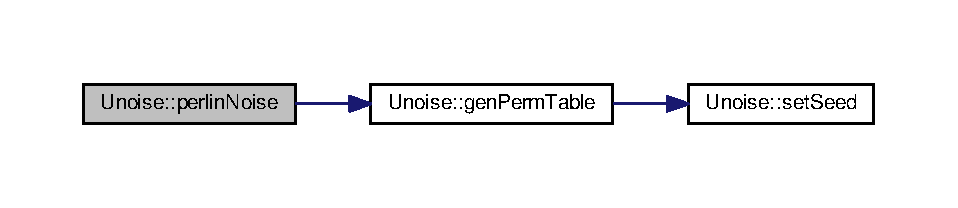
\includegraphics[width=350pt]{namespace_unoise_a77b87fa88183eb7081d3ea602989c59e_cgraph}
\end{center}
\end{figure}


\hypertarget{namespace_unoise_aa8daebdaad2fc5a125cd7b1acc7a38b4}{\index{Unoise@{Unoise}!set\-Perm\-Table@{set\-Perm\-Table}}
\index{set\-Perm\-Table@{set\-Perm\-Table}!Unoise@{Unoise}}
\subsubsection[{set\-Perm\-Table}]{\setlength{\rightskip}{0pt plus 5cm}void Unoise\-::set\-Perm\-Table (
\begin{DoxyParamCaption}
\item[{Perm\-Table $\ast$}]{perm}
\end{DoxyParamCaption}
)}}\label{namespace_unoise_aa8daebdaad2fc5a125cd7b1acc7a38b4}


Pas obligatoire, cette fonction permet de changer lambda\-Perm\-Table. 



Definition at line 124 of file utilities.\-cpp.

\hypertarget{namespace_unoise_a5dbbb2ae6c75efd29abd5663db08ec0e}{\index{Unoise@{Unoise}!set\-Seed@{set\-Seed}}
\index{set\-Seed@{set\-Seed}!Unoise@{Unoise}}
\subsubsection[{set\-Seed}]{\setlength{\rightskip}{0pt plus 5cm}void Unoise\-::set\-Seed (
\begin{DoxyParamCaption}
\item[{int}]{graine}
\end{DoxyParamCaption}
)}}\label{namespace_unoise_a5dbbb2ae6c75efd29abd5663db08ec0e}


Definition at line 118 of file utilities.\-cpp.



Referenced by gen\-Perm\-Table().



\subsection{Variable Documentation}
\hypertarget{namespace_unoise_acf4515c07424188371eeb9cf77d34fb3}{\index{Unoise@{Unoise}!lambda\-Perm\-Table@{lambda\-Perm\-Table}}
\index{lambda\-Perm\-Table@{lambda\-Perm\-Table}!Unoise@{Unoise}}
\subsubsection[{lambda\-Perm\-Table}]{\setlength{\rightskip}{0pt plus 5cm}{\bf Perm\-Table}$\ast$ Unoise\-::lambda\-Perm\-Table =nullptr}}\label{namespace_unoise_acf4515c07424188371eeb9cf77d34fb3}


Definition at line 115 of file utilities.\-cpp.



Referenced by perlin\-Noise(), and set\-Perm\-Table().

\hypertarget{namespace_unoise_ae6356ffd0fec247f6d19c762e1757fc3}{\index{Unoise@{Unoise}!seed@{seed}}
\index{seed@{seed}!Unoise@{Unoise}}
\subsubsection[{seed}]{\setlength{\rightskip}{0pt plus 5cm}int Unoise\-::seed =42}}\label{namespace_unoise_ae6356ffd0fec247f6d19c762e1757fc3}


Definition at line 116 of file utilities.\-cpp.



Referenced by diamond\-Square\-Noise(), perlin\-Noise(), and set\-Seed().


\chapter{Data Structure Documentation}
\hypertarget{class_button}{\section{Button Class Reference}
\label{class_button}\index{Button@{Button}}
}


The \hyperlink{class_button}{Button} class is a simple U\-I element that does exactly what it mean.  




{\ttfamily \#include $<$U\-I.\-h$>$}



Inheritance diagram for Button\-:\nopagebreak
\begin{figure}[H]
\begin{center}
\leavevmode
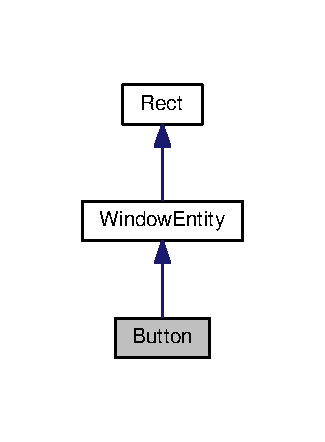
\includegraphics[width=156pt]{class_button__inherit__graph}
\end{center}
\end{figure}


Collaboration diagram for Button\-:\nopagebreak
\begin{figure}[H]
\begin{center}
\leavevmode
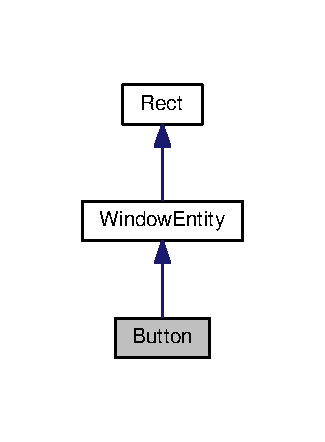
\includegraphics[width=156pt]{class_button__coll__graph}
\end{center}
\end{figure}
\subsection*{Public Member Functions}
\begin{DoxyCompactItemize}
\item 
\hyperlink{class_button_a3b36df1ae23c58aedb9e15a713159459}{Button} ()
\item 
\hyperlink{class_button_a08181944cf12e0e960ba74bdf7cef98e}{Button} (std\-::string name, unsigned int priority, std\-::string texture=\char`\"{}\char`\"{})
\item 
\hyperlink{class_button_ab53e47e7822bd9002eda4f397ffda854}{Button} (std\-::string name, unsigned int priority, float x, float y, float l, float h, std\-::string texture=\char`\"{}\char`\"{})
\item 
bool \hyperlink{class_button_af0c0bca46462e357cd32d007d93d660c}{is\-Pressed} (sf\-::\-Render\-Window $\ast$current\-Window)
\item 
void \hyperlink{class_button_a0d037b742c501f7deb1b4da1a2f3c2a8}{set\-Action} (std\-::string action)
\item 
std\-::string \hyperlink{class_button_a7aafbc7deaf432112e14e9738a2e649a}{get\-Action} ()
\end{DoxyCompactItemize}
\subsection*{Private Attributes}
\begin{DoxyCompactItemize}
\item 
std\-::string \hyperlink{class_button_a2ac72251ae697e3b8f248254d24be694}{m\-\_\-action}
\item 
bool \hyperlink{class_button_a14a55f491951ad95a650bd30111ce1cb}{m\-\_\-pressed} =false
\end{DoxyCompactItemize}
\subsection*{Additional Inherited Members}


\subsection{Detailed Description}
The \hyperlink{class_button}{Button} class is a simple U\-I element that does exactly what it mean. 

Definition at line 8 of file U\-I.\-h.



\subsection{Constructor \& Destructor Documentation}
\hypertarget{class_button_a3b36df1ae23c58aedb9e15a713159459}{\index{Button@{Button}!Button@{Button}}
\index{Button@{Button}!Button@{Button}}
\subsubsection[{Button}]{\setlength{\rightskip}{0pt plus 5cm}Button\-::\-Button (
\begin{DoxyParamCaption}
{}
\end{DoxyParamCaption}
)\hspace{0.3cm}{\ttfamily [inline]}}}\label{class_button_a3b36df1ae23c58aedb9e15a713159459}


Definition at line 11 of file U\-I.\-h.

\hypertarget{class_button_a08181944cf12e0e960ba74bdf7cef98e}{\index{Button@{Button}!Button@{Button}}
\index{Button@{Button}!Button@{Button}}
\subsubsection[{Button}]{\setlength{\rightskip}{0pt plus 5cm}Button\-::\-Button (
\begin{DoxyParamCaption}
\item[{std\-::string}]{name, }
\item[{unsigned int}]{priority, }
\item[{std\-::string}]{texture = {\ttfamily \char`\"{}\char`\"{}}}
\end{DoxyParamCaption}
)}}\label{class_button_a08181944cf12e0e960ba74bdf7cef98e}


Definition at line 3 of file U\-I.\-cpp.

\hypertarget{class_button_ab53e47e7822bd9002eda4f397ffda854}{\index{Button@{Button}!Button@{Button}}
\index{Button@{Button}!Button@{Button}}
\subsubsection[{Button}]{\setlength{\rightskip}{0pt plus 5cm}Button\-::\-Button (
\begin{DoxyParamCaption}
\item[{std\-::string}]{name, }
\item[{unsigned int}]{priority, }
\item[{float}]{x, }
\item[{float}]{y, }
\item[{float}]{l, }
\item[{float}]{h, }
\item[{std\-::string}]{texture = {\ttfamily \char`\"{}\char`\"{}}}
\end{DoxyParamCaption}
)}}\label{class_button_ab53e47e7822bd9002eda4f397ffda854}


Definition at line 7 of file U\-I.\-cpp.



Here is the call graph for this function\-:\nopagebreak
\begin{figure}[H]
\begin{center}
\leavevmode
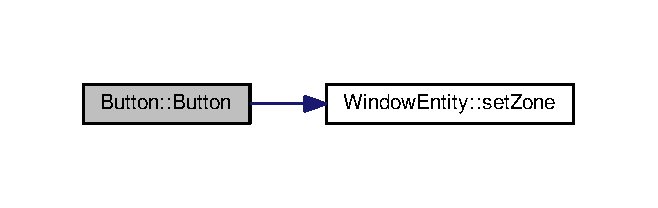
\includegraphics[width=316pt]{class_button_ab53e47e7822bd9002eda4f397ffda854_cgraph}
\end{center}
\end{figure}




\subsection{Member Function Documentation}
\hypertarget{class_button_a7aafbc7deaf432112e14e9738a2e649a}{\index{Button@{Button}!get\-Action@{get\-Action}}
\index{get\-Action@{get\-Action}!Button@{Button}}
\subsubsection[{get\-Action}]{\setlength{\rightskip}{0pt plus 5cm}std\-::string Button\-::get\-Action (
\begin{DoxyParamCaption}
{}
\end{DoxyParamCaption}
)\hspace{0.3cm}{\ttfamily [inline]}}}\label{class_button_a7aafbc7deaf432112e14e9738a2e649a}


Definition at line 20 of file U\-I.\-h.

\hypertarget{class_button_af0c0bca46462e357cd32d007d93d660c}{\index{Button@{Button}!is\-Pressed@{is\-Pressed}}
\index{is\-Pressed@{is\-Pressed}!Button@{Button}}
\subsubsection[{is\-Pressed}]{\setlength{\rightskip}{0pt plus 5cm}bool Button\-::is\-Pressed (
\begin{DoxyParamCaption}
\item[{sf\-::\-Render\-Window $\ast$}]{current\-Window}
\end{DoxyParamCaption}
)}}\label{class_button_af0c0bca46462e357cd32d007d93d660c}


Definition at line 13 of file U\-I.\-cpp.

\hypertarget{class_button_a0d037b742c501f7deb1b4da1a2f3c2a8}{\index{Button@{Button}!set\-Action@{set\-Action}}
\index{set\-Action@{set\-Action}!Button@{Button}}
\subsubsection[{set\-Action}]{\setlength{\rightskip}{0pt plus 5cm}void Button\-::set\-Action (
\begin{DoxyParamCaption}
\item[{std\-::string}]{action}
\end{DoxyParamCaption}
)\hspace{0.3cm}{\ttfamily [inline]}}}\label{class_button_a0d037b742c501f7deb1b4da1a2f3c2a8}


Definition at line 19 of file U\-I.\-h.



\subsection{Field Documentation}
\hypertarget{class_button_a2ac72251ae697e3b8f248254d24be694}{\index{Button@{Button}!m\-\_\-action@{m\-\_\-action}}
\index{m\-\_\-action@{m\-\_\-action}!Button@{Button}}
\subsubsection[{m\-\_\-action}]{\setlength{\rightskip}{0pt plus 5cm}std\-::string Button\-::m\-\_\-action\hspace{0.3cm}{\ttfamily [private]}}}\label{class_button_a2ac72251ae697e3b8f248254d24be694}


Definition at line 20 of file U\-I.\-h.



Referenced by set\-Action().

\hypertarget{class_button_a14a55f491951ad95a650bd30111ce1cb}{\index{Button@{Button}!m\-\_\-pressed@{m\-\_\-pressed}}
\index{m\-\_\-pressed@{m\-\_\-pressed}!Button@{Button}}
\subsubsection[{m\-\_\-pressed}]{\setlength{\rightskip}{0pt plus 5cm}bool Button\-::m\-\_\-pressed =false\hspace{0.3cm}{\ttfamily [private]}}}\label{class_button_a14a55f491951ad95a650bd30111ce1cb}


Definition at line 24 of file U\-I.\-h.



Referenced by is\-Pressed().



The documentation for this class was generated from the following files\-:\begin{DoxyCompactItemize}
\item 
src/\-Graphics/\hyperlink{_graphics_2_u_i_8h}{U\-I.\-h}\item 
src/\-Graphics/\hyperlink{_graphics_2_u_i_8cpp}{U\-I.\-cpp}\end{DoxyCompactItemize}

\hypertarget{struct_unoise_1_1_diamond_perm_table}{\section{Unoise\-:\-:Diamond\-Perm\-Table Struct Reference}
\label{struct_unoise_1_1_diamond_perm_table}\index{Unoise\-::\-Diamond\-Perm\-Table@{Unoise\-::\-Diamond\-Perm\-Table}}
}


Stock a Perm\-Table \char`\"{}\-Diamond\char`\"{}.  




{\ttfamily \#include $<$utilities.\-h$>$}

\subsection*{Data Fields}
\begin{DoxyCompactItemize}
\item 
\hyperlink{namespace_unoise_ae11142038f2dd1bea2711b2b99bbfaf6}{Perm\-Table} \hyperlink{struct_unoise_1_1_diamond_perm_table_abbdd2c631912b46dd642a1742fafc2cc}{perm\-Table}
\item 
\hyperlink{namespace_unoise_ae11142038f2dd1bea2711b2b99bbfaf6}{Perm\-Table} \hyperlink{struct_unoise_1_1_diamond_perm_table_a5445920a0bda0d71a2523175fb125df4}{perm\-Perm\-Table}
\end{DoxyCompactItemize}


\subsection{Detailed Description}
Stock a Perm\-Table \char`\"{}\-Diamond\char`\"{}. 

Definition at line 105 of file utilities.\-h.



\subsection{Field Documentation}
\hypertarget{struct_unoise_1_1_diamond_perm_table_a5445920a0bda0d71a2523175fb125df4}{\index{Unoise\-::\-Diamond\-Perm\-Table@{Unoise\-::\-Diamond\-Perm\-Table}!perm\-Perm\-Table@{perm\-Perm\-Table}}
\index{perm\-Perm\-Table@{perm\-Perm\-Table}!Unoise::DiamondPermTable@{Unoise\-::\-Diamond\-Perm\-Table}}
\subsubsection[{perm\-Perm\-Table}]{\setlength{\rightskip}{0pt plus 5cm}{\bf Perm\-Table} Unoise\-::\-Diamond\-Perm\-Table\-::perm\-Perm\-Table}}\label{struct_unoise_1_1_diamond_perm_table_a5445920a0bda0d71a2523175fb125df4}


Definition at line 108 of file utilities.\-h.

\hypertarget{struct_unoise_1_1_diamond_perm_table_abbdd2c631912b46dd642a1742fafc2cc}{\index{Unoise\-::\-Diamond\-Perm\-Table@{Unoise\-::\-Diamond\-Perm\-Table}!perm\-Table@{perm\-Table}}
\index{perm\-Table@{perm\-Table}!Unoise::DiamondPermTable@{Unoise\-::\-Diamond\-Perm\-Table}}
\subsubsection[{perm\-Table}]{\setlength{\rightskip}{0pt plus 5cm}{\bf Perm\-Table} Unoise\-::\-Diamond\-Perm\-Table\-::perm\-Table}}\label{struct_unoise_1_1_diamond_perm_table_abbdd2c631912b46dd642a1742fafc2cc}


Definition at line 107 of file utilities.\-h.



The documentation for this struct was generated from the following file\-:\begin{DoxyCompactItemize}
\item 
src/\-General/\hyperlink{utilities_8h}{utilities.\-h}\end{DoxyCompactItemize}

\hypertarget{class_entity}{\section{Entity Class Reference}
\label{class_entity}\index{Entity@{Entity}}
}


{\ttfamily \#include $<$entity.\-h$>$}



Inheritance diagram for Entity\-:\nopagebreak
\begin{figure}[H]
\begin{center}
\leavevmode
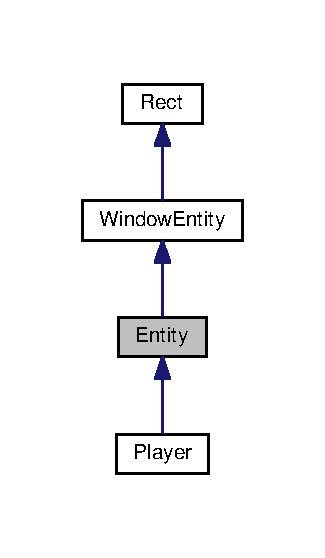
\includegraphics[width=156pt]{class_entity__inherit__graph}
\end{center}
\end{figure}


Collaboration diagram for Entity\-:\nopagebreak
\begin{figure}[H]
\begin{center}
\leavevmode
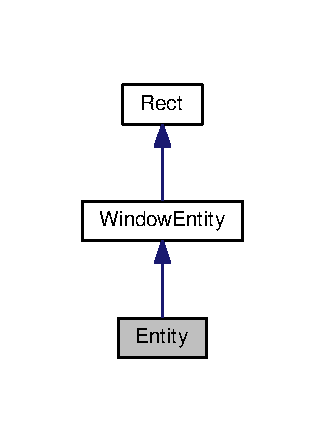
\includegraphics[width=156pt]{class_entity__coll__graph}
\end{center}
\end{figure}
\subsection*{Public Types}
\begin{DoxyCompactItemize}
\item 
enum \hyperlink{class_entity_ac6ff3a9435d7dacb378891eadd127034}{Direction} \{ \\*
\hyperlink{class_entity_ac6ff3a9435d7dacb378891eadd127034a4803b5fc09325c357306efca6aec7d51}{Up}, 
\hyperlink{class_entity_ac6ff3a9435d7dacb378891eadd127034aca17a432012ff0ad12d64fb7002a8dfb}{Down}, 
\hyperlink{class_entity_ac6ff3a9435d7dacb378891eadd127034acdaf97e899d1e2f8c6e954407b9e9639}{Front}, 
\hyperlink{class_entity_ac6ff3a9435d7dacb378891eadd127034a8c4d4b4ceef8bff2884d0bf450a0bff6}{Back}, 
\\*
\hyperlink{class_entity_ac6ff3a9435d7dacb378891eadd127034a869b7581994c699f0dab2b617d30a12d}{Nope}
 \}
\end{DoxyCompactItemize}
\subsection*{Public Member Functions}
\begin{DoxyCompactItemize}
\item 
\hyperlink{class_entity_a980f368aa07ce358583982821533a54a}{Entity} ()
\item 
\hyperlink{class_entity_af0d855b4b36ea55fa5e374e3381c13cc}{Entity} (std\-::string name, unsigned int priority, std\-::string texture\-I\-D=\char`\"{}\char`\"{})
\item 
void \hyperlink{class_entity_a2e553246efacb426f0806faf59b017e7}{stabilize} ()
\item 
void \hyperlink{class_entity_a7c921a26a91394a2cb6aca2aae78bbbe}{stop\-Moving} ()
\item 
void \hyperlink{class_entity_a4b8c151c2e5f7337b4cf74df6ccc62f5}{stop\-Acceleration} ()
\item 
void \hyperlink{class_entity_a0f563cb7a800d95e7b8f2c030f9435f4}{move\-Somewere} (\hyperlink{class_entity_ac6ff3a9435d7dacb378891eadd127034}{Direction} direction)
\end{DoxyCompactItemize}
\subsection*{Protected Member Functions}
\begin{DoxyCompactItemize}
\item 
void \hyperlink{class_entity_aba5b0aae47c86e29e813d91e9bcab02b}{set\-Speed\-Up\-Down} (int speed=3)
\item 
void \hyperlink{class_entity_a5f6cf81a507a7b4a4068528b3c9faf24}{set\-Speed\-Front} (int speed=4)
\end{DoxyCompactItemize}
\subsection*{Protected Attributes}
\begin{DoxyCompactItemize}
\item 
float \hyperlink{class_entity_aee87de23c1e63a14dff1f2dd8597496d}{m\-\_\-speed\-Up\-Down} =0
\item 
float \hyperlink{class_entity_a6355c1ec7f08c88b955c7960b8e1ef60}{m\-\_\-speed\-Front} =0
\item 
unsigned int \hyperlink{class_entity_aeffb6deae5015518100f49b680a44fa0}{m\-\_\-life\-Points} =100
\item 
\hyperlink{class_entity_ac6ff3a9435d7dacb378891eadd127034}{Direction} \hyperlink{class_entity_a687d37b15315f2b663f1b63576281bd2}{m\-\_\-direction\-Acceleration} =Direction\-::\-Nope
\end{DoxyCompactItemize}


\subsection{Detailed Description}
Classiquement, une entité représente un élément du niveau qui peut se mouvoir (un ennemi, où même un simple astéroide de passage) \par
mais également intéragir avec les autres entités via les collisions 

Definition at line 17 of file entity.\-h.



\subsection{Member Enumeration Documentation}
\hypertarget{class_entity_ac6ff3a9435d7dacb378891eadd127034}{\index{Entity@{Entity}!Direction@{Direction}}
\index{Direction@{Direction}!Entity@{Entity}}
\subsubsection[{Direction}]{\setlength{\rightskip}{0pt plus 5cm}enum {\bf Entity\-::\-Direction}}}\label{class_entity_ac6ff3a9435d7dacb378891eadd127034}
\begin{Desc}
\item[Enumerator]\par
\begin{description}
\index{Up@{Up}!Entity@{Entity}}\index{Entity@{Entity}!Up@{Up}}\item[{\em 
\hypertarget{class_entity_ac6ff3a9435d7dacb378891eadd127034a4803b5fc09325c357306efca6aec7d51}{Up}\label{class_entity_ac6ff3a9435d7dacb378891eadd127034a4803b5fc09325c357306efca6aec7d51}
}]\index{Down@{Down}!Entity@{Entity}}\index{Entity@{Entity}!Down@{Down}}\item[{\em 
\hypertarget{class_entity_ac6ff3a9435d7dacb378891eadd127034aca17a432012ff0ad12d64fb7002a8dfb}{Down}\label{class_entity_ac6ff3a9435d7dacb378891eadd127034aca17a432012ff0ad12d64fb7002a8dfb}
}]\index{Front@{Front}!Entity@{Entity}}\index{Entity@{Entity}!Front@{Front}}\item[{\em 
\hypertarget{class_entity_ac6ff3a9435d7dacb378891eadd127034acdaf97e899d1e2f8c6e954407b9e9639}{Front}\label{class_entity_ac6ff3a9435d7dacb378891eadd127034acdaf97e899d1e2f8c6e954407b9e9639}
}]\index{Back@{Back}!Entity@{Entity}}\index{Entity@{Entity}!Back@{Back}}\item[{\em 
\hypertarget{class_entity_ac6ff3a9435d7dacb378891eadd127034a8c4d4b4ceef8bff2884d0bf450a0bff6}{Back}\label{class_entity_ac6ff3a9435d7dacb378891eadd127034a8c4d4b4ceef8bff2884d0bf450a0bff6}
}]\index{Nope@{Nope}!Entity@{Entity}}\index{Entity@{Entity}!Nope@{Nope}}\item[{\em 
\hypertarget{class_entity_ac6ff3a9435d7dacb378891eadd127034a869b7581994c699f0dab2b617d30a12d}{Nope}\label{class_entity_ac6ff3a9435d7dacb378891eadd127034a869b7581994c699f0dab2b617d30a12d}
}]\end{description}
\end{Desc}


Definition at line 20 of file entity.\-h.



\subsection{Constructor \& Destructor Documentation}
\hypertarget{class_entity_a980f368aa07ce358583982821533a54a}{\index{Entity@{Entity}!Entity@{Entity}}
\index{Entity@{Entity}!Entity@{Entity}}
\subsubsection[{Entity}]{\setlength{\rightskip}{0pt plus 5cm}Entity\-::\-Entity (
\begin{DoxyParamCaption}
{}
\end{DoxyParamCaption}
)}}\label{class_entity_a980f368aa07ce358583982821533a54a}


Definition at line 7 of file entity.\-cpp.

\hypertarget{class_entity_af0d855b4b36ea55fa5e374e3381c13cc}{\index{Entity@{Entity}!Entity@{Entity}}
\index{Entity@{Entity}!Entity@{Entity}}
\subsubsection[{Entity}]{\setlength{\rightskip}{0pt plus 5cm}Entity\-::\-Entity (
\begin{DoxyParamCaption}
\item[{std\-::string}]{name, }
\item[{unsigned int}]{priority, }
\item[{std\-::string}]{texture\-I\-D = {\ttfamily \char`\"{}\char`\"{}}}
\end{DoxyParamCaption}
)}}\label{class_entity_af0d855b4b36ea55fa5e374e3381c13cc}


Definition at line 10 of file entity.\-cpp.



\subsection{Member Function Documentation}
\hypertarget{class_entity_a0f563cb7a800d95e7b8f2c030f9435f4}{\index{Entity@{Entity}!move\-Somewere@{move\-Somewere}}
\index{move\-Somewere@{move\-Somewere}!Entity@{Entity}}
\subsubsection[{move\-Somewere}]{\setlength{\rightskip}{0pt plus 5cm}void Entity\-::move\-Somewere (
\begin{DoxyParamCaption}
\item[{{\bf Direction}}]{direction}
\end{DoxyParamCaption}
)}}\label{class_entity_a0f563cb7a800d95e7b8f2c030f9435f4}


Definition at line 30 of file entity.\-cpp.



Referenced by Ntsa\-Window\-::actualize().

\hypertarget{class_entity_a5f6cf81a507a7b4a4068528b3c9faf24}{\index{Entity@{Entity}!set\-Speed\-Front@{set\-Speed\-Front}}
\index{set\-Speed\-Front@{set\-Speed\-Front}!Entity@{Entity}}
\subsubsection[{set\-Speed\-Front}]{\setlength{\rightskip}{0pt plus 5cm}void Entity\-::set\-Speed\-Front (
\begin{DoxyParamCaption}
\item[{int}]{speed = {\ttfamily 4}}
\end{DoxyParamCaption}
)\hspace{0.3cm}{\ttfamily [protected]}}}\label{class_entity_a5f6cf81a507a7b4a4068528b3c9faf24}
\hypertarget{class_entity_aba5b0aae47c86e29e813d91e9bcab02b}{\index{Entity@{Entity}!set\-Speed\-Up\-Down@{set\-Speed\-Up\-Down}}
\index{set\-Speed\-Up\-Down@{set\-Speed\-Up\-Down}!Entity@{Entity}}
\subsubsection[{set\-Speed\-Up\-Down}]{\setlength{\rightskip}{0pt plus 5cm}void Entity\-::set\-Speed\-Up\-Down (
\begin{DoxyParamCaption}
\item[{int}]{speed = {\ttfamily 3}}
\end{DoxyParamCaption}
)\hspace{0.3cm}{\ttfamily [protected]}}}\label{class_entity_aba5b0aae47c86e29e813d91e9bcab02b}
\hypertarget{class_entity_a2e553246efacb426f0806faf59b017e7}{\index{Entity@{Entity}!stabilize@{stabilize}}
\index{stabilize@{stabilize}!Entity@{Entity}}
\subsubsection[{stabilize}]{\setlength{\rightskip}{0pt plus 5cm}void Entity\-::stabilize (
\begin{DoxyParamCaption}
{}
\end{DoxyParamCaption}
)}}\label{class_entity_a2e553246efacb426f0806faf59b017e7}


Definition at line 14 of file entity.\-cpp.



Referenced by Ntsa\-Window\-::actualize().

\hypertarget{class_entity_a4b8c151c2e5f7337b4cf74df6ccc62f5}{\index{Entity@{Entity}!stop\-Acceleration@{stop\-Acceleration}}
\index{stop\-Acceleration@{stop\-Acceleration}!Entity@{Entity}}
\subsubsection[{stop\-Acceleration}]{\setlength{\rightskip}{0pt plus 5cm}void Entity\-::stop\-Acceleration (
\begin{DoxyParamCaption}
{}
\end{DoxyParamCaption}
)}}\label{class_entity_a4b8c151c2e5f7337b4cf74df6ccc62f5}


Definition at line 19 of file entity.\-cpp.



Referenced by Ntsa\-Window\-::actualize().

\hypertarget{class_entity_a7c921a26a91394a2cb6aca2aae78bbbe}{\index{Entity@{Entity}!stop\-Moving@{stop\-Moving}}
\index{stop\-Moving@{stop\-Moving}!Entity@{Entity}}
\subsubsection[{stop\-Moving}]{\setlength{\rightskip}{0pt plus 5cm}void Entity\-::stop\-Moving (
\begin{DoxyParamCaption}
{}
\end{DoxyParamCaption}
)}}\label{class_entity_a7c921a26a91394a2cb6aca2aae78bbbe}


Definition at line 24 of file entity.\-cpp.



\subsection{Field Documentation}
\hypertarget{class_entity_a687d37b15315f2b663f1b63576281bd2}{\index{Entity@{Entity}!m\-\_\-direction\-Acceleration@{m\-\_\-direction\-Acceleration}}
\index{m\-\_\-direction\-Acceleration@{m\-\_\-direction\-Acceleration}!Entity@{Entity}}
\subsubsection[{m\-\_\-direction\-Acceleration}]{\setlength{\rightskip}{0pt plus 5cm}{\bf Direction} Entity\-::m\-\_\-direction\-Acceleration =Direction\-::\-Nope\hspace{0.3cm}{\ttfamily [protected]}}}\label{class_entity_a687d37b15315f2b663f1b63576281bd2}


Definition at line 39 of file entity.\-h.



Referenced by Player\-::actualiser(), move\-Somewere(), and stop\-Acceleration().

\hypertarget{class_entity_aeffb6deae5015518100f49b680a44fa0}{\index{Entity@{Entity}!m\-\_\-life\-Points@{m\-\_\-life\-Points}}
\index{m\-\_\-life\-Points@{m\-\_\-life\-Points}!Entity@{Entity}}
\subsubsection[{m\-\_\-life\-Points}]{\setlength{\rightskip}{0pt plus 5cm}unsigned int Entity\-::m\-\_\-life\-Points =100\hspace{0.3cm}{\ttfamily [protected]}}}\label{class_entity_aeffb6deae5015518100f49b680a44fa0}


Definition at line 34 of file entity.\-h.

\hypertarget{class_entity_a6355c1ec7f08c88b955c7960b8e1ef60}{\index{Entity@{Entity}!m\-\_\-speed\-Front@{m\-\_\-speed\-Front}}
\index{m\-\_\-speed\-Front@{m\-\_\-speed\-Front}!Entity@{Entity}}
\subsubsection[{m\-\_\-speed\-Front}]{\setlength{\rightskip}{0pt plus 5cm}float Entity\-::m\-\_\-speed\-Front =0\hspace{0.3cm}{\ttfamily [protected]}}}\label{class_entity_a6355c1ec7f08c88b955c7960b8e1ef60}


Definition at line 32 of file entity.\-h.



Referenced by stop\-Moving().

\hypertarget{class_entity_aee87de23c1e63a14dff1f2dd8597496d}{\index{Entity@{Entity}!m\-\_\-speed\-Up\-Down@{m\-\_\-speed\-Up\-Down}}
\index{m\-\_\-speed\-Up\-Down@{m\-\_\-speed\-Up\-Down}!Entity@{Entity}}
\subsubsection[{m\-\_\-speed\-Up\-Down}]{\setlength{\rightskip}{0pt plus 5cm}float Entity\-::m\-\_\-speed\-Up\-Down =0\hspace{0.3cm}{\ttfamily [protected]}}}\label{class_entity_aee87de23c1e63a14dff1f2dd8597496d}


Definition at line 31 of file entity.\-h.



Referenced by Player\-::actualiser(), stabilize(), and stop\-Moving().



The documentation for this class was generated from the following files\-:\begin{DoxyCompactItemize}
\item 
src/\-Graphics/\hyperlink{entity_8h}{entity.\-h}\item 
src/\-Graphics/\hyperlink{entity_8cpp}{entity.\-cpp}\end{DoxyCompactItemize}

\input{class_main_u_i}
\hypertarget{class_ntsa_window}{\section{Ntsa\-Window Class Reference}
\label{class_ntsa_window}\index{Ntsa\-Window@{Ntsa\-Window}}
}


{\ttfamily \#include $<$ntsa.\-h$>$}



Collaboration diagram for Ntsa\-Window\-:\nopagebreak
\begin{figure}[H]
\begin{center}
\leavevmode
\includegraphics[width=228pt]{class_ntsa_window__coll__graph}
\end{center}
\end{figure}
\subsection*{Public Types}
\begin{DoxyCompactItemize}
\item 
enum \hyperlink{class_ntsa_window_ad45cc5b45dd664a1dd979041e8ab17a3}{Pos\-Names} \{ \hyperlink{class_ntsa_window_ad45cc5b45dd664a1dd979041e8ab17a3a5959f03de015e8a12c91109a7ccd8ce2}{X}, 
\hyperlink{class_ntsa_window_ad45cc5b45dd664a1dd979041e8ab17a3ac63a6cdc64f8ce6c25e59baf4b53019f}{Y}
 \}
\end{DoxyCompactItemize}
\subsection*{Public Member Functions}
\begin{DoxyCompactItemize}
\item 
\hyperlink{class_ntsa_window_a12b7135e87d1037a3924a2f5f5799431}{Ntsa\-Window} (\hyperlink{class_player}{Player} player)
\item 
\hyperlink{class_ntsa_window_a1b3f6c3be43c2ecfd108bacb1398f2b0}{Ntsa\-Window} (sf\-::\-Video\-Mode mode, const sf\-::\-String \&title, sf\-::\-Uint32 style=sf\-::\-Style\-::\-Default, const sf\-::\-Context\-Settings \&settings=sf\-::\-Context\-Settings())
\item 
\hyperlink{class_ntsa_window_aeeae6fee36b8479b8925b7f3ba792ed7}{Ntsa\-Window} (sf\-::\-Window\-Handle handle, const sf\-::\-Context\-Settings \&settings=sf\-::\-Context\-Settings())
\item 
float \hyperlink{class_ntsa_window_ac38da02f04c79bc387308a89cd178538}{get\-Relative\-Pos} (\hyperlink{class_ntsa_window_ad45cc5b45dd664a1dd979041e8ab17a3}{Pos\-Names}, int factor)
\item 
void \hyperlink{class_ntsa_window_a37708cfd4792e347f33c03e977475d9e}{set\-Player} (\hyperlink{class_player}{Player} $\ast$player)
\item 
void \hyperlink{class_ntsa_window_ac2991e96dd1dc556961623824ddf682a}{add\-Button} (\hyperlink{class_button}{Button})
\item 
void \hyperlink{class_ntsa_window_aa8d0a7e8928dc1e90a4ca3616218f192}{actualize} ()
\item 
void \hyperlink{class_ntsa_window_ab0b4de4b43e6aa20fc96fbcc0805bad1}{do\-Action} (std\-::string action)
\item 
int \hyperlink{class_ntsa_window_a8504a8160e6c88968662c55ea4587f6c}{get\-Size} (\hyperlink{class_ntsa_window_ad45cc5b45dd664a1dd979041e8ab17a3}{Pos\-Names} pos)
\item 
sf\-::\-Render\-Window $\ast$ \hyperlink{class_ntsa_window_a100372715e96061ae0a06c848e81383f}{get\-Render\-Window} ()
\item 
std\-::pair$<$ int, int $>$ \hyperlink{class_ntsa_window_a04b0c18abd4bbe4a1785c633e17be351}{get\-Width\-Height} ()
\item 
void \hyperlink{class_ntsa_window_a2ed76648e64d49378d9107eadd65feec}{close} ()
\item 
void \hyperlink{class_ntsa_window_ab7f78dc06beb1fe676b21838f4f059e6}{draw} (sf\-::\-Sprite $\ast$sprite)
\item 
bool \hyperlink{class_ntsa_window_ad6b3a6571aeb24840953695a5ada4f42}{is\-Open} ()
\end{DoxyCompactItemize}
\subsection*{Private Attributes}
\begin{DoxyCompactItemize}
\item 
sf\-::\-Render\-Window $\ast$ \hyperlink{class_ntsa_window_a6dec64dcc128fe25647d172cc28d7294}{m\-\_\-window}
\item 
\hyperlink{class_player}{Player} \hyperlink{class_ntsa_window_adda73a57cfa24bae0632d2b5272d0ac8}{m\-\_\-player}
\item 
std\-::map$<$ std\-::string, \hyperlink{class_button}{Button} $>$ \hyperlink{class_ntsa_window_a05f52b64bbc047c05567c22cfb58471a}{m\-\_\-buttons}
\end{DoxyCompactItemize}


\subsection{Detailed Description}


Definition at line 9 of file ntsa.\-h.



\subsection{Member Enumeration Documentation}
\hypertarget{class_ntsa_window_ad45cc5b45dd664a1dd979041e8ab17a3}{\index{Ntsa\-Window@{Ntsa\-Window}!Pos\-Names@{Pos\-Names}}
\index{Pos\-Names@{Pos\-Names}!NtsaWindow@{Ntsa\-Window}}
\subsubsection[{Pos\-Names}]{\setlength{\rightskip}{0pt plus 5cm}enum {\bf Ntsa\-Window\-::\-Pos\-Names}}}\label{class_ntsa_window_ad45cc5b45dd664a1dd979041e8ab17a3}
\begin{Desc}
\item[Enumerator]\par
\begin{description}
\index{X@{X}!Ntsa\-Window@{Ntsa\-Window}}\index{Ntsa\-Window@{Ntsa\-Window}!X@{X}}\item[{\em 
\hypertarget{class_ntsa_window_ad45cc5b45dd664a1dd979041e8ab17a3a5959f03de015e8a12c91109a7ccd8ce2}{X}\label{class_ntsa_window_ad45cc5b45dd664a1dd979041e8ab17a3a5959f03de015e8a12c91109a7ccd8ce2}
}]\index{Y@{Y}!Ntsa\-Window@{Ntsa\-Window}}\index{Ntsa\-Window@{Ntsa\-Window}!Y@{Y}}\item[{\em 
\hypertarget{class_ntsa_window_ad45cc5b45dd664a1dd979041e8ab17a3ac63a6cdc64f8ce6c25e59baf4b53019f}{Y}\label{class_ntsa_window_ad45cc5b45dd664a1dd979041e8ab17a3ac63a6cdc64f8ce6c25e59baf4b53019f}
}]\end{description}
\end{Desc}


Definition at line 12 of file ntsa.\-h.



\subsection{Constructor \& Destructor Documentation}
\hypertarget{class_ntsa_window_a12b7135e87d1037a3924a2f5f5799431}{\index{Ntsa\-Window@{Ntsa\-Window}!Ntsa\-Window@{Ntsa\-Window}}
\index{Ntsa\-Window@{Ntsa\-Window}!NtsaWindow@{Ntsa\-Window}}
\subsubsection[{Ntsa\-Window}]{\setlength{\rightskip}{0pt plus 5cm}Ntsa\-Window\-::\-Ntsa\-Window (
\begin{DoxyParamCaption}
\item[{{\bf Player}}]{player}
\end{DoxyParamCaption}
)}}\label{class_ntsa_window_a12b7135e87d1037a3924a2f5f5799431}


Definition at line 3 of file ntsa.\-cpp.

\hypertarget{class_ntsa_window_a1b3f6c3be43c2ecfd108bacb1398f2b0}{\index{Ntsa\-Window@{Ntsa\-Window}!Ntsa\-Window@{Ntsa\-Window}}
\index{Ntsa\-Window@{Ntsa\-Window}!NtsaWindow@{Ntsa\-Window}}
\subsubsection[{Ntsa\-Window}]{\setlength{\rightskip}{0pt plus 5cm}Ntsa\-Window\-::\-Ntsa\-Window (
\begin{DoxyParamCaption}
\item[{sf\-::\-Video\-Mode}]{mode, }
\item[{const sf\-::\-String \&}]{title, }
\item[{sf\-::\-Uint32}]{style = {\ttfamily sf\-:\-:Style\-:\-:Default}, }
\item[{const sf\-::\-Context\-Settings \&}]{settings = {\ttfamily sf\-:\-:ContextSettings()}}
\end{DoxyParamCaption}
)}}\label{class_ntsa_window_a1b3f6c3be43c2ecfd108bacb1398f2b0}


Definition at line 8 of file ntsa.\-cpp.

\hypertarget{class_ntsa_window_aeeae6fee36b8479b8925b7f3ba792ed7}{\index{Ntsa\-Window@{Ntsa\-Window}!Ntsa\-Window@{Ntsa\-Window}}
\index{Ntsa\-Window@{Ntsa\-Window}!NtsaWindow@{Ntsa\-Window}}
\subsubsection[{Ntsa\-Window}]{\setlength{\rightskip}{0pt plus 5cm}Ntsa\-Window\-::\-Ntsa\-Window (
\begin{DoxyParamCaption}
\item[{sf\-::\-Window\-Handle}]{handle, }
\item[{const sf\-::\-Context\-Settings \&}]{settings = {\ttfamily sf\-:\-:ContextSettings()}}
\end{DoxyParamCaption}
)}}\label{class_ntsa_window_aeeae6fee36b8479b8925b7f3ba792ed7}


Definition at line 14 of file ntsa.\-cpp.



\subsection{Member Function Documentation}
\hypertarget{class_ntsa_window_aa8d0a7e8928dc1e90a4ca3616218f192}{\index{Ntsa\-Window@{Ntsa\-Window}!actualize@{actualize}}
\index{actualize@{actualize}!NtsaWindow@{Ntsa\-Window}}
\subsubsection[{actualize}]{\setlength{\rightskip}{0pt plus 5cm}void Ntsa\-Window\-::actualize (
\begin{DoxyParamCaption}
{}
\end{DoxyParamCaption}
)}}\label{class_ntsa_window_aa8d0a7e8928dc1e90a4ca3616218f192}


Definition at line 49 of file ntsa.\-cpp.



Here is the call graph for this function\-:\nopagebreak
\begin{figure}[H]
\begin{center}
\leavevmode
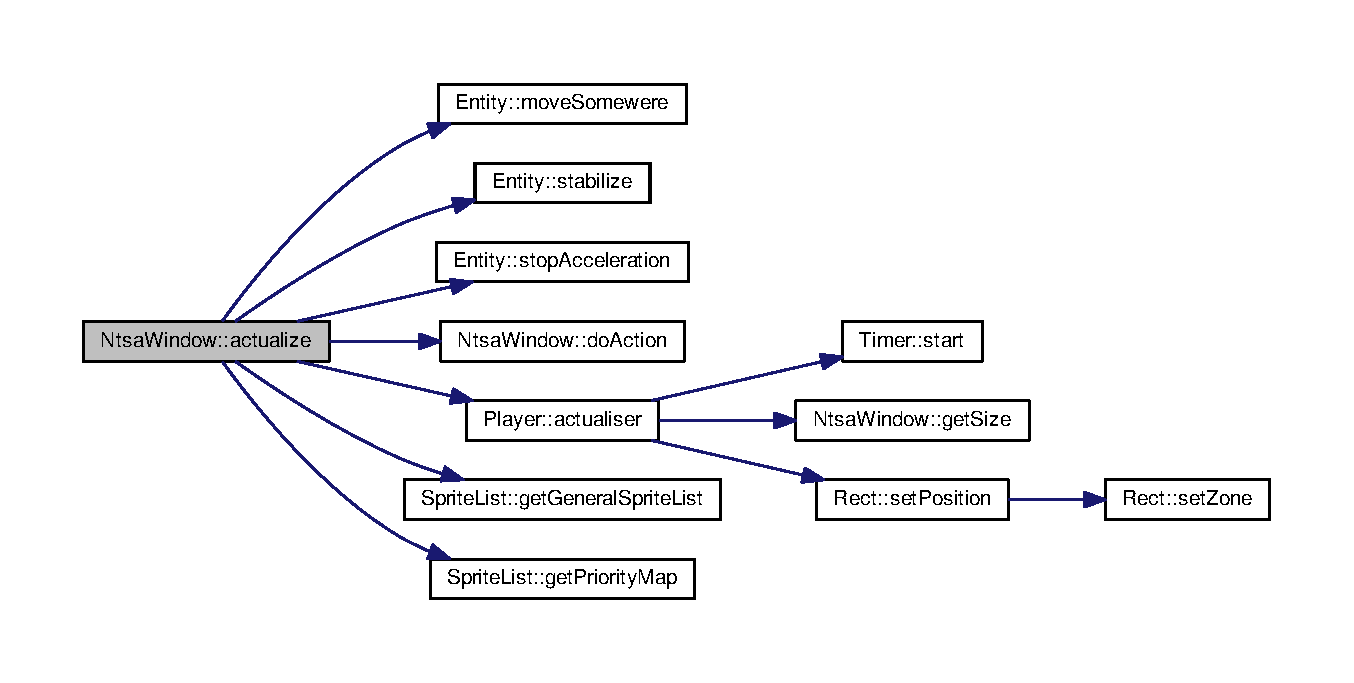
\includegraphics[width=350pt]{class_ntsa_window_aa8d0a7e8928dc1e90a4ca3616218f192_cgraph}
\end{center}
\end{figure}


\hypertarget{class_ntsa_window_ac2991e96dd1dc556961623824ddf682a}{\index{Ntsa\-Window@{Ntsa\-Window}!add\-Button@{add\-Button}}
\index{add\-Button@{add\-Button}!NtsaWindow@{Ntsa\-Window}}
\subsubsection[{add\-Button}]{\setlength{\rightskip}{0pt plus 5cm}void Ntsa\-Window\-::add\-Button (
\begin{DoxyParamCaption}
\item[{{\bf Button}}]{button}
\end{DoxyParamCaption}
)}}\label{class_ntsa_window_ac2991e96dd1dc556961623824ddf682a}


Definition at line 24 of file ntsa.\-cpp.



Here is the call graph for this function\-:\nopagebreak
\begin{figure}[H]
\begin{center}
\leavevmode
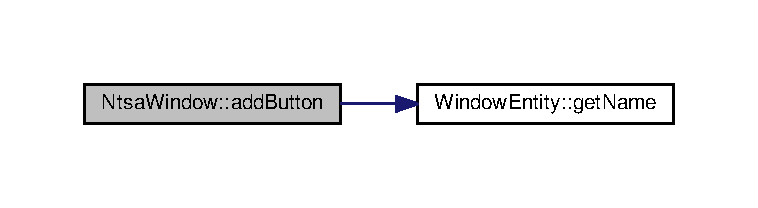
\includegraphics[width=350pt]{class_ntsa_window_ac2991e96dd1dc556961623824ddf682a_cgraph}
\end{center}
\end{figure}


\hypertarget{class_ntsa_window_a2ed76648e64d49378d9107eadd65feec}{\index{Ntsa\-Window@{Ntsa\-Window}!close@{close}}
\index{close@{close}!NtsaWindow@{Ntsa\-Window}}
\subsubsection[{close}]{\setlength{\rightskip}{0pt plus 5cm}void Ntsa\-Window\-::close (
\begin{DoxyParamCaption}
{}
\end{DoxyParamCaption}
)\hspace{0.3cm}{\ttfamily [inline]}}}\label{class_ntsa_window_a2ed76648e64d49378d9107eadd65feec}


Definition at line 30 of file ntsa.\-h.



Referenced by Main\-U\-I\-::\-Run().

\hypertarget{class_ntsa_window_ab0b4de4b43e6aa20fc96fbcc0805bad1}{\index{Ntsa\-Window@{Ntsa\-Window}!do\-Action@{do\-Action}}
\index{do\-Action@{do\-Action}!NtsaWindow@{Ntsa\-Window}}
\subsubsection[{do\-Action}]{\setlength{\rightskip}{0pt plus 5cm}void Ntsa\-Window\-::do\-Action (
\begin{DoxyParamCaption}
\item[{std\-::string}]{action}
\end{DoxyParamCaption}
)}}\label{class_ntsa_window_ab0b4de4b43e6aa20fc96fbcc0805bad1}


Definition at line 29 of file ntsa.\-cpp.



Referenced by actualize().

\hypertarget{class_ntsa_window_ab7f78dc06beb1fe676b21838f4f059e6}{\index{Ntsa\-Window@{Ntsa\-Window}!draw@{draw}}
\index{draw@{draw}!NtsaWindow@{Ntsa\-Window}}
\subsubsection[{draw}]{\setlength{\rightskip}{0pt plus 5cm}void Ntsa\-Window\-::draw (
\begin{DoxyParamCaption}
\item[{sf\-::\-Sprite $\ast$}]{sprite}
\end{DoxyParamCaption}
)\hspace{0.3cm}{\ttfamily [inline]}}}\label{class_ntsa_window_ab7f78dc06beb1fe676b21838f4f059e6}


Definition at line 31 of file ntsa.\-h.

\hypertarget{class_ntsa_window_ac38da02f04c79bc387308a89cd178538}{\index{Ntsa\-Window@{Ntsa\-Window}!get\-Relative\-Pos@{get\-Relative\-Pos}}
\index{get\-Relative\-Pos@{get\-Relative\-Pos}!NtsaWindow@{Ntsa\-Window}}
\subsubsection[{get\-Relative\-Pos}]{\setlength{\rightskip}{0pt plus 5cm}float Ntsa\-Window\-::get\-Relative\-Pos (
\begin{DoxyParamCaption}
\item[{{\bf Pos\-Names}}]{pos, }
\item[{int}]{factor}
\end{DoxyParamCaption}
)}}\label{class_ntsa_window_ac38da02f04c79bc387308a89cd178538}


Definition at line 35 of file ntsa.\-cpp.

\hypertarget{class_ntsa_window_a100372715e96061ae0a06c848e81383f}{\index{Ntsa\-Window@{Ntsa\-Window}!get\-Render\-Window@{get\-Render\-Window}}
\index{get\-Render\-Window@{get\-Render\-Window}!NtsaWindow@{Ntsa\-Window}}
\subsubsection[{get\-Render\-Window}]{\setlength{\rightskip}{0pt plus 5cm}sf\-::\-Render\-Window$\ast$ Ntsa\-Window\-::get\-Render\-Window (
\begin{DoxyParamCaption}
{}
\end{DoxyParamCaption}
)\hspace{0.3cm}{\ttfamily [inline]}}}\label{class_ntsa_window_a100372715e96061ae0a06c848e81383f}


Definition at line 25 of file ntsa.\-h.



Referenced by Main\-U\-I\-::\-Run().

\hypertarget{class_ntsa_window_a8504a8160e6c88968662c55ea4587f6c}{\index{Ntsa\-Window@{Ntsa\-Window}!get\-Size@{get\-Size}}
\index{get\-Size@{get\-Size}!NtsaWindow@{Ntsa\-Window}}
\subsubsection[{get\-Size}]{\setlength{\rightskip}{0pt plus 5cm}int Ntsa\-Window\-::get\-Size (
\begin{DoxyParamCaption}
\item[{{\bf Pos\-Names}}]{pos}
\end{DoxyParamCaption}
)}}\label{class_ntsa_window_a8504a8160e6c88968662c55ea4587f6c}


Definition at line 42 of file ntsa.\-cpp.



Referenced by Player\-::actualiser().

\hypertarget{class_ntsa_window_a04b0c18abd4bbe4a1785c633e17be351}{\index{Ntsa\-Window@{Ntsa\-Window}!get\-Width\-Height@{get\-Width\-Height}}
\index{get\-Width\-Height@{get\-Width\-Height}!NtsaWindow@{Ntsa\-Window}}
\subsubsection[{get\-Width\-Height}]{\setlength{\rightskip}{0pt plus 5cm}std\-::pair$<$int, int$>$ Ntsa\-Window\-::get\-Width\-Height (
\begin{DoxyParamCaption}
{}
\end{DoxyParamCaption}
)}}\label{class_ntsa_window_a04b0c18abd4bbe4a1785c633e17be351}
\hypertarget{class_ntsa_window_ad6b3a6571aeb24840953695a5ada4f42}{\index{Ntsa\-Window@{Ntsa\-Window}!is\-Open@{is\-Open}}
\index{is\-Open@{is\-Open}!NtsaWindow@{Ntsa\-Window}}
\subsubsection[{is\-Open}]{\setlength{\rightskip}{0pt plus 5cm}bool Ntsa\-Window\-::is\-Open (
\begin{DoxyParamCaption}
{}
\end{DoxyParamCaption}
)\hspace{0.3cm}{\ttfamily [inline]}}}\label{class_ntsa_window_ad6b3a6571aeb24840953695a5ada4f42}


Definition at line 32 of file ntsa.\-h.



Referenced by Main\-U\-I\-::\-Run().

\hypertarget{class_ntsa_window_a37708cfd4792e347f33c03e977475d9e}{\index{Ntsa\-Window@{Ntsa\-Window}!set\-Player@{set\-Player}}
\index{set\-Player@{set\-Player}!NtsaWindow@{Ntsa\-Window}}
\subsubsection[{set\-Player}]{\setlength{\rightskip}{0pt plus 5cm}void Ntsa\-Window\-::set\-Player (
\begin{DoxyParamCaption}
\item[{{\bf Player} $\ast$}]{player}
\end{DoxyParamCaption}
)}}\label{class_ntsa_window_a37708cfd4792e347f33c03e977475d9e}


Definition at line 19 of file ntsa.\-cpp.



\subsection{Field Documentation}
\hypertarget{class_ntsa_window_a05f52b64bbc047c05567c22cfb58471a}{\index{Ntsa\-Window@{Ntsa\-Window}!m\-\_\-buttons@{m\-\_\-buttons}}
\index{m\-\_\-buttons@{m\-\_\-buttons}!NtsaWindow@{Ntsa\-Window}}
\subsubsection[{m\-\_\-buttons}]{\setlength{\rightskip}{0pt plus 5cm}std\-::map$<$std\-::string, {\bf Button}$>$ Ntsa\-Window\-::m\-\_\-buttons\hspace{0.3cm}{\ttfamily [private]}}}\label{class_ntsa_window_a05f52b64bbc047c05567c22cfb58471a}


Definition at line 38 of file ntsa.\-h.



Referenced by actualize(), and add\-Button().

\hypertarget{class_ntsa_window_adda73a57cfa24bae0632d2b5272d0ac8}{\index{Ntsa\-Window@{Ntsa\-Window}!m\-\_\-player@{m\-\_\-player}}
\index{m\-\_\-player@{m\-\_\-player}!NtsaWindow@{Ntsa\-Window}}
\subsubsection[{m\-\_\-player}]{\setlength{\rightskip}{0pt plus 5cm}{\bf Player} Ntsa\-Window\-::m\-\_\-player\hspace{0.3cm}{\ttfamily [private]}}}\label{class_ntsa_window_adda73a57cfa24bae0632d2b5272d0ac8}


Definition at line 37 of file ntsa.\-h.



Referenced by actualize(), and set\-Player().

\hypertarget{class_ntsa_window_a6dec64dcc128fe25647d172cc28d7294}{\index{Ntsa\-Window@{Ntsa\-Window}!m\-\_\-window@{m\-\_\-window}}
\index{m\-\_\-window@{m\-\_\-window}!NtsaWindow@{Ntsa\-Window}}
\subsubsection[{m\-\_\-window}]{\setlength{\rightskip}{0pt plus 5cm}sf\-::\-Render\-Window$\ast$ Ntsa\-Window\-::m\-\_\-window\hspace{0.3cm}{\ttfamily [private]}}}\label{class_ntsa_window_a6dec64dcc128fe25647d172cc28d7294}


Definition at line 32 of file ntsa.\-h.



Referenced by actualize(), close(), do\-Action(), draw(), get\-Relative\-Pos(), get\-Render\-Window(), get\-Size(), and Ntsa\-Window().



The documentation for this class was generated from the following files\-:\begin{DoxyCompactItemize}
\item 
src/\-Graphics/\hyperlink{ntsa_8h}{ntsa.\-h}\item 
src/\-Graphics/\hyperlink{ntsa_8cpp}{ntsa.\-cpp}\end{DoxyCompactItemize}

\hypertarget{class_player}{\section{Player Class Reference}
\label{class_player}\index{Player@{Player}}
}


{\ttfamily \#include $<$entity.\-h$>$}



Inheritance diagram for Player\-:\nopagebreak
\begin{figure}[H]
\begin{center}
\leavevmode
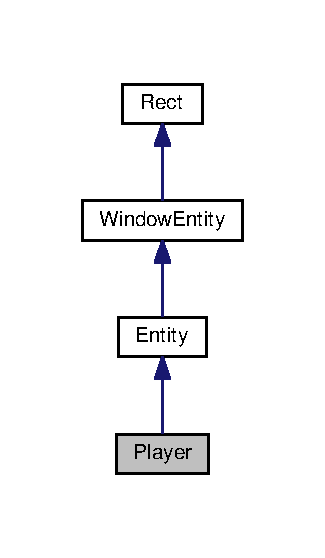
\includegraphics[width=156pt]{class_player__inherit__graph}
\end{center}
\end{figure}


Collaboration diagram for Player\-:\nopagebreak
\begin{figure}[H]
\begin{center}
\leavevmode
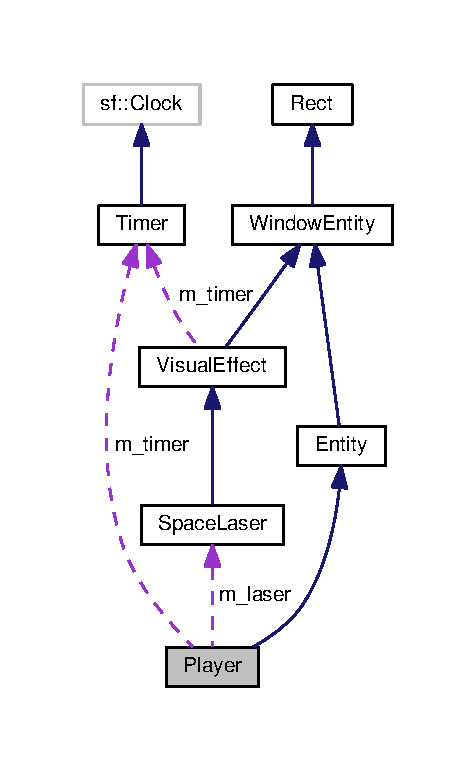
\includegraphics[width=228pt]{class_player__coll__graph}
\end{center}
\end{figure}
\subsection*{Public Member Functions}
\begin{DoxyCompactItemize}
\item 
\hyperlink{class_player_affe0cc3cb714f6deb4e62f0c0d3f1fd8}{Player} ()
\item 
\hyperlink{class_player_a6ac29a86604739284bdc303e219c3d32}{Player} (std\-::string name, unsigned int priority, std\-::string texture\-I\-D=\char`\"{}\char`\"{})
\item 
\hyperlink{class_player_a660212a54bd654ac1762467e00a2da31}{Player} (std\-::string name, unsigned int priority, unsigned int width, int position\-Y, std\-::string texture\-I\-D=\char`\"{}\char`\"{})
\item 
void \hyperlink{class_player_a4297433163d2c6b6a82b5d71c5362466}{actualiser} (\hyperlink{class_ntsa_window}{Ntsa\-Window} $\ast$window)
\item 
void \hyperlink{class_player_a5dc98bda088b0e253956ef22eba154f0}{fire} ()
\end{DoxyCompactItemize}
\subsection*{Private Attributes}
\begin{DoxyCompactItemize}
\item 
\hyperlink{class_timer}{Timer} \hyperlink{class_player_a384fd73bf7ac28a21e99e3512629db12}{m\-\_\-timer}
\item 
sf\-::\-Thread $\ast$ \hyperlink{class_player_aa80095e1a7cf10c0e6bd5d7a3e0f4c69}{m\-\_\-laser\-Thread} =nullptr
\item 
\hyperlink{class_space_laser}{Space\-Laser} \hyperlink{class_player_aff6ece5ac638c90cf670289c0d06def1}{m\-\_\-laser}
\item 
unsigned int \hyperlink{class_player_ad0e4c098b4e9ccd4356eeb630f6f9406}{m\-\_\-energy} =10000
\item 
float \hyperlink{class_player_af560153834486702db6a8a5b68ed4130}{m\-\_\-acceleration} =1.\-2
\item 
float \hyperlink{class_player_a9b6afe374aee047b49aa4c771b4495fc}{m\-\_\-step\-Multiplicator} =1.\-2
\begin{DoxyCompactList}\small\item\em L'accélération de base. \end{DoxyCompactList}\end{DoxyCompactItemize}
\subsection*{Additional Inherited Members}


\subsection{Detailed Description}


Definition at line 42 of file entity.\-h.



\subsection{Constructor \& Destructor Documentation}
\hypertarget{class_player_affe0cc3cb714f6deb4e62f0c0d3f1fd8}{\index{Player@{Player}!Player@{Player}}
\index{Player@{Player}!Player@{Player}}
\subsubsection[{Player}]{\setlength{\rightskip}{0pt plus 5cm}Player\-::\-Player (
\begin{DoxyParamCaption}
{}
\end{DoxyParamCaption}
)}}\label{class_player_affe0cc3cb714f6deb4e62f0c0d3f1fd8}


Definition at line 42 of file entity.\-cpp.

\hypertarget{class_player_a6ac29a86604739284bdc303e219c3d32}{\index{Player@{Player}!Player@{Player}}
\index{Player@{Player}!Player@{Player}}
\subsubsection[{Player}]{\setlength{\rightskip}{0pt plus 5cm}Player\-::\-Player (
\begin{DoxyParamCaption}
\item[{std\-::string}]{name, }
\item[{unsigned int}]{priority, }
\item[{std\-::string}]{texture\-I\-D = {\ttfamily \char`\"{}\char`\"{}}}
\end{DoxyParamCaption}
)}}\label{class_player_a6ac29a86604739284bdc303e219c3d32}


Definition at line 49 of file entity.\-cpp.

\hypertarget{class_player_a660212a54bd654ac1762467e00a2da31}{\index{Player@{Player}!Player@{Player}}
\index{Player@{Player}!Player@{Player}}
\subsubsection[{Player}]{\setlength{\rightskip}{0pt plus 5cm}Player\-::\-Player (
\begin{DoxyParamCaption}
\item[{std\-::string}]{name, }
\item[{unsigned int}]{priority, }
\item[{unsigned int}]{width, }
\item[{int}]{position\-Y, }
\item[{std\-::string}]{texture\-I\-D = {\ttfamily \char`\"{}\char`\"{}}}
\end{DoxyParamCaption}
)}}\label{class_player_a660212a54bd654ac1762467e00a2da31}


Definition at line 57 of file entity.\-cpp.



Here is the call graph for this function\-:\nopagebreak
\begin{figure}[H]
\begin{center}
\leavevmode
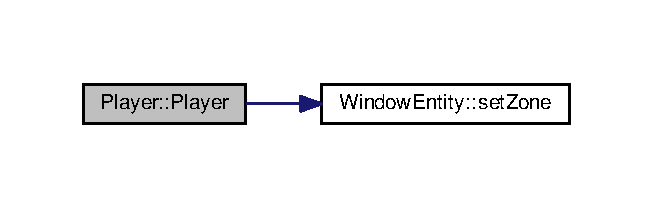
\includegraphics[width=314pt]{class_player_a660212a54bd654ac1762467e00a2da31_cgraph}
\end{center}
\end{figure}




\subsection{Member Function Documentation}
\hypertarget{class_player_a4297433163d2c6b6a82b5d71c5362466}{\index{Player@{Player}!actualiser@{actualiser}}
\index{actualiser@{actualiser}!Player@{Player}}
\subsubsection[{actualiser}]{\setlength{\rightskip}{0pt plus 5cm}void Player\-::actualiser (
\begin{DoxyParamCaption}
\item[{{\bf Ntsa\-Window} $\ast$}]{window}
\end{DoxyParamCaption}
)}}\label{class_player_a4297433163d2c6b6a82b5d71c5362466}


Definition at line 65 of file entity.\-cpp.



Referenced by Ntsa\-Window\-::actualize().



Here is the call graph for this function\-:\nopagebreak
\begin{figure}[H]
\begin{center}
\leavevmode
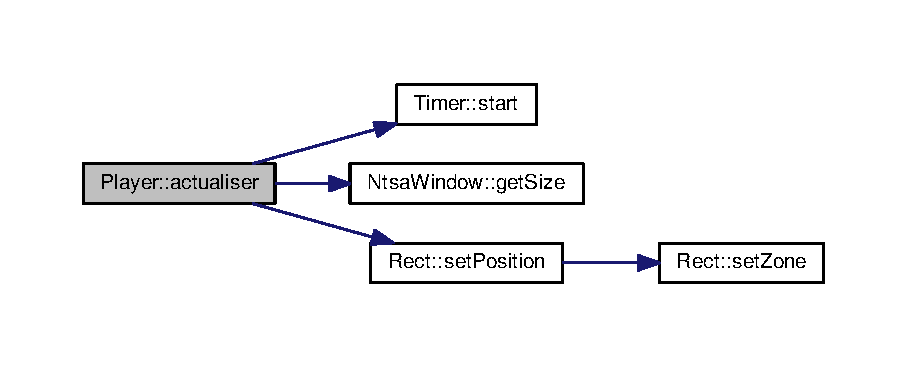
\includegraphics[width=350pt]{class_player_a4297433163d2c6b6a82b5d71c5362466_cgraph}
\end{center}
\end{figure}


\hypertarget{class_player_a5dc98bda088b0e253956ef22eba154f0}{\index{Player@{Player}!fire@{fire}}
\index{fire@{fire}!Player@{Player}}
\subsubsection[{fire}]{\setlength{\rightskip}{0pt plus 5cm}void Player\-::fire (
\begin{DoxyParamCaption}
{}
\end{DoxyParamCaption}
)}}\label{class_player_a5dc98bda088b0e253956ef22eba154f0}


Definition at line 107 of file entity.\-cpp.



\subsection{Field Documentation}
\hypertarget{class_player_af560153834486702db6a8a5b68ed4130}{\index{Player@{Player}!m\-\_\-acceleration@{m\-\_\-acceleration}}
\index{m\-\_\-acceleration@{m\-\_\-acceleration}!Player@{Player}}
\subsubsection[{m\-\_\-acceleration}]{\setlength{\rightskip}{0pt plus 5cm}float Player\-::m\-\_\-acceleration =1.\-2\hspace{0.3cm}{\ttfamily [private]}}}\label{class_player_af560153834486702db6a8a5b68ed4130}


Definition at line 58 of file entity.\-h.



Referenced by actualiser().

\hypertarget{class_player_ad0e4c098b4e9ccd4356eeb630f6f9406}{\index{Player@{Player}!m\-\_\-energy@{m\-\_\-energy}}
\index{m\-\_\-energy@{m\-\_\-energy}!Player@{Player}}
\subsubsection[{m\-\_\-energy}]{\setlength{\rightskip}{0pt plus 5cm}unsigned int Player\-::m\-\_\-energy =10000\hspace{0.3cm}{\ttfamily [private]}}}\label{class_player_ad0e4c098b4e9ccd4356eeb630f6f9406}


Definition at line 56 of file entity.\-h.

\hypertarget{class_player_aff6ece5ac638c90cf670289c0d06def1}{\index{Player@{Player}!m\-\_\-laser@{m\-\_\-laser}}
\index{m\-\_\-laser@{m\-\_\-laser}!Player@{Player}}
\subsubsection[{m\-\_\-laser}]{\setlength{\rightskip}{0pt plus 5cm}{\bf Space\-Laser} Player\-::m\-\_\-laser\hspace{0.3cm}{\ttfamily [private]}}}\label{class_player_aff6ece5ac638c90cf670289c0d06def1}


Definition at line 54 of file entity.\-h.



Referenced by Player().

\hypertarget{class_player_aa80095e1a7cf10c0e6bd5d7a3e0f4c69}{\index{Player@{Player}!m\-\_\-laser\-Thread@{m\-\_\-laser\-Thread}}
\index{m\-\_\-laser\-Thread@{m\-\_\-laser\-Thread}!Player@{Player}}
\subsubsection[{m\-\_\-laser\-Thread}]{\setlength{\rightskip}{0pt plus 5cm}sf\-::\-Thread$\ast$ Player\-::m\-\_\-laser\-Thread =nullptr\hspace{0.3cm}{\ttfamily [private]}}}\label{class_player_aa80095e1a7cf10c0e6bd5d7a3e0f4c69}


Definition at line 53 of file entity.\-h.

\hypertarget{class_player_a9b6afe374aee047b49aa4c771b4495fc}{\index{Player@{Player}!m\-\_\-step\-Multiplicator@{m\-\_\-step\-Multiplicator}}
\index{m\-\_\-step\-Multiplicator@{m\-\_\-step\-Multiplicator}!Player@{Player}}
\subsubsection[{m\-\_\-step\-Multiplicator}]{\setlength{\rightskip}{0pt plus 5cm}float Player\-::m\-\_\-step\-Multiplicator =1.\-2\hspace{0.3cm}{\ttfamily [private]}}}\label{class_player_a9b6afe374aee047b49aa4c771b4495fc}


L'accélération de base. 



Definition at line 59 of file entity.\-h.



Referenced by actualiser().

\hypertarget{class_player_a384fd73bf7ac28a21e99e3512629db12}{\index{Player@{Player}!m\-\_\-timer@{m\-\_\-timer}}
\index{m\-\_\-timer@{m\-\_\-timer}!Player@{Player}}
\subsubsection[{m\-\_\-timer}]{\setlength{\rightskip}{0pt plus 5cm}{\bf Timer} Player\-::m\-\_\-timer\hspace{0.3cm}{\ttfamily [private]}}}\label{class_player_a384fd73bf7ac28a21e99e3512629db12}


Definition at line 52 of file entity.\-h.



Referenced by actualiser(), and Player().



The documentation for this class was generated from the following files\-:\begin{DoxyCompactItemize}
\item 
src/\-Graphics/\hyperlink{entity_8h}{entity.\-h}\item 
src/\-Graphics/\hyperlink{entity_8cpp}{entity.\-cpp}\end{DoxyCompactItemize}

\input{struct_unoise_1_1point2_dui}
\hypertarget{class_public_rect}{\section{Public\-Rect Class Reference}
\label{class_public_rect}\index{Public\-Rect@{Public\-Rect}}
}


{\ttfamily \#include $<$rect.\-h$>$}

\subsection*{Public Member Functions}
\begin{DoxyCompactItemize}
\item 
\hyperlink{class_public_rect_af1b2a63089d11f607be5d0d912a50058}{Public\-Rect} ()
\item 
\hyperlink{class_public_rect_a4d664fdbc671fc4e3f1784d94687ed41}{Public\-Rect} (float x\-\_\-, float y\-\_\-)
\item 
\hyperlink{class_public_rect_a18365da833d896524b9d68f720154df2}{Public\-Rect} (float x\-\_\-, float y\-\_\-, float width\-\_\-, float height\-\_\-)
\end{DoxyCompactItemize}
\subsection*{Data Fields}
\begin{DoxyCompactItemize}
\item 
float \hyperlink{class_public_rect_a9b85ada3510a3d217471cd93f699624b}{x} =0
\item 
float \hyperlink{class_public_rect_ab37db90962870ddf84b7f8fbd62ab2ad}{y} =0
\item 
float \hyperlink{class_public_rect_ad9e87b1af7b2c11f35afaea9bd267871}{width} =0
\item 
float \hyperlink{class_public_rect_a9c2aef279c900310d3d0c8a351b7332f}{height} =0
\end{DoxyCompactItemize}


\subsection{Detailed Description}
Info\-: This class is very similary to sf\-::\-Rect of the S\-F\-M\-L -\/ Simple and Fast Multimedia Library wrote by Laurent Gomilla (\href{mailto:laurent@sfml-dev.org}{\tt laurent@sfml-\/dev.\-org}) Have a small thought to him! 

Definition at line 10 of file rect.\-h.



\subsection{Constructor \& Destructor Documentation}
\hypertarget{class_public_rect_af1b2a63089d11f607be5d0d912a50058}{\index{Public\-Rect@{Public\-Rect}!Public\-Rect@{Public\-Rect}}
\index{Public\-Rect@{Public\-Rect}!PublicRect@{Public\-Rect}}
\subsubsection[{Public\-Rect}]{\setlength{\rightskip}{0pt plus 5cm}Public\-Rect\-::\-Public\-Rect (
\begin{DoxyParamCaption}
{}
\end{DoxyParamCaption}
)\hspace{0.3cm}{\ttfamily [inline]}}}\label{class_public_rect_af1b2a63089d11f607be5d0d912a50058}


Definition at line 13 of file rect.\-h.

\hypertarget{class_public_rect_a4d664fdbc671fc4e3f1784d94687ed41}{\index{Public\-Rect@{Public\-Rect}!Public\-Rect@{Public\-Rect}}
\index{Public\-Rect@{Public\-Rect}!PublicRect@{Public\-Rect}}
\subsubsection[{Public\-Rect}]{\setlength{\rightskip}{0pt plus 5cm}Public\-Rect\-::\-Public\-Rect (
\begin{DoxyParamCaption}
\item[{float}]{x\-\_\-, }
\item[{float}]{y\-\_\-}
\end{DoxyParamCaption}
)\hspace{0.3cm}{\ttfamily [inline]}}}\label{class_public_rect_a4d664fdbc671fc4e3f1784d94687ed41}


Definition at line 14 of file rect.\-h.

\hypertarget{class_public_rect_a18365da833d896524b9d68f720154df2}{\index{Public\-Rect@{Public\-Rect}!Public\-Rect@{Public\-Rect}}
\index{Public\-Rect@{Public\-Rect}!PublicRect@{Public\-Rect}}
\subsubsection[{Public\-Rect}]{\setlength{\rightskip}{0pt plus 5cm}Public\-Rect\-::\-Public\-Rect (
\begin{DoxyParamCaption}
\item[{float}]{x\-\_\-, }
\item[{float}]{y\-\_\-, }
\item[{float}]{width\-\_\-, }
\item[{float}]{height\-\_\-}
\end{DoxyParamCaption}
)\hspace{0.3cm}{\ttfamily [inline]}}}\label{class_public_rect_a18365da833d896524b9d68f720154df2}


Definition at line 15 of file rect.\-h.



\subsection{Field Documentation}
\hypertarget{class_public_rect_a9c2aef279c900310d3d0c8a351b7332f}{\index{Public\-Rect@{Public\-Rect}!height@{height}}
\index{height@{height}!PublicRect@{Public\-Rect}}
\subsubsection[{height}]{\setlength{\rightskip}{0pt plus 5cm}float Public\-Rect\-::height =0}}\label{class_public_rect_a9c2aef279c900310d3d0c8a351b7332f}


Definition at line 16 of file rect.\-h.



Referenced by operator==().

\hypertarget{class_public_rect_ad9e87b1af7b2c11f35afaea9bd267871}{\index{Public\-Rect@{Public\-Rect}!width@{width}}
\index{width@{width}!PublicRect@{Public\-Rect}}
\subsubsection[{width}]{\setlength{\rightskip}{0pt plus 5cm}float Public\-Rect\-::width =0}}\label{class_public_rect_ad9e87b1af7b2c11f35afaea9bd267871}


Definition at line 16 of file rect.\-h.



Referenced by operator==().

\hypertarget{class_public_rect_a9b85ada3510a3d217471cd93f699624b}{\index{Public\-Rect@{Public\-Rect}!x@{x}}
\index{x@{x}!PublicRect@{Public\-Rect}}
\subsubsection[{x}]{\setlength{\rightskip}{0pt plus 5cm}float Public\-Rect\-::x =0}}\label{class_public_rect_a9b85ada3510a3d217471cd93f699624b}


Definition at line 16 of file rect.\-h.



Referenced by operator==().

\hypertarget{class_public_rect_ab37db90962870ddf84b7f8fbd62ab2ad}{\index{Public\-Rect@{Public\-Rect}!y@{y}}
\index{y@{y}!PublicRect@{Public\-Rect}}
\subsubsection[{y}]{\setlength{\rightskip}{0pt plus 5cm}float Public\-Rect\-::y =0}}\label{class_public_rect_ab37db90962870ddf84b7f8fbd62ab2ad}


Definition at line 16 of file rect.\-h.



Referenced by operator==().



The documentation for this class was generated from the following file\-:\begin{DoxyCompactItemize}
\item 
src/\-General/\hyperlink{rect_8h}{rect.\-h}\end{DoxyCompactItemize}

\hypertarget{class_rect}{\section{Rect Class Reference}
\label{class_rect}\index{Rect@{Rect}}
}


{\ttfamily \#include $<$rect.\-h$>$}



Inheritance diagram for Rect\-:\nopagebreak
\begin{figure}[H]
\begin{center}
\leavevmode
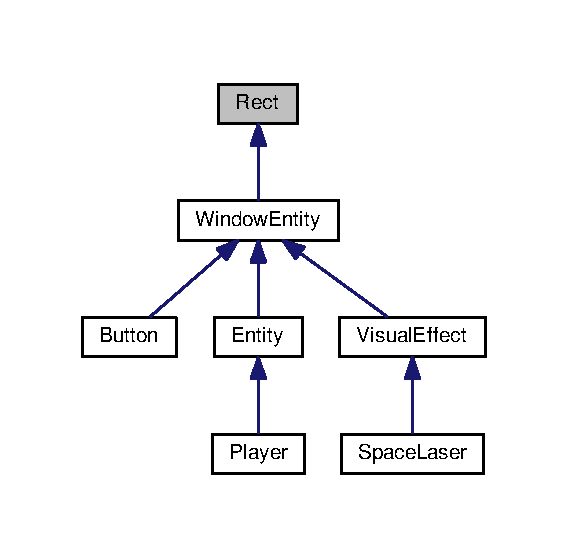
\includegraphics[width=273pt]{class_rect__inherit__graph}
\end{center}
\end{figure}
\subsection*{Public Member Functions}
\begin{DoxyCompactItemize}
\item 
\hyperlink{class_rect_a911e531b86de33734dd7de3456722115}{Rect} ()
\item 
\hyperlink{class_rect_ac039884b92bbdee68f7162036dfaefde}{Rect} (float rect\-Left, float rect\-Top, float rect\-Width, float rect\-Height)
\item 
\hyperlink{class_rect_aba3faa70ac657c788232b35719634196}{Rect} (const sf\-::\-Vector2f \&position, const sf\-::\-Vector2f \&size)
\item 
\hyperlink{class_rect_ac27e3c442eca764a0adbfbce7ecd679b}{Rect} (const \hyperlink{class_rect}{Rect} \&rectangle)
\item 
bool \hyperlink{class_rect_a4d0518ea473db46452c25044a95427ad}{contains} (float x, float y) const 
\item 
bool \hyperlink{class_rect_a98fe180ce28319ff319de5ab97fcc14c}{contains} (const sf\-::\-Vector2f \&point) const 
\item 
bool \hyperlink{class_rect_a77ef59c0903b538039bfeb3f4f03e198}{intersects} (const \hyperlink{class_rect}{Rect} \&rectangle) const 
\item 
bool \hyperlink{class_rect_a494a972edd829cb586333dfdd9c50b0a}{intersects} (const \hyperlink{class_rect}{Rect} \&rectangle, \hyperlink{class_rect}{Rect} \&intersection) const 
\item 
\hyperlink{class_public_rect}{Public\-Rect} \hyperlink{class_rect_a13d9cb2506258eda3787905452a9e7a3}{get\-Rect} ()
\item 
void \hyperlink{class_rect_a9c289437abe60bbb455c1b494a15eac3}{set\-Zone} (float new\-Pos\-X, float new\-Pos\-Y, float new\-Width=0, float new\-Height=0)
\item 
void \hyperlink{class_rect_ae4da133b058b25385e616496a0d35cc4}{set\-Width\-Height} (float new\-Width, float new\-Height)
\item 
void \hyperlink{class_rect_a7e6fca19d0ce00e318775d37631e2e0d}{set\-Position} (float new\-Pos\-X, float new\-Pos\-Y)
\end{DoxyCompactItemize}
\subsection*{Protected Attributes}
\begin{DoxyCompactItemize}
\item 
float \hyperlink{class_rect_aee32c031336a50f77c6cf882053e89f9}{m\-\_\-pos\-X}
\item 
float \hyperlink{class_rect_a10680ccabe0068eda6c9637aa6eeb2fd}{m\-\_\-pos\-Y}
\item 
float \hyperlink{class_rect_a2c4d58cb6e4d113e486913f62f47b558}{m\-\_\-width}
\item 
float \hyperlink{class_rect_a1cec6187b299195fd06daef55e6a96f1}{m\-\_\-height}
\end{DoxyCompactItemize}


\subsection{Detailed Description}


Definition at line 19 of file rect.\-h.



\subsection{Constructor \& Destructor Documentation}
\hypertarget{class_rect_a911e531b86de33734dd7de3456722115}{\index{Rect@{Rect}!Rect@{Rect}}
\index{Rect@{Rect}!Rect@{Rect}}
\subsubsection[{Rect}]{\setlength{\rightskip}{0pt plus 5cm}Rect\-::\-Rect (
\begin{DoxyParamCaption}
{}
\end{DoxyParamCaption}
)}}\label{class_rect_a911e531b86de33734dd7de3456722115}


Definition at line 3 of file rect.\-cpp.



Referenced by intersects().

\hypertarget{class_rect_ac039884b92bbdee68f7162036dfaefde}{\index{Rect@{Rect}!Rect@{Rect}}
\index{Rect@{Rect}!Rect@{Rect}}
\subsubsection[{Rect}]{\setlength{\rightskip}{0pt plus 5cm}Rect\-::\-Rect (
\begin{DoxyParamCaption}
\item[{float}]{rect\-Left, }
\item[{float}]{rect\-Top, }
\item[{float}]{rect\-Width, }
\item[{float}]{rect\-Height}
\end{DoxyParamCaption}
)}}\label{class_rect_ac039884b92bbdee68f7162036dfaefde}


Definition at line 13 of file rect.\-cpp.

\hypertarget{class_rect_aba3faa70ac657c788232b35719634196}{\index{Rect@{Rect}!Rect@{Rect}}
\index{Rect@{Rect}!Rect@{Rect}}
\subsubsection[{Rect}]{\setlength{\rightskip}{0pt plus 5cm}Rect\-::\-Rect (
\begin{DoxyParamCaption}
\item[{const sf\-::\-Vector2f \&}]{position, }
\item[{const sf\-::\-Vector2f \&}]{size}
\end{DoxyParamCaption}
)}}\label{class_rect_aba3faa70ac657c788232b35719634196}


Definition at line 23 of file rect.\-cpp.

\hypertarget{class_rect_ac27e3c442eca764a0adbfbce7ecd679b}{\index{Rect@{Rect}!Rect@{Rect}}
\index{Rect@{Rect}!Rect@{Rect}}
\subsubsection[{Rect}]{\setlength{\rightskip}{0pt plus 5cm}Rect\-::\-Rect (
\begin{DoxyParamCaption}
\item[{const {\bf Rect} \&}]{rectangle}
\end{DoxyParamCaption}
)\hspace{0.3cm}{\ttfamily [explicit]}}}\label{class_rect_ac27e3c442eca764a0adbfbce7ecd679b}


Definition at line 33 of file rect.\-cpp.



\subsection{Member Function Documentation}
\hypertarget{class_rect_a4d0518ea473db46452c25044a95427ad}{\index{Rect@{Rect}!contains@{contains}}
\index{contains@{contains}!Rect@{Rect}}
\subsubsection[{contains}]{\setlength{\rightskip}{0pt plus 5cm}bool Rect\-::contains (
\begin{DoxyParamCaption}
\item[{float}]{x, }
\item[{float}]{y}
\end{DoxyParamCaption}
) const}}\label{class_rect_a4d0518ea473db46452c25044a95427ad}


Definition at line 42 of file rect.\-cpp.



Referenced by contains().

\hypertarget{class_rect_a98fe180ce28319ff319de5ab97fcc14c}{\index{Rect@{Rect}!contains@{contains}}
\index{contains@{contains}!Rect@{Rect}}
\subsubsection[{contains}]{\setlength{\rightskip}{0pt plus 5cm}bool Rect\-::contains (
\begin{DoxyParamCaption}
\item[{const sf\-::\-Vector2f \&}]{point}
\end{DoxyParamCaption}
) const}}\label{class_rect_a98fe180ce28319ff319de5ab97fcc14c}


Definition at line 56 of file rect.\-cpp.



Here is the call graph for this function\-:\nopagebreak
\begin{figure}[H]
\begin{center}
\leavevmode
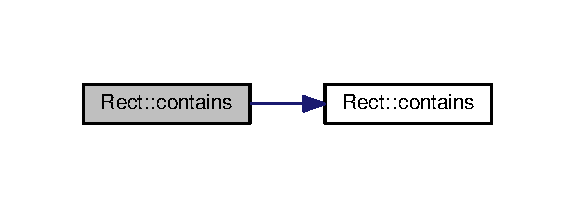
\includegraphics[width=276pt]{class_rect_a98fe180ce28319ff319de5ab97fcc14c_cgraph}
\end{center}
\end{figure}


\hypertarget{class_rect_a13d9cb2506258eda3787905452a9e7a3}{\index{Rect@{Rect}!get\-Rect@{get\-Rect}}
\index{get\-Rect@{get\-Rect}!Rect@{Rect}}
\subsubsection[{get\-Rect}]{\setlength{\rightskip}{0pt plus 5cm}{\bf Public\-Rect} Rect\-::get\-Rect (
\begin{DoxyParamCaption}
{}
\end{DoxyParamCaption}
)}}\label{class_rect_a13d9cb2506258eda3787905452a9e7a3}


Definition at line 68 of file rect.\-cpp.



Referenced by operator==().

\hypertarget{class_rect_a77ef59c0903b538039bfeb3f4f03e198}{\index{Rect@{Rect}!intersects@{intersects}}
\index{intersects@{intersects}!Rect@{Rect}}
\subsubsection[{intersects}]{\setlength{\rightskip}{0pt plus 5cm}bool Rect\-::intersects (
\begin{DoxyParamCaption}
\item[{const {\bf Rect} \&}]{rectangle}
\end{DoxyParamCaption}
) const}}\label{class_rect_a77ef59c0903b538039bfeb3f4f03e198}


Definition at line 62 of file rect.\-cpp.

\hypertarget{class_rect_a494a972edd829cb586333dfdd9c50b0a}{\index{Rect@{Rect}!intersects@{intersects}}
\index{intersects@{intersects}!Rect@{Rect}}
\subsubsection[{intersects}]{\setlength{\rightskip}{0pt plus 5cm}bool Rect\-::intersects (
\begin{DoxyParamCaption}
\item[{const {\bf Rect} \&}]{rectangle, }
\item[{{\bf Rect} \&}]{intersection}
\end{DoxyParamCaption}
) const}}\label{class_rect_a494a972edd829cb586333dfdd9c50b0a}


Definition at line 73 of file rect.\-cpp.



Here is the call graph for this function\-:\nopagebreak
\begin{figure}[H]
\begin{center}
\leavevmode
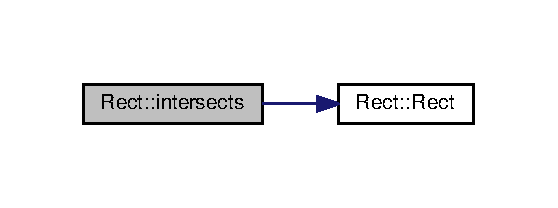
\includegraphics[width=268pt]{class_rect_a494a972edd829cb586333dfdd9c50b0a_cgraph}
\end{center}
\end{figure}


\hypertarget{class_rect_a7e6fca19d0ce00e318775d37631e2e0d}{\index{Rect@{Rect}!set\-Position@{set\-Position}}
\index{set\-Position@{set\-Position}!Rect@{Rect}}
\subsubsection[{set\-Position}]{\setlength{\rightskip}{0pt plus 5cm}void Rect\-::set\-Position (
\begin{DoxyParamCaption}
\item[{float}]{new\-Pos\-X, }
\item[{float}]{new\-Pos\-Y}
\end{DoxyParamCaption}
)}}\label{class_rect_a7e6fca19d0ce00e318775d37631e2e0d}


Definition at line 119 of file rect.\-cpp.



Referenced by Player\-::actualiser(), and Visual\-Effect\-::operator()().



Here is the call graph for this function\-:\nopagebreak
\begin{figure}[H]
\begin{center}
\leavevmode
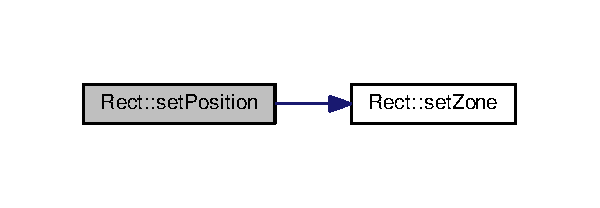
\includegraphics[width=288pt]{class_rect_a7e6fca19d0ce00e318775d37631e2e0d_cgraph}
\end{center}
\end{figure}


\hypertarget{class_rect_ae4da133b058b25385e616496a0d35cc4}{\index{Rect@{Rect}!set\-Width\-Height@{set\-Width\-Height}}
\index{set\-Width\-Height@{set\-Width\-Height}!Rect@{Rect}}
\subsubsection[{set\-Width\-Height}]{\setlength{\rightskip}{0pt plus 5cm}void Rect\-::set\-Width\-Height (
\begin{DoxyParamCaption}
\item[{float}]{new\-Width, }
\item[{float}]{new\-Height}
\end{DoxyParamCaption}
)}}\label{class_rect_ae4da133b058b25385e616496a0d35cc4}


Definition at line 124 of file rect.\-cpp.



Here is the call graph for this function\-:\nopagebreak
\begin{figure}[H]
\begin{center}
\leavevmode
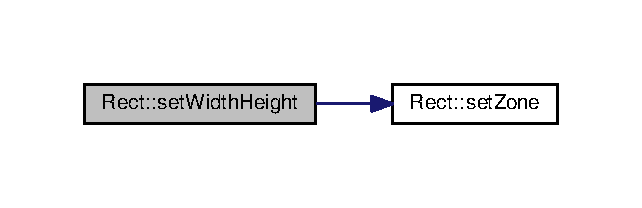
\includegraphics[width=308pt]{class_rect_ae4da133b058b25385e616496a0d35cc4_cgraph}
\end{center}
\end{figure}


\hypertarget{class_rect_a9c289437abe60bbb455c1b494a15eac3}{\index{Rect@{Rect}!set\-Zone@{set\-Zone}}
\index{set\-Zone@{set\-Zone}!Rect@{Rect}}
\subsubsection[{set\-Zone}]{\setlength{\rightskip}{0pt plus 5cm}void Rect\-::set\-Zone (
\begin{DoxyParamCaption}
\item[{float}]{new\-Pos\-X, }
\item[{float}]{new\-Pos\-Y, }
\item[{float}]{new\-Width = {\ttfamily 0}, }
\item[{float}]{new\-Height = {\ttfamily 0}}
\end{DoxyParamCaption}
)}}\label{class_rect_a9c289437abe60bbb455c1b494a15eac3}
\begin{DoxyNote}{Note}
Check 1 
\end{DoxyNote}


Definition at line 109 of file rect.\-cpp.



Referenced by set\-Position(), and set\-Width\-Height().



\subsection{Field Documentation}
\hypertarget{class_rect_a1cec6187b299195fd06daef55e6a96f1}{\index{Rect@{Rect}!m\-\_\-height@{m\-\_\-height}}
\index{m\-\_\-height@{m\-\_\-height}!Rect@{Rect}}
\subsubsection[{m\-\_\-height}]{\setlength{\rightskip}{0pt plus 5cm}float Rect\-::m\-\_\-height\hspace{0.3cm}{\ttfamily [protected]}}}\label{class_rect_a1cec6187b299195fd06daef55e6a96f1}


Definition at line 51 of file rect.\-h.



Referenced by Player\-::actualiser(), Window\-Entity\-::actuate\-Sprite(), contains(), get\-Rect(), intersects(), Button\-::is\-Pressed(), Player\-::\-Player(), Window\-Entity\-::set\-Zone(), set\-Zone(), and Visual\-Effect\-::\-Visual\-Effect().

\hypertarget{class_rect_aee32c031336a50f77c6cf882053e89f9}{\index{Rect@{Rect}!m\-\_\-pos\-X@{m\-\_\-pos\-X}}
\index{m\-\_\-pos\-X@{m\-\_\-pos\-X}!Rect@{Rect}}
\subsubsection[{m\-\_\-pos\-X}]{\setlength{\rightskip}{0pt plus 5cm}float Rect\-::m\-\_\-pos\-X\hspace{0.3cm}{\ttfamily [protected]}}}\label{class_rect_aee32c031336a50f77c6cf882053e89f9}


Definition at line 48 of file rect.\-h.



Referenced by Player\-::actualiser(), Window\-Entity\-::actuate\-Sprite(), contains(), get\-Rect(), intersects(), Button\-::is\-Pressed(), Visual\-Effect\-::operator()(), Player\-::\-Player(), set\-Width\-Height(), Window\-Entity\-::set\-Zone(), set\-Zone(), and Visual\-Effect\-::\-Visual\-Effect().

\hypertarget{class_rect_a10680ccabe0068eda6c9637aa6eeb2fd}{\index{Rect@{Rect}!m\-\_\-pos\-Y@{m\-\_\-pos\-Y}}
\index{m\-\_\-pos\-Y@{m\-\_\-pos\-Y}!Rect@{Rect}}
\subsubsection[{m\-\_\-pos\-Y}]{\setlength{\rightskip}{0pt plus 5cm}float Rect\-::m\-\_\-pos\-Y\hspace{0.3cm}{\ttfamily [protected]}}}\label{class_rect_a10680ccabe0068eda6c9637aa6eeb2fd}


Definition at line 49 of file rect.\-h.



Referenced by Player\-::actualiser(), Window\-Entity\-::actuate\-Sprite(), contains(), get\-Rect(), intersects(), Button\-::is\-Pressed(), Visual\-Effect\-::operator()(), Player\-::\-Player(), set\-Width\-Height(), Window\-Entity\-::set\-Zone(), set\-Zone(), and Visual\-Effect\-::\-Visual\-Effect().

\hypertarget{class_rect_a2c4d58cb6e4d113e486913f62f47b558}{\index{Rect@{Rect}!m\-\_\-width@{m\-\_\-width}}
\index{m\-\_\-width@{m\-\_\-width}!Rect@{Rect}}
\subsubsection[{m\-\_\-width}]{\setlength{\rightskip}{0pt plus 5cm}float Rect\-::m\-\_\-width\hspace{0.3cm}{\ttfamily [protected]}}}\label{class_rect_a2c4d58cb6e4d113e486913f62f47b558}


Definition at line 50 of file rect.\-h.



Referenced by Window\-Entity\-::actuate\-Sprite(), contains(), get\-Rect(), intersects(), Button\-::is\-Pressed(), Player\-::\-Player(), Window\-Entity\-::set\-Zone(), set\-Zone(), and Visual\-Effect\-::\-Visual\-Effect().



The documentation for this class was generated from the following files\-:\begin{DoxyCompactItemize}
\item 
src/\-General/\hyperlink{rect_8h}{rect.\-h}\item 
src/\-General/\hyperlink{rect_8cpp}{rect.\-cpp}\end{DoxyCompactItemize}

\hypertarget{class_space_laser}{\section{Space\-Laser Class Reference}
\label{class_space_laser}\index{Space\-Laser@{Space\-Laser}}
}


Cette classe ressemble en tout points à \hyperlink{class_visual_effect}{Visual\-Effect} mis à part un construxteur légèrement différent.  




{\ttfamily \#include $<$entity.\-h$>$}



Inheritance diagram for Space\-Laser\-:\nopagebreak
\begin{figure}[H]
\begin{center}
\leavevmode
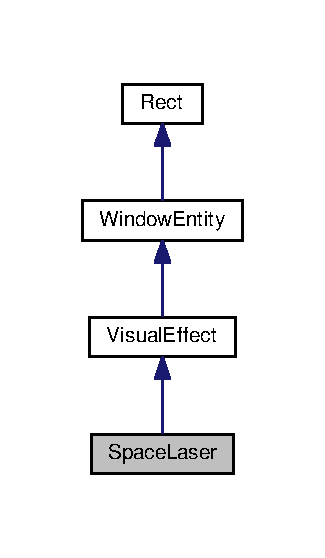
\includegraphics[width=156pt]{class_space_laser__inherit__graph}
\end{center}
\end{figure}


Collaboration diagram for Space\-Laser\-:\nopagebreak
\begin{figure}[H]
\begin{center}
\leavevmode
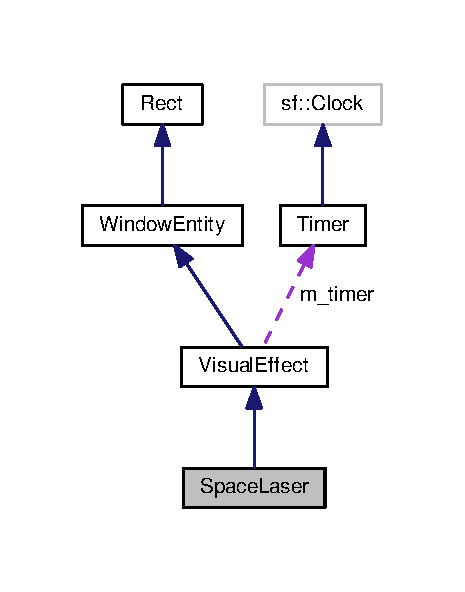
\includegraphics[width=223pt]{class_space_laser__coll__graph}
\end{center}
\end{figure}
\subsection*{Public Member Functions}
\begin{DoxyCompactItemize}
\item 
\hyperlink{class_space_laser_a5229629ac92a3948f3610a188c42899c}{Space\-Laser} ()
\item 
\hyperlink{class_space_laser_a6f66156fe9e311046555fa8ced7be4bb}{Space\-Laser} (float x, float y, float height, sf\-::\-Time cycle\-Duration, sf\-::\-Time duration=sf\-::seconds(0))
\end{DoxyCompactItemize}
\subsection*{Additional Inherited Members}


\subsection{Detailed Description}
Cette classe ressemble en tout points à \hyperlink{class_visual_effect}{Visual\-Effect} mis à part un construxteur légèrement différent. 

Definition at line 8 of file entity.\-h.



\subsection{Constructor \& Destructor Documentation}
\hypertarget{class_space_laser_a5229629ac92a3948f3610a188c42899c}{\index{Space\-Laser@{Space\-Laser}!Space\-Laser@{Space\-Laser}}
\index{Space\-Laser@{Space\-Laser}!SpaceLaser@{Space\-Laser}}
\subsubsection[{Space\-Laser}]{\setlength{\rightskip}{0pt plus 5cm}Space\-Laser\-::\-Space\-Laser (
\begin{DoxyParamCaption}
{}
\end{DoxyParamCaption}
)\hspace{0.3cm}{\ttfamily [inline]}}}\label{class_space_laser_a5229629ac92a3948f3610a188c42899c}


Definition at line 11 of file entity.\-h.

\hypertarget{class_space_laser_a6f66156fe9e311046555fa8ced7be4bb}{\index{Space\-Laser@{Space\-Laser}!Space\-Laser@{Space\-Laser}}
\index{Space\-Laser@{Space\-Laser}!SpaceLaser@{Space\-Laser}}
\subsubsection[{Space\-Laser}]{\setlength{\rightskip}{0pt plus 5cm}Space\-Laser\-::\-Space\-Laser (
\begin{DoxyParamCaption}
\item[{float}]{x, }
\item[{float}]{y, }
\item[{float}]{height, }
\item[{sf\-::\-Time}]{cycle\-Duration, }
\item[{sf\-::\-Time}]{duration = {\ttfamily sf\-:\-:seconds(0)}}
\end{DoxyParamCaption}
)}}\label{class_space_laser_a6f66156fe9e311046555fa8ced7be4bb}


Definition at line 122 of file entity.\-cpp.



The documentation for this class was generated from the following files\-:\begin{DoxyCompactItemize}
\item 
src/\-Graphics/\hyperlink{entity_8h}{entity.\-h}\item 
src/\-Graphics/\hyperlink{entity_8cpp}{entity.\-cpp}\end{DoxyCompactItemize}

\hypertarget{class_sprite_list}{\section{Sprite\-List Class Reference}
\label{class_sprite_list}\index{Sprite\-List@{Sprite\-List}}
}


{\ttfamily \#include $<$general.\-h$>$}

\subsection*{Public Member Functions}
\begin{DoxyCompactItemize}
\item 
\hyperlink{class_sprite_list_a73c339180c9a10829d376833ebf3f88a}{Sprite\-List} ()
\item 
sf\-::\-Sprite $\ast$ \hyperlink{class_sprite_list_a1f9cb9cef32d7b73e83539a8fc84c05d}{Add\-Sprite} (sf\-::\-Sprite sprite, std\-::string id, unsigned int priority)
\item 
void \hyperlink{class_sprite_list_acab29c36364d8b684e6d82d381a3a834}{Remove\-Sprite} (std\-::string id)
\item 
std\-::multimap$<$ unsigned int, \\*
sf\-::\-Sprite $\ast$ $>$ $\ast$ \hyperlink{class_sprite_list_a231c6090b04c2b0ba261f9ce5e3d1f1c}{get\-Priority\-Map} ()
\end{DoxyCompactItemize}
\subsection*{Static Public Member Functions}
\begin{DoxyCompactItemize}
\item 
static \hyperlink{class_sprite_list}{Sprite\-List} $\ast$ \hyperlink{class_sprite_list_a31aad8d098174638df4d85fae19d9176}{get\-General\-Sprite\-List} ()
\end{DoxyCompactItemize}
\subsection*{Private Attributes}
\begin{DoxyCompactItemize}
\item 
std\-::map$<$ std\-::string, \\*
sf\-::\-Sprite $\ast$ $>$ \hyperlink{class_sprite_list_aa0ca6f88f303676cb1592098cf4a38ea}{index\-Map}
\item 
std\-::multimap$<$ unsigned int, \\*
sf\-::\-Sprite $\ast$ $>$ \hyperlink{class_sprite_list_a79da3c65e989060ad28f5bb2690e757b}{priority\-Map}
\end{DoxyCompactItemize}


\subsection{Detailed Description}


Definition at line 26 of file general.\-h.



\subsection{Constructor \& Destructor Documentation}
\hypertarget{class_sprite_list_a73c339180c9a10829d376833ebf3f88a}{\index{Sprite\-List@{Sprite\-List}!Sprite\-List@{Sprite\-List}}
\index{Sprite\-List@{Sprite\-List}!SpriteList@{Sprite\-List}}
\subsubsection[{Sprite\-List}]{\setlength{\rightskip}{0pt plus 5cm}Sprite\-List\-::\-Sprite\-List (
\begin{DoxyParamCaption}
{}
\end{DoxyParamCaption}
)\hspace{0.3cm}{\ttfamily [inline]}}}\label{class_sprite_list_a73c339180c9a10829d376833ebf3f88a}


Definition at line 29 of file general.\-h.



\subsection{Member Function Documentation}
\hypertarget{class_sprite_list_a1f9cb9cef32d7b73e83539a8fc84c05d}{\index{Sprite\-List@{Sprite\-List}!Add\-Sprite@{Add\-Sprite}}
\index{Add\-Sprite@{Add\-Sprite}!SpriteList@{Sprite\-List}}
\subsubsection[{Add\-Sprite}]{\setlength{\rightskip}{0pt plus 5cm}sf\-::\-Sprite $\ast$ Sprite\-List\-::\-Add\-Sprite (
\begin{DoxyParamCaption}
\item[{sf\-::\-Sprite}]{sprite, }
\item[{std\-::string}]{id, }
\item[{unsigned int}]{priority}
\end{DoxyParamCaption}
)}}\label{class_sprite_list_a1f9cb9cef32d7b73e83539a8fc84c05d}
\begin{DoxyReturn}{Returns}
Le sprite reset 
\end{DoxyReturn}


Definition at line 21 of file general.\-cpp.



Referenced by Window\-Entity\-::actuate\-Sprite().

\hypertarget{class_sprite_list_a31aad8d098174638df4d85fae19d9176}{\index{Sprite\-List@{Sprite\-List}!get\-General\-Sprite\-List@{get\-General\-Sprite\-List}}
\index{get\-General\-Sprite\-List@{get\-General\-Sprite\-List}!SpriteList@{Sprite\-List}}
\subsubsection[{get\-General\-Sprite\-List}]{\setlength{\rightskip}{0pt plus 5cm}{\bf Sprite\-List} $\ast$ Sprite\-List\-::get\-General\-Sprite\-List (
\begin{DoxyParamCaption}
{}
\end{DoxyParamCaption}
)\hspace{0.3cm}{\ttfamily [static]}}}\label{class_sprite_list_a31aad8d098174638df4d85fae19d9176}


Definition at line 7 of file general.\-cpp.



Referenced by Ntsa\-Window\-::actualize(), and Window\-Entity\-::actuate\-Sprite().

\hypertarget{class_sprite_list_a231c6090b04c2b0ba261f9ce5e3d1f1c}{\index{Sprite\-List@{Sprite\-List}!get\-Priority\-Map@{get\-Priority\-Map}}
\index{get\-Priority\-Map@{get\-Priority\-Map}!SpriteList@{Sprite\-List}}
\subsubsection[{get\-Priority\-Map}]{\setlength{\rightskip}{0pt plus 5cm}std\-::multimap$<$unsigned int, sf\-::\-Sprite$\ast$$>$$\ast$ Sprite\-List\-::get\-Priority\-Map (
\begin{DoxyParamCaption}
{}
\end{DoxyParamCaption}
)\hspace{0.3cm}{\ttfamily [inline]}}}\label{class_sprite_list_a231c6090b04c2b0ba261f9ce5e3d1f1c}


Definition at line 34 of file general.\-h.



Referenced by Ntsa\-Window\-::actualize().

\hypertarget{class_sprite_list_acab29c36364d8b684e6d82d381a3a834}{\index{Sprite\-List@{Sprite\-List}!Remove\-Sprite@{Remove\-Sprite}}
\index{Remove\-Sprite@{Remove\-Sprite}!SpriteList@{Sprite\-List}}
\subsubsection[{Remove\-Sprite}]{\setlength{\rightskip}{0pt plus 5cm}void Sprite\-List\-::\-Remove\-Sprite (
\begin{DoxyParamCaption}
\item[{std\-::string}]{id}
\end{DoxyParamCaption}
)}}\label{class_sprite_list_acab29c36364d8b684e6d82d381a3a834}
\begin{DoxyNote}{Note}
check 1 
\end{DoxyNote}


Definition at line 49 of file general.\-cpp.



\subsection{Field Documentation}
\hypertarget{class_sprite_list_aa0ca6f88f303676cb1592098cf4a38ea}{\index{Sprite\-List@{Sprite\-List}!index\-Map@{index\-Map}}
\index{index\-Map@{index\-Map}!SpriteList@{Sprite\-List}}
\subsubsection[{index\-Map}]{\setlength{\rightskip}{0pt plus 5cm}std\-::map$<$std\-::string, sf\-::\-Sprite$\ast$$>$ Sprite\-List\-::index\-Map\hspace{0.3cm}{\ttfamily [private]}}}\label{class_sprite_list_aa0ca6f88f303676cb1592098cf4a38ea}


Definition at line 34 of file general.\-h.



Referenced by Add\-Sprite(), and Remove\-Sprite().

\hypertarget{class_sprite_list_a79da3c65e989060ad28f5bb2690e757b}{\index{Sprite\-List@{Sprite\-List}!priority\-Map@{priority\-Map}}
\index{priority\-Map@{priority\-Map}!SpriteList@{Sprite\-List}}
\subsubsection[{priority\-Map}]{\setlength{\rightskip}{0pt plus 5cm}std\-::multimap$<$unsigned int, sf\-::\-Sprite$\ast$$>$ Sprite\-List\-::priority\-Map\hspace{0.3cm}{\ttfamily [private]}}}\label{class_sprite_list_a79da3c65e989060ad28f5bb2690e757b}


Definition at line 38 of file general.\-h.



Referenced by Add\-Sprite(), and Remove\-Sprite().



The documentation for this class was generated from the following files\-:\begin{DoxyCompactItemize}
\item 
src/\-General/\hyperlink{general_8h}{general.\-h}\item 
src/\-General/\hyperlink{general_8cpp}{general.\-cpp}\end{DoxyCompactItemize}

\hypertarget{class_texture_list}{\section{Texture\-List Class Reference}
\label{class_texture_list}\index{Texture\-List@{Texture\-List}}
}


{\ttfamily \#include $<$general.\-h$>$}

\subsection*{Public Member Functions}
\begin{DoxyCompactItemize}
\item 
\hyperlink{class_texture_list_a750d37ace9aed214e8cbe1f940faf06f}{Texture\-List} ()
\item 
\hyperlink{class_texture_list_af10f38dd97933b3efd473b0bd2bafa77}{Texture\-List} (std\-::string file\-Path)
\item 
void \hyperlink{class_texture_list_a4c8c84b6df51995e568d7119d70f89a7}{load\-Textures} (std\-::string file\-Path)
\item 
void \hyperlink{class_texture_list_ade252d75b421d1b1a7ada32240e5c131}{show\-Errors} (std\-::string outfilen=\char`\"{}\char`\"{})
\item 
sf\-::\-Texture $\ast$ \hyperlink{class_texture_list_a27e768ab0f66150d4b45b5d4d0f08e4b}{get\-Texture} (std\-::string texture\-I\-D)
\end{DoxyCompactItemize}
\subsection*{Static Public Member Functions}
\begin{DoxyCompactItemize}
\item 
static \hyperlink{class_texture_list}{Texture\-List} $\ast$ \hyperlink{class_texture_list_ab97506e3c31990bf341103d1d4589829}{get\-General\-Texture\-List} ()
\end{DoxyCompactItemize}
\subsection*{Private Attributes}
\begin{DoxyCompactItemize}
\item 
std\-::string \hyperlink{class_texture_list_accfab4bb10cf490ab44f24a721bd9849}{m\-\_\-errors}
\item 
std\-::map$<$ std\-::string, \\*
sf\-::\-Texture $>$ \hyperlink{class_texture_list_a1e82ecc17a450b6afa112753bcaf139e}{m\-\_\-texture\-Map}
\end{DoxyCompactItemize}


\subsection{Detailed Description}


Definition at line 41 of file general.\-h.



\subsection{Constructor \& Destructor Documentation}
\hypertarget{class_texture_list_a750d37ace9aed214e8cbe1f940faf06f}{\index{Texture\-List@{Texture\-List}!Texture\-List@{Texture\-List}}
\index{Texture\-List@{Texture\-List}!TextureList@{Texture\-List}}
\subsubsection[{Texture\-List}]{\setlength{\rightskip}{0pt plus 5cm}Texture\-List\-::\-Texture\-List (
\begin{DoxyParamCaption}
{}
\end{DoxyParamCaption}
)\hspace{0.3cm}{\ttfamily [inline]}}}\label{class_texture_list_a750d37ace9aed214e8cbe1f940faf06f}


Definition at line 44 of file general.\-h.

\hypertarget{class_texture_list_af10f38dd97933b3efd473b0bd2bafa77}{\index{Texture\-List@{Texture\-List}!Texture\-List@{Texture\-List}}
\index{Texture\-List@{Texture\-List}!TextureList@{Texture\-List}}
\subsubsection[{Texture\-List}]{\setlength{\rightskip}{0pt plus 5cm}Texture\-List\-::\-Texture\-List (
\begin{DoxyParamCaption}
\item[{std\-::string}]{file\-Path}
\end{DoxyParamCaption}
)}}\label{class_texture_list_af10f38dd97933b3efd473b0bd2bafa77}
\begin{DoxyNote}{Note}
check 1 
\end{DoxyNote}


Definition at line 73 of file general.\-cpp.



Here is the call graph for this function\-:\nopagebreak
\begin{figure}[H]
\begin{center}
\leavevmode
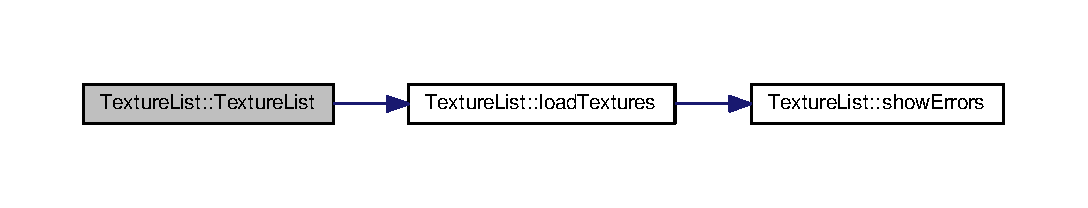
\includegraphics[width=350pt]{class_texture_list_af10f38dd97933b3efd473b0bd2bafa77_cgraph}
\end{center}
\end{figure}




\subsection{Member Function Documentation}
\hypertarget{class_texture_list_ab97506e3c31990bf341103d1d4589829}{\index{Texture\-List@{Texture\-List}!get\-General\-Texture\-List@{get\-General\-Texture\-List}}
\index{get\-General\-Texture\-List@{get\-General\-Texture\-List}!TextureList@{Texture\-List}}
\subsubsection[{get\-General\-Texture\-List}]{\setlength{\rightskip}{0pt plus 5cm}{\bf Texture\-List} $\ast$ Texture\-List\-::get\-General\-Texture\-List (
\begin{DoxyParamCaption}
{}
\end{DoxyParamCaption}
)\hspace{0.3cm}{\ttfamily [static]}}}\label{class_texture_list_ab97506e3c31990bf341103d1d4589829}


Definition at line 12 of file general.\-cpp.



Referenced by Window\-Entity\-::add\-Texture().

\hypertarget{class_texture_list_a27e768ab0f66150d4b45b5d4d0f08e4b}{\index{Texture\-List@{Texture\-List}!get\-Texture@{get\-Texture}}
\index{get\-Texture@{get\-Texture}!TextureList@{Texture\-List}}
\subsubsection[{get\-Texture}]{\setlength{\rightskip}{0pt plus 5cm}sf\-::\-Texture $\ast$ Texture\-List\-::get\-Texture (
\begin{DoxyParamCaption}
\item[{std\-::string}]{texture\-I\-D}
\end{DoxyParamCaption}
)}}\label{class_texture_list_a27e768ab0f66150d4b45b5d4d0f08e4b}


Definition at line 128 of file general.\-cpp.



Referenced by Window\-Entity\-::add\-Texture().

\hypertarget{class_texture_list_a4c8c84b6df51995e568d7119d70f89a7}{\index{Texture\-List@{Texture\-List}!load\-Textures@{load\-Textures}}
\index{load\-Textures@{load\-Textures}!TextureList@{Texture\-List}}
\subsubsection[{load\-Textures}]{\setlength{\rightskip}{0pt plus 5cm}void Texture\-List\-::load\-Textures (
\begin{DoxyParamCaption}
\item[{std\-::string}]{file\-Path}
\end{DoxyParamCaption}
)}}\label{class_texture_list_a4c8c84b6df51995e568d7119d70f89a7}
\begin{DoxyNote}{Note}
check 1 
\end{DoxyNote}


Definition at line 93 of file general.\-cpp.



Referenced by Texture\-List().



Here is the call graph for this function\-:\nopagebreak
\begin{figure}[H]
\begin{center}
\leavevmode
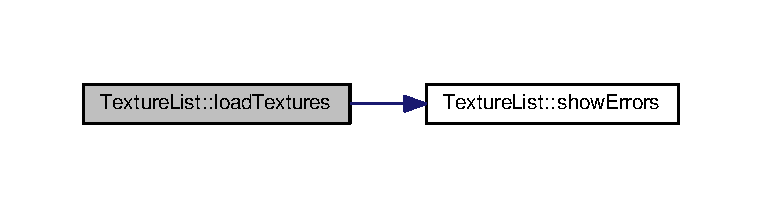
\includegraphics[width=350pt]{class_texture_list_a4c8c84b6df51995e568d7119d70f89a7_cgraph}
\end{center}
\end{figure}


\hypertarget{class_texture_list_ade252d75b421d1b1a7ada32240e5c131}{\index{Texture\-List@{Texture\-List}!show\-Errors@{show\-Errors}}
\index{show\-Errors@{show\-Errors}!TextureList@{Texture\-List}}
\subsubsection[{show\-Errors}]{\setlength{\rightskip}{0pt plus 5cm}void Texture\-List\-::show\-Errors (
\begin{DoxyParamCaption}
\item[{std\-::string}]{outfilen = {\ttfamily \char`\"{}\char`\"{}}}
\end{DoxyParamCaption}
)}}\label{class_texture_list_ade252d75b421d1b1a7ada32240e5c131}
\begin{DoxyNote}{Note}
check 1 
\end{DoxyNote}


Definition at line 78 of file general.\-cpp.



Referenced by load\-Textures().



\subsection{Field Documentation}
\hypertarget{class_texture_list_accfab4bb10cf490ab44f24a721bd9849}{\index{Texture\-List@{Texture\-List}!m\-\_\-errors@{m\-\_\-errors}}
\index{m\-\_\-errors@{m\-\_\-errors}!TextureList@{Texture\-List}}
\subsubsection[{m\-\_\-errors}]{\setlength{\rightskip}{0pt plus 5cm}std\-::string Texture\-List\-::m\-\_\-errors\hspace{0.3cm}{\ttfamily [private]}}}\label{class_texture_list_accfab4bb10cf490ab44f24a721bd9849}


Definition at line 53 of file general.\-h.



Referenced by load\-Textures(), and show\-Errors().

\hypertarget{class_texture_list_a1e82ecc17a450b6afa112753bcaf139e}{\index{Texture\-List@{Texture\-List}!m\-\_\-texture\-Map@{m\-\_\-texture\-Map}}
\index{m\-\_\-texture\-Map@{m\-\_\-texture\-Map}!TextureList@{Texture\-List}}
\subsubsection[{m\-\_\-texture\-Map}]{\setlength{\rightskip}{0pt plus 5cm}std\-::map$<$std\-::string, sf\-::\-Texture$>$ Texture\-List\-::m\-\_\-texture\-Map\hspace{0.3cm}{\ttfamily [private]}}}\label{class_texture_list_a1e82ecc17a450b6afa112753bcaf139e}


Definition at line 54 of file general.\-h.



Referenced by get\-Texture(), and load\-Textures().



The documentation for this class was generated from the following files\-:\begin{DoxyCompactItemize}
\item 
src/\-General/\hyperlink{general_8h}{general.\-h}\item 
src/\-General/\hyperlink{general_8cpp}{general.\-cpp}\end{DoxyCompactItemize}

\hypertarget{class_timer}{\section{Timer Class Reference}
\label{class_timer}\index{Timer@{Timer}}
}


{\ttfamily \#include $<$general.\-h$>$}



Inheritance diagram for Timer\-:\nopagebreak
\begin{figure}[H]
\begin{center}
\leavevmode
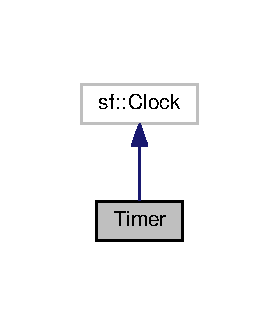
\includegraphics[width=134pt]{class_timer__inherit__graph}
\end{center}
\end{figure}


Collaboration diagram for Timer\-:\nopagebreak
\begin{figure}[H]
\begin{center}
\leavevmode
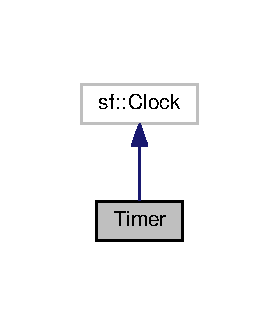
\includegraphics[width=134pt]{class_timer__coll__graph}
\end{center}
\end{figure}
\subsection*{Public Member Functions}
\begin{DoxyCompactItemize}
\item 
\hyperlink{class_timer_a5f16e8da27d2a5a5242dead46de05d97}{Timer} ()
\item 
void \hyperlink{class_timer_a3a8b5272198d029779dc9302a54305a8}{start} ()
\begin{DoxyCompactList}\small\item\em Restart le timer uniquement la première fois ou quand stop a été appelé juste avant. \end{DoxyCompactList}\item 
void \hyperlink{class_timer_a63f0eb44b27402196590a03781515dba}{stop} ()
\begin{DoxyCompactList}\small\item\em Permet un nouvel appel à start. \end{DoxyCompactList}\end{DoxyCompactItemize}
\subsection*{Private Attributes}
\begin{DoxyCompactItemize}
\item 
bool \hyperlink{class_timer_ab82f1b382db2231bf358bb6ec5dbe45d}{m\-\_\-started} =false
\end{DoxyCompactItemize}


\subsection{Detailed Description}


Definition at line 14 of file general.\-h.



\subsection{Constructor \& Destructor Documentation}
\hypertarget{class_timer_a5f16e8da27d2a5a5242dead46de05d97}{\index{Timer@{Timer}!Timer@{Timer}}
\index{Timer@{Timer}!Timer@{Timer}}
\subsubsection[{Timer}]{\setlength{\rightskip}{0pt plus 5cm}Timer\-::\-Timer (
\begin{DoxyParamCaption}
{}
\end{DoxyParamCaption}
)\hspace{0.3cm}{\ttfamily [inline]}}}\label{class_timer_a5f16e8da27d2a5a5242dead46de05d97}


Definition at line 17 of file general.\-h.



\subsection{Member Function Documentation}
\hypertarget{class_timer_a3a8b5272198d029779dc9302a54305a8}{\index{Timer@{Timer}!start@{start}}
\index{start@{start}!Timer@{Timer}}
\subsubsection[{start}]{\setlength{\rightskip}{0pt plus 5cm}void Timer\-::start (
\begin{DoxyParamCaption}
{}
\end{DoxyParamCaption}
)}}\label{class_timer_a3a8b5272198d029779dc9302a54305a8}


Restart le timer uniquement la première fois ou quand stop a été appelé juste avant. 



Definition at line 137 of file general.\-cpp.



Referenced by Player\-::actualiser().

\hypertarget{class_timer_a63f0eb44b27402196590a03781515dba}{\index{Timer@{Timer}!stop@{stop}}
\index{stop@{stop}!Timer@{Timer}}
\subsubsection[{stop}]{\setlength{\rightskip}{0pt plus 5cm}void Timer\-::stop (
\begin{DoxyParamCaption}
{}
\end{DoxyParamCaption}
)}}\label{class_timer_a63f0eb44b27402196590a03781515dba}


Permet un nouvel appel à start. 



Definition at line 146 of file general.\-cpp.



\subsection{Field Documentation}
\hypertarget{class_timer_ab82f1b382db2231bf358bb6ec5dbe45d}{\index{Timer@{Timer}!m\-\_\-started@{m\-\_\-started}}
\index{m\-\_\-started@{m\-\_\-started}!Timer@{Timer}}
\subsubsection[{m\-\_\-started}]{\setlength{\rightskip}{0pt plus 5cm}bool Timer\-::m\-\_\-started =false\hspace{0.3cm}{\ttfamily [private]}}}\label{class_timer_ab82f1b382db2231bf358bb6ec5dbe45d}


Definition at line 23 of file general.\-h.



Referenced by start(), and stop().



The documentation for this class was generated from the following files\-:\begin{DoxyCompactItemize}
\item 
src/\-General/\hyperlink{general_8h}{general.\-h}\item 
src/\-General/\hyperlink{general_8cpp}{general.\-cpp}\end{DoxyCompactItemize}

\hypertarget{class_visual_effect}{\section{Visual\-Effect Class Reference}
\label{class_visual_effect}\index{Visual\-Effect@{Visual\-Effect}}
}


Une classe gérant effet visuel temporaire.  




{\ttfamily \#include $<$Window\-Entity.\-h$>$}



Inheritance diagram for Visual\-Effect\-:\nopagebreak
\begin{figure}[H]
\begin{center}
\leavevmode
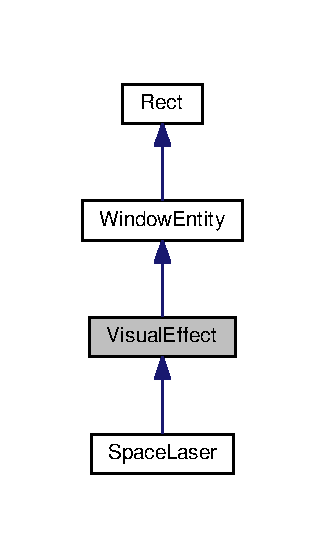
\includegraphics[width=156pt]{class_visual_effect__inherit__graph}
\end{center}
\end{figure}


Collaboration diagram for Visual\-Effect\-:\nopagebreak
\begin{figure}[H]
\begin{center}
\leavevmode
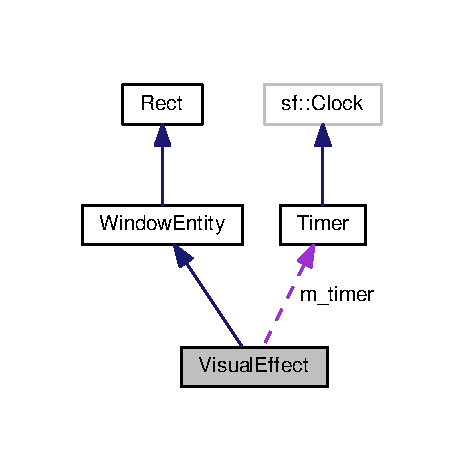
\includegraphics[width=223pt]{class_visual_effect__coll__graph}
\end{center}
\end{figure}
\subsection*{Public Types}
\begin{DoxyCompactItemize}
\item 
enum \hyperlink{class_visual_effect_a424c945f200061a6818471361620078d}{Remote} \{ \hyperlink{class_visual_effect_a424c945f200061a6818471361620078dad1f70d60d969d21d94155120b9afcd91}{Stop}, 
\hyperlink{class_visual_effect_a424c945f200061a6818471361620078da3180538978112bf1a50060a7ebf9c16c}{Continue}
 \}
\end{DoxyCompactItemize}
\subsection*{Public Member Functions}
\begin{DoxyCompactItemize}
\item 
\hyperlink{class_visual_effect_a521efaa2152011dc90cecb1b0b2232da}{Visual\-Effect} ()
\item 
\hyperlink{class_visual_effect_a3c6c57d83f67512337c67fe5a7dcaf4c}{Visual\-Effect} (float x, float y, float width, float height, sf\-::\-Time cycle\-Duration, sf\-::\-Time duration=sf\-::seconds(0))
\item 
void \hyperlink{class_visual_effect_a8444177403c955aa02d6e82e55e34297}{operator()} ()
\end{DoxyCompactItemize}
\subsection*{Protected Member Functions}
\begin{DoxyCompactItemize}
\item 
void \hyperlink{class_visual_effect_adcc6e6f9398d40e7cb9cae9edfcaace5}{update\-Action} (int cycle\-Actuel)
\end{DoxyCompactItemize}
\subsection*{Protected Attributes}
\begin{DoxyCompactItemize}
\item 
\hyperlink{class_visual_effect_a424c945f200061a6818471361620078d}{Remote} \hyperlink{class_visual_effect_a345e31dcd679c46231bb028f4eb716fd}{m\-\_\-remote} =Remote\-::\-Continue
\item 
\hyperlink{class_timer}{Timer} \hyperlink{class_visual_effect_a810d29aed760dcfe3b1bd6e0fd85243a}{m\-\_\-timer}
\item 
sf\-::\-Time \hyperlink{class_visual_effect_abb44ecb249d5fca2af1ecd72c5a20e49}{m\-\_\-duration}
\item 
sf\-::\-Time \hyperlink{class_visual_effect_a9b414b1c6acfebad5d33a6b767c45ff7}{m\-\_\-cycle\-Duration}
\item 
bool \hyperlink{class_visual_effect_a46968c3c2f3ef411b19ea03edcb96f92}{m\-\_\-active} =false
\begin{DoxyCompactList}\small\item\em La durée d'un cycle. \end{DoxyCompactList}\end{DoxyCompactItemize}


\subsection{Detailed Description}
Une classe gérant effet visuel temporaire. 

Definition at line 36 of file Window\-Entity.\-h.



\subsection{Member Enumeration Documentation}
\hypertarget{class_visual_effect_a424c945f200061a6818471361620078d}{\index{Visual\-Effect@{Visual\-Effect}!Remote@{Remote}}
\index{Remote@{Remote}!VisualEffect@{Visual\-Effect}}
\subsubsection[{Remote}]{\setlength{\rightskip}{0pt plus 5cm}enum {\bf Visual\-Effect\-::\-Remote}}}\label{class_visual_effect_a424c945f200061a6818471361620078d}
\begin{Desc}
\item[Enumerator]\par
\begin{description}
\index{Stop@{Stop}!Visual\-Effect@{Visual\-Effect}}\index{Visual\-Effect@{Visual\-Effect}!Stop@{Stop}}\item[{\em 
\hypertarget{class_visual_effect_a424c945f200061a6818471361620078dad1f70d60d969d21d94155120b9afcd91}{Stop}\label{class_visual_effect_a424c945f200061a6818471361620078dad1f70d60d969d21d94155120b9afcd91}
}]\index{Continue@{Continue}!Visual\-Effect@{Visual\-Effect}}\index{Visual\-Effect@{Visual\-Effect}!Continue@{Continue}}\item[{\em 
\hypertarget{class_visual_effect_a424c945f200061a6818471361620078da3180538978112bf1a50060a7ebf9c16c}{Continue}\label{class_visual_effect_a424c945f200061a6818471361620078da3180538978112bf1a50060a7ebf9c16c}
}]\end{description}
\end{Desc}


Definition at line 43 of file Window\-Entity.\-h.



\subsection{Constructor \& Destructor Documentation}
\hypertarget{class_visual_effect_a521efaa2152011dc90cecb1b0b2232da}{\index{Visual\-Effect@{Visual\-Effect}!Visual\-Effect@{Visual\-Effect}}
\index{Visual\-Effect@{Visual\-Effect}!VisualEffect@{Visual\-Effect}}
\subsubsection[{Visual\-Effect}]{\setlength{\rightskip}{0pt plus 5cm}Visual\-Effect\-::\-Visual\-Effect (
\begin{DoxyParamCaption}
{}
\end{DoxyParamCaption}
)\hspace{0.3cm}{\ttfamily [inline]}}}\label{class_visual_effect_a521efaa2152011dc90cecb1b0b2232da}


Definition at line 39 of file Window\-Entity.\-h.

\hypertarget{class_visual_effect_a3c6c57d83f67512337c67fe5a7dcaf4c}{\index{Visual\-Effect@{Visual\-Effect}!Visual\-Effect@{Visual\-Effect}}
\index{Visual\-Effect@{Visual\-Effect}!VisualEffect@{Visual\-Effect}}
\subsubsection[{Visual\-Effect}]{\setlength{\rightskip}{0pt plus 5cm}Visual\-Effect\-::\-Visual\-Effect (
\begin{DoxyParamCaption}
\item[{float}]{x, }
\item[{float}]{y, }
\item[{float}]{width, }
\item[{float}]{height, }
\item[{sf\-::\-Time}]{cycle\-Duration, }
\item[{sf\-::\-Time}]{duration = {\ttfamily sf\-:\-:seconds(0)}}
\end{DoxyParamCaption}
)}}\label{class_visual_effect_a3c6c57d83f67512337c67fe5a7dcaf4c}


Definition at line 128 of file Window\-Entity.\-cpp.



\subsection{Member Function Documentation}
\hypertarget{class_visual_effect_a8444177403c955aa02d6e82e55e34297}{\index{Visual\-Effect@{Visual\-Effect}!operator()@{operator()}}
\index{operator()@{operator()}!VisualEffect@{Visual\-Effect}}
\subsubsection[{operator()}]{\setlength{\rightskip}{0pt plus 5cm}void Visual\-Effect\-::operator() (
\begin{DoxyParamCaption}
{}
\end{DoxyParamCaption}
)}}\label{class_visual_effect_a8444177403c955aa02d6e82e55e34297}
Cette fonction est lancée dans le thread {\itshape m\-\_\-thread} à l'appel de l'effet, pour plus de modularité, \par
elle ne fais rien en elle même mais appelle la fonction 

Definition at line 143 of file Window\-Entity.\-cpp.



Here is the call graph for this function\-:\nopagebreak
\begin{figure}[H]
\begin{center}
\leavevmode
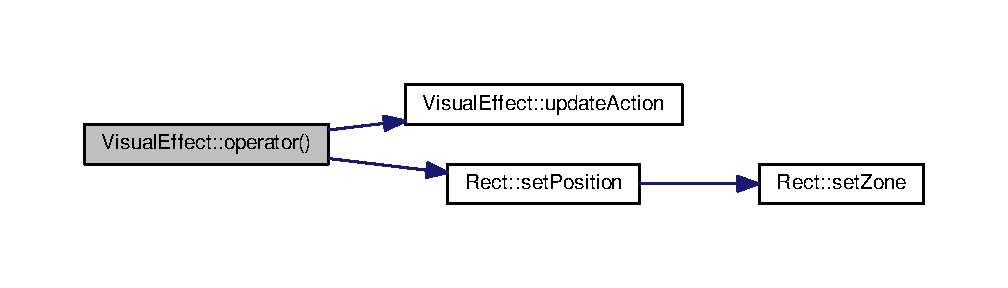
\includegraphics[width=350pt]{class_visual_effect_a8444177403c955aa02d6e82e55e34297_cgraph}
\end{center}
\end{figure}


\hypertarget{class_visual_effect_adcc6e6f9398d40e7cb9cae9edfcaace5}{\index{Visual\-Effect@{Visual\-Effect}!update\-Action@{update\-Action}}
\index{update\-Action@{update\-Action}!VisualEffect@{Visual\-Effect}}
\subsubsection[{update\-Action}]{\setlength{\rightskip}{0pt plus 5cm}void Visual\-Effect\-::update\-Action (
\begin{DoxyParamCaption}
\item[{int}]{cycle\-Actuel}
\end{DoxyParamCaption}
)\hspace{0.3cm}{\ttfamily [inline]}, {\ttfamily [protected]}}}\label{class_visual_effect_adcc6e6f9398d40e7cb9cae9edfcaace5}


Definition at line 45 of file Window\-Entity.\-h.



Referenced by operator()().



\subsection{Field Documentation}
\hypertarget{class_visual_effect_a46968c3c2f3ef411b19ea03edcb96f92}{\index{Visual\-Effect@{Visual\-Effect}!m\-\_\-active@{m\-\_\-active}}
\index{m\-\_\-active@{m\-\_\-active}!VisualEffect@{Visual\-Effect}}
\subsubsection[{m\-\_\-active}]{\setlength{\rightskip}{0pt plus 5cm}bool Visual\-Effect\-::m\-\_\-active =false\hspace{0.3cm}{\ttfamily [protected]}}}\label{class_visual_effect_a46968c3c2f3ef411b19ea03edcb96f92}


La durée d'un cycle. 



Definition at line 53 of file Window\-Entity.\-h.



Referenced by operator()().

\hypertarget{class_visual_effect_a9b414b1c6acfebad5d33a6b767c45ff7}{\index{Visual\-Effect@{Visual\-Effect}!m\-\_\-cycle\-Duration@{m\-\_\-cycle\-Duration}}
\index{m\-\_\-cycle\-Duration@{m\-\_\-cycle\-Duration}!VisualEffect@{Visual\-Effect}}
\subsubsection[{m\-\_\-cycle\-Duration}]{\setlength{\rightskip}{0pt plus 5cm}sf\-::\-Time Visual\-Effect\-::m\-\_\-cycle\-Duration\hspace{0.3cm}{\ttfamily [protected]}}}\label{class_visual_effect_a9b414b1c6acfebad5d33a6b767c45ff7}


Definition at line 51 of file Window\-Entity.\-h.



Referenced by operator()(), and Visual\-Effect().

\hypertarget{class_visual_effect_abb44ecb249d5fca2af1ecd72c5a20e49}{\index{Visual\-Effect@{Visual\-Effect}!m\-\_\-duration@{m\-\_\-duration}}
\index{m\-\_\-duration@{m\-\_\-duration}!VisualEffect@{Visual\-Effect}}
\subsubsection[{m\-\_\-duration}]{\setlength{\rightskip}{0pt plus 5cm}sf\-::\-Time Visual\-Effect\-::m\-\_\-duration\hspace{0.3cm}{\ttfamily [protected]}}}\label{class_visual_effect_abb44ecb249d5fca2af1ecd72c5a20e49}


Definition at line 50 of file Window\-Entity.\-h.



Referenced by Visual\-Effect().

\hypertarget{class_visual_effect_a345e31dcd679c46231bb028f4eb716fd}{\index{Visual\-Effect@{Visual\-Effect}!m\-\_\-remote@{m\-\_\-remote}}
\index{m\-\_\-remote@{m\-\_\-remote}!VisualEffect@{Visual\-Effect}}
\subsubsection[{m\-\_\-remote}]{\setlength{\rightskip}{0pt plus 5cm}{\bf Remote} Visual\-Effect\-::m\-\_\-remote =Remote\-::\-Continue\hspace{0.3cm}{\ttfamily [protected]}}}\label{class_visual_effect_a345e31dcd679c46231bb028f4eb716fd}


Definition at line 47 of file Window\-Entity.\-h.



Referenced by operator()().

\hypertarget{class_visual_effect_a810d29aed760dcfe3b1bd6e0fd85243a}{\index{Visual\-Effect@{Visual\-Effect}!m\-\_\-timer@{m\-\_\-timer}}
\index{m\-\_\-timer@{m\-\_\-timer}!VisualEffect@{Visual\-Effect}}
\subsubsection[{m\-\_\-timer}]{\setlength{\rightskip}{0pt plus 5cm}{\bf Timer} Visual\-Effect\-::m\-\_\-timer\hspace{0.3cm}{\ttfamily [protected]}}}\label{class_visual_effect_a810d29aed760dcfe3b1bd6e0fd85243a}


Definition at line 49 of file Window\-Entity.\-h.



Referenced by operator()().



The documentation for this class was generated from the following files\-:\begin{DoxyCompactItemize}
\item 
src/\-Graphics/\hyperlink{_window_entity_8h}{Window\-Entity.\-h}\item 
src/\-Graphics/\hyperlink{_window_entity_8cpp}{Window\-Entity.\-cpp}\end{DoxyCompactItemize}

\hypertarget{class_window_entity}{\section{Window\-Entity Class Reference}
\label{class_window_entity}\index{Window\-Entity@{Window\-Entity}}
}


{\ttfamily \#include $<$Window\-Entity.\-h$>$}



Inheritance diagram for Window\-Entity\-:\nopagebreak
\begin{figure}[H]
\begin{center}
\leavevmode
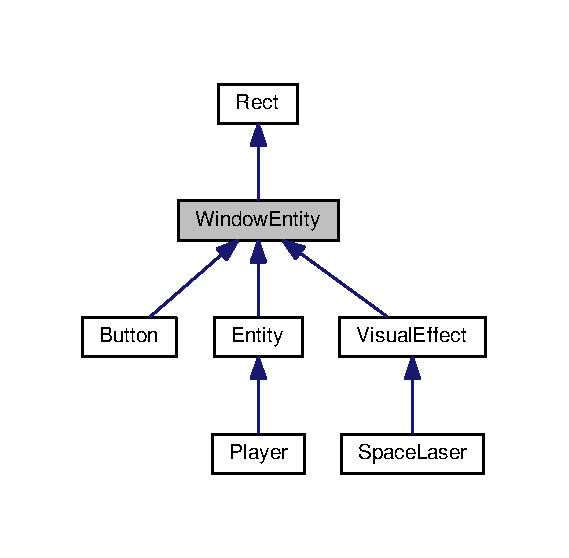
\includegraphics[width=273pt]{class_window_entity__inherit__graph}
\end{center}
\end{figure}


Collaboration diagram for Window\-Entity\-:\nopagebreak
\begin{figure}[H]
\begin{center}
\leavevmode
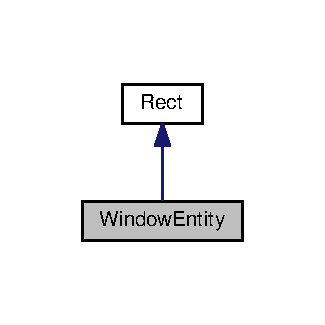
\includegraphics[width=156pt]{class_window_entity__coll__graph}
\end{center}
\end{figure}
\subsection*{Public Member Functions}
\begin{DoxyCompactItemize}
\item 
\hyperlink{class_window_entity_a71a1caf18fda6493100336a84bf62715}{Window\-Entity} ()
\item 
\hyperlink{class_window_entity_a13def047f2a274c96d5d5392c3787dca}{Window\-Entity} (std\-::string name, unsigned int priority, std\-::string texture\-I\-D=\char`\"{}\char`\"{})
\item 
void \hyperlink{class_window_entity_a1574c223b3dab59a901b7f4f2fce95c1}{load\-From\-Instructions} (std\-::string instruction\-String)
\item 
void \hyperlink{class_window_entity_aaad393d6c9f9f39266f300d930b4cebd}{add\-Texture} (std\-::string texture\-I\-D)
\item 
void \hyperlink{class_window_entity_a7756c27b2bb7edf5d6a8675675e53669}{hide\-Sprite} (int sprite=-\/1)
\item 
void \hyperlink{class_window_entity_a4e377286a13d516ffa05abbb66d9515c}{show\-Sprite} (int sprite=-\/1)
\item 
void \hyperlink{class_window_entity_afc0ddfdb22e1032751913af734025f2c}{set\-Zone} (float new\-Pos\-X, float new\-Pos\-Y, float new\-Width=0, float new\-Height=0)
\item 
void \hyperlink{class_window_entity_a9769fb7a09f6b038234b5d7937209307}{set\-Actuals} (int sprite=-\/1, int texture=0)
\begin{DoxyCompactList}\small\item\em Par défaut, cette fonction crée un nouveau sprite, sinon elle sélectionne ceux demandés. \end{DoxyCompactList}\item 
std\-::string \hyperlink{class_window_entity_a0073a5b9c6d678b090a6b8b6b10c32e3}{get\-Name} ()
\end{DoxyCompactItemize}
\subsection*{Protected Member Functions}
\begin{DoxyCompactItemize}
\item 
void \hyperlink{class_window_entity_a0f0f574a7c5ceb5abbe939388fbb86d8}{actuate\-Sprite} ()
\end{DoxyCompactItemize}
\subsection*{Protected Attributes}
\begin{DoxyCompactItemize}
\item 
sf\-::\-Sprite $\ast$ \hyperlink{class_window_entity_aa8b25adc5d948d7f52dcb3bb77e0456d}{m\-\_\-actual\-Sprite} =nullptr
\item 
sf\-::\-Texture $\ast$ \hyperlink{class_window_entity_aaceac80c2c563570032d74baed00d005}{m\-\_\-actual\-Texture} =nullptr
\item 
std\-::vector$<$ sf\-::\-Sprite $\ast$ $>$ \hyperlink{class_window_entity_aee3783d95265718dadb89afa15974d3a}{m\-\_\-sprites}
\item 
std\-::vector$<$ sf\-::\-Texture $\ast$ $>$ \hyperlink{class_window_entity_a253dbb3c77532a8a737f4cee7e7c5c81}{m\-\_\-textures}
\item 
std\-::string \hyperlink{class_window_entity_ae68db7c5aa5f1ad95a6c60091db3d441}{m\-\_\-name} =\char`\"{}Robert Paulson\char`\"{}
\item 
unsigned int \hyperlink{class_window_entity_a5903868e7d02e6e5b042a29f0b77f326}{m\-\_\-priority} =\hyperlink{general_8h_ac4b828e74900546129949acc44192072}{P\-R\-I\-O\-R\-I\-T\-Y\-\_\-\-C\-E\-N\-T\-E\-R}
\end{DoxyCompactItemize}


\subsection{Detailed Description}


Definition at line 7 of file Window\-Entity.\-h.



\subsection{Constructor \& Destructor Documentation}
\hypertarget{class_window_entity_a71a1caf18fda6493100336a84bf62715}{\index{Window\-Entity@{Window\-Entity}!Window\-Entity@{Window\-Entity}}
\index{Window\-Entity@{Window\-Entity}!WindowEntity@{Window\-Entity}}
\subsubsection[{Window\-Entity}]{\setlength{\rightskip}{0pt plus 5cm}Window\-Entity\-::\-Window\-Entity (
\begin{DoxyParamCaption}
{}
\end{DoxyParamCaption}
)}}\label{class_window_entity_a71a1caf18fda6493100336a84bf62715}


Definition at line 7 of file Window\-Entity.\-cpp.

\hypertarget{class_window_entity_a13def047f2a274c96d5d5392c3787dca}{\index{Window\-Entity@{Window\-Entity}!Window\-Entity@{Window\-Entity}}
\index{Window\-Entity@{Window\-Entity}!WindowEntity@{Window\-Entity}}
\subsubsection[{Window\-Entity}]{\setlength{\rightskip}{0pt plus 5cm}Window\-Entity\-::\-Window\-Entity (
\begin{DoxyParamCaption}
\item[{std\-::string}]{name, }
\item[{unsigned int}]{priority, }
\item[{std\-::string}]{texture\-I\-D = {\ttfamily \char`\"{}\char`\"{}}}
\end{DoxyParamCaption}
)}}\label{class_window_entity_a13def047f2a274c96d5d5392c3787dca}


Definition at line 12 of file Window\-Entity.\-cpp.



Here is the call graph for this function\-:\nopagebreak
\begin{figure}[H]
\begin{center}
\leavevmode
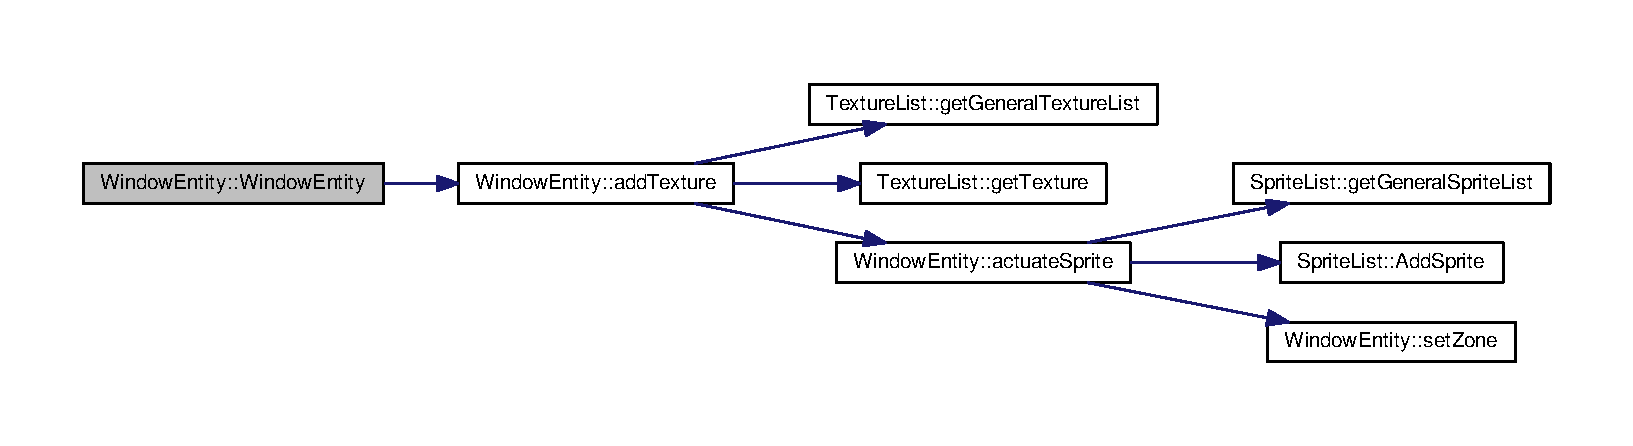
\includegraphics[width=350pt]{class_window_entity_a13def047f2a274c96d5d5392c3787dca_cgraph}
\end{center}
\end{figure}




\subsection{Member Function Documentation}
\hypertarget{class_window_entity_a0f0f574a7c5ceb5abbe939388fbb86d8}{\index{Window\-Entity@{Window\-Entity}!actuate\-Sprite@{actuate\-Sprite}}
\index{actuate\-Sprite@{actuate\-Sprite}!WindowEntity@{Window\-Entity}}
\subsubsection[{actuate\-Sprite}]{\setlength{\rightskip}{0pt plus 5cm}void Window\-Entity\-::actuate\-Sprite (
\begin{DoxyParamCaption}
{}
\end{DoxyParamCaption}
)\hspace{0.3cm}{\ttfamily [protected]}}}\label{class_window_entity_a0f0f574a7c5ceb5abbe939388fbb86d8}
\begin{DoxyNote}{Note}
check 1 
\end{DoxyNote}


Definition at line 64 of file Window\-Entity.\-cpp.



Referenced by add\-Texture().



Here is the call graph for this function\-:\nopagebreak
\begin{figure}[H]
\begin{center}
\leavevmode
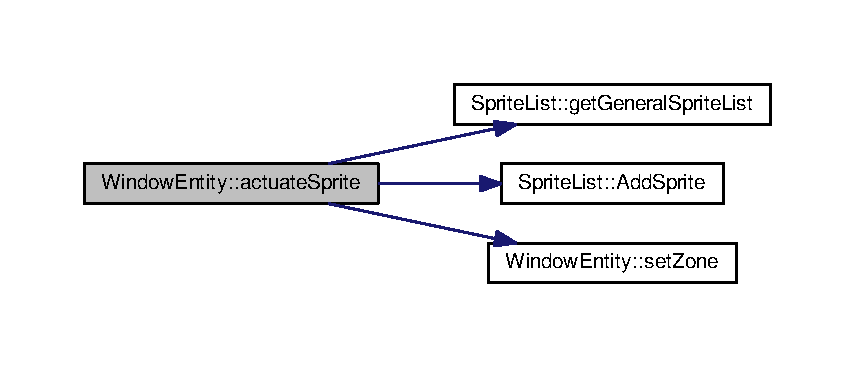
\includegraphics[width=350pt]{class_window_entity_a0f0f574a7c5ceb5abbe939388fbb86d8_cgraph}
\end{center}
\end{figure}


\hypertarget{class_window_entity_aaad393d6c9f9f39266f300d930b4cebd}{\index{Window\-Entity@{Window\-Entity}!add\-Texture@{add\-Texture}}
\index{add\-Texture@{add\-Texture}!WindowEntity@{Window\-Entity}}
\subsubsection[{add\-Texture}]{\setlength{\rightskip}{0pt plus 5cm}void Window\-Entity\-::add\-Texture (
\begin{DoxyParamCaption}
\item[{std\-::string}]{texture\-I\-D}
\end{DoxyParamCaption}
)}}\label{class_window_entity_aaad393d6c9f9f39266f300d930b4cebd}


Definition at line 83 of file Window\-Entity.\-cpp.



Referenced by load\-From\-Instructions(), and Window\-Entity().



Here is the call graph for this function\-:\nopagebreak
\begin{figure}[H]
\begin{center}
\leavevmode
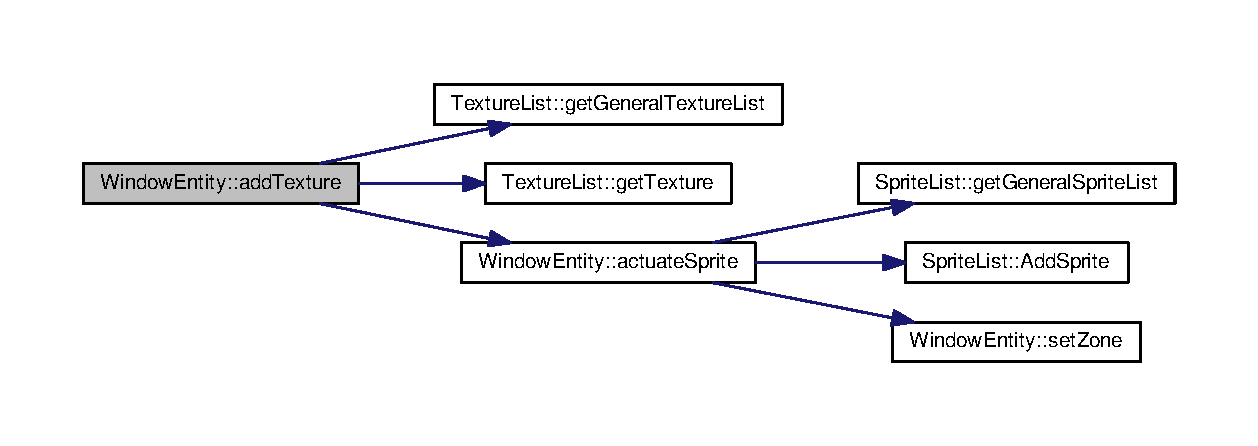
\includegraphics[width=350pt]{class_window_entity_aaad393d6c9f9f39266f300d930b4cebd_cgraph}
\end{center}
\end{figure}


\hypertarget{class_window_entity_a0073a5b9c6d678b090a6b8b6b10c32e3}{\index{Window\-Entity@{Window\-Entity}!get\-Name@{get\-Name}}
\index{get\-Name@{get\-Name}!WindowEntity@{Window\-Entity}}
\subsubsection[{get\-Name}]{\setlength{\rightskip}{0pt plus 5cm}std\-::string Window\-Entity\-::get\-Name (
\begin{DoxyParamCaption}
{}
\end{DoxyParamCaption}
)\hspace{0.3cm}{\ttfamily [inline]}}}\label{class_window_entity_a0073a5b9c6d678b090a6b8b6b10c32e3}


Definition at line 20 of file Window\-Entity.\-h.



Referenced by Ntsa\-Window\-::add\-Button().

\hypertarget{class_window_entity_a7756c27b2bb7edf5d6a8675675e53669}{\index{Window\-Entity@{Window\-Entity}!hide\-Sprite@{hide\-Sprite}}
\index{hide\-Sprite@{hide\-Sprite}!WindowEntity@{Window\-Entity}}
\subsubsection[{hide\-Sprite}]{\setlength{\rightskip}{0pt plus 5cm}void Window\-Entity\-::hide\-Sprite (
\begin{DoxyParamCaption}
\item[{int}]{sprite = {\ttfamily -\/1}}
\end{DoxyParamCaption}
)}}\label{class_window_entity_a7756c27b2bb7edf5d6a8675675e53669}
\hypertarget{class_window_entity_a1574c223b3dab59a901b7f4f2fce95c1}{\index{Window\-Entity@{Window\-Entity}!load\-From\-Instructions@{load\-From\-Instructions}}
\index{load\-From\-Instructions@{load\-From\-Instructions}!WindowEntity@{Window\-Entity}}
\subsubsection[{load\-From\-Instructions}]{\setlength{\rightskip}{0pt plus 5cm}void Window\-Entity\-::load\-From\-Instructions (
\begin{DoxyParamCaption}
\item[{std\-::string}]{instruction\-String}
\end{DoxyParamCaption}
)}}\label{class_window_entity_a1574c223b3dab59a901b7f4f2fce95c1}
\begin{DoxyRefDesc}{Todo}
\item[\hyperlink{todo__todo000001}{Todo}]Interpréter les strings comme des entiers pour priority \end{DoxyRefDesc}


Definition at line 21 of file Window\-Entity.\-cpp.



Here is the call graph for this function\-:\nopagebreak
\begin{figure}[H]
\begin{center}
\leavevmode
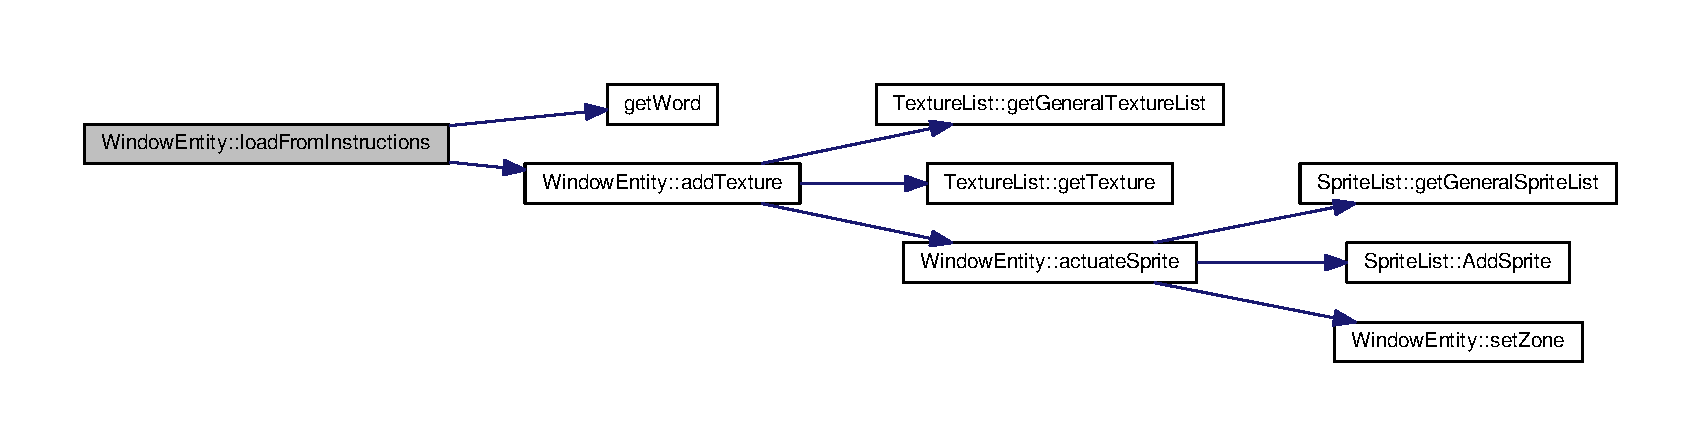
\includegraphics[width=350pt]{class_window_entity_a1574c223b3dab59a901b7f4f2fce95c1_cgraph}
\end{center}
\end{figure}


\hypertarget{class_window_entity_a9769fb7a09f6b038234b5d7937209307}{\index{Window\-Entity@{Window\-Entity}!set\-Actuals@{set\-Actuals}}
\index{set\-Actuals@{set\-Actuals}!WindowEntity@{Window\-Entity}}
\subsubsection[{set\-Actuals}]{\setlength{\rightskip}{0pt plus 5cm}void Window\-Entity\-::set\-Actuals (
\begin{DoxyParamCaption}
\item[{int}]{sprite = {\ttfamily -\/1}, }
\item[{int}]{texture = {\ttfamily 0}}
\end{DoxyParamCaption}
)}}\label{class_window_entity_a9769fb7a09f6b038234b5d7937209307}


Par défaut, cette fonction crée un nouveau sprite, sinon elle sélectionne ceux demandés. 



Definition at line 97 of file Window\-Entity.\-cpp.

\hypertarget{class_window_entity_afc0ddfdb22e1032751913af734025f2c}{\index{Window\-Entity@{Window\-Entity}!set\-Zone@{set\-Zone}}
\index{set\-Zone@{set\-Zone}!WindowEntity@{Window\-Entity}}
\subsubsection[{set\-Zone}]{\setlength{\rightskip}{0pt plus 5cm}void Window\-Entity\-::set\-Zone (
\begin{DoxyParamCaption}
\item[{float}]{new\-Pos\-X, }
\item[{float}]{new\-Pos\-Y, }
\item[{float}]{new\-Width = {\ttfamily 0}, }
\item[{float}]{new\-Height = {\ttfamily 0}}
\end{DoxyParamCaption}
)}}\label{class_window_entity_afc0ddfdb22e1032751913af734025f2c}
\begin{DoxyNote}{Note}
Check 1 
\end{DoxyNote}


Definition at line 48 of file Window\-Entity.\-cpp.



Referenced by actuate\-Sprite(), Button\-::\-Button(), and Player\-::\-Player().

\hypertarget{class_window_entity_a4e377286a13d516ffa05abbb66d9515c}{\index{Window\-Entity@{Window\-Entity}!show\-Sprite@{show\-Sprite}}
\index{show\-Sprite@{show\-Sprite}!WindowEntity@{Window\-Entity}}
\subsubsection[{show\-Sprite}]{\setlength{\rightskip}{0pt plus 5cm}void Window\-Entity\-::show\-Sprite (
\begin{DoxyParamCaption}
\item[{int}]{sprite = {\ttfamily -\/1}}
\end{DoxyParamCaption}
)}}\label{class_window_entity_a4e377286a13d516ffa05abbb66d9515c}


\subsection{Field Documentation}
\hypertarget{class_window_entity_aa8b25adc5d948d7f52dcb3bb77e0456d}{\index{Window\-Entity@{Window\-Entity}!m\-\_\-actual\-Sprite@{m\-\_\-actual\-Sprite}}
\index{m\-\_\-actual\-Sprite@{m\-\_\-actual\-Sprite}!WindowEntity@{Window\-Entity}}
\subsubsection[{m\-\_\-actual\-Sprite}]{\setlength{\rightskip}{0pt plus 5cm}sf\-::\-Sprite$\ast$ Window\-Entity\-::m\-\_\-actual\-Sprite =nullptr\hspace{0.3cm}{\ttfamily [protected]}}}\label{class_window_entity_aa8b25adc5d948d7f52dcb3bb77e0456d}


Definition at line 25 of file Window\-Entity.\-h.



Referenced by actuate\-Sprite(), set\-Actuals(), and set\-Zone().

\hypertarget{class_window_entity_aaceac80c2c563570032d74baed00d005}{\index{Window\-Entity@{Window\-Entity}!m\-\_\-actual\-Texture@{m\-\_\-actual\-Texture}}
\index{m\-\_\-actual\-Texture@{m\-\_\-actual\-Texture}!WindowEntity@{Window\-Entity}}
\subsubsection[{m\-\_\-actual\-Texture}]{\setlength{\rightskip}{0pt plus 5cm}sf\-::\-Texture$\ast$ Window\-Entity\-::m\-\_\-actual\-Texture =nullptr\hspace{0.3cm}{\ttfamily [protected]}}}\label{class_window_entity_aaceac80c2c563570032d74baed00d005}


Definition at line 26 of file Window\-Entity.\-h.



Referenced by actuate\-Sprite(), add\-Texture(), and set\-Actuals().

\hypertarget{class_window_entity_ae68db7c5aa5f1ad95a6c60091db3d441}{\index{Window\-Entity@{Window\-Entity}!m\-\_\-name@{m\-\_\-name}}
\index{m\-\_\-name@{m\-\_\-name}!WindowEntity@{Window\-Entity}}
\subsubsection[{m\-\_\-name}]{\setlength{\rightskip}{0pt plus 5cm}std\-::string Window\-Entity\-::m\-\_\-name =\char`\"{}Robert Paulson\char`\"{}\hspace{0.3cm}{\ttfamily [protected]}}}\label{class_window_entity_ae68db7c5aa5f1ad95a6c60091db3d441}


Definition at line 31 of file Window\-Entity.\-h.



Referenced by actuate\-Sprite(), add\-Texture(), get\-Name(), and load\-From\-Instructions().

\hypertarget{class_window_entity_a5903868e7d02e6e5b042a29f0b77f326}{\index{Window\-Entity@{Window\-Entity}!m\-\_\-priority@{m\-\_\-priority}}
\index{m\-\_\-priority@{m\-\_\-priority}!WindowEntity@{Window\-Entity}}
\subsubsection[{m\-\_\-priority}]{\setlength{\rightskip}{0pt plus 5cm}unsigned int Window\-Entity\-::m\-\_\-priority ={\bf P\-R\-I\-O\-R\-I\-T\-Y\-\_\-\-C\-E\-N\-T\-E\-R}\hspace{0.3cm}{\ttfamily [protected]}}}\label{class_window_entity_a5903868e7d02e6e5b042a29f0b77f326}


Definition at line 32 of file Window\-Entity.\-h.



Referenced by actuate\-Sprite(), and load\-From\-Instructions().

\hypertarget{class_window_entity_aee3783d95265718dadb89afa15974d3a}{\index{Window\-Entity@{Window\-Entity}!m\-\_\-sprites@{m\-\_\-sprites}}
\index{m\-\_\-sprites@{m\-\_\-sprites}!WindowEntity@{Window\-Entity}}
\subsubsection[{m\-\_\-sprites}]{\setlength{\rightskip}{0pt plus 5cm}std\-::vector$<$sf\-::\-Sprite$\ast$$>$ Window\-Entity\-::m\-\_\-sprites\hspace{0.3cm}{\ttfamily [protected]}}}\label{class_window_entity_aee3783d95265718dadb89afa15974d3a}


Definition at line 28 of file Window\-Entity.\-h.



Referenced by actuate\-Sprite(), Visual\-Effect\-::operator()(), and set\-Actuals().

\hypertarget{class_window_entity_a253dbb3c77532a8a737f4cee7e7c5c81}{\index{Window\-Entity@{Window\-Entity}!m\-\_\-textures@{m\-\_\-textures}}
\index{m\-\_\-textures@{m\-\_\-textures}!WindowEntity@{Window\-Entity}}
\subsubsection[{m\-\_\-textures}]{\setlength{\rightskip}{0pt plus 5cm}std\-::vector$<$sf\-::\-Texture$\ast$$>$ Window\-Entity\-::m\-\_\-textures\hspace{0.3cm}{\ttfamily [protected]}}}\label{class_window_entity_a253dbb3c77532a8a737f4cee7e7c5c81}


Definition at line 29 of file Window\-Entity.\-h.



Referenced by add\-Texture(), and set\-Actuals().



The documentation for this class was generated from the following files\-:\begin{DoxyCompactItemize}
\item 
src/\-Graphics/\hyperlink{_window_entity_8h}{Window\-Entity.\-h}\item 
src/\-Graphics/\hyperlink{_window_entity_8cpp}{Window\-Entity.\-cpp}\end{DoxyCompactItemize}

\chapter{File Documentation}
\input{_core_2_u_i_8cpp}
\input{_graphics_2_u_i_8cpp}
\input{_core_2_u_i_8h}
\input{_graphics_2_u_i_8h}
\hypertarget{general_8cpp}{\section{src/\-General/general.cpp File Reference}
\label{general_8cpp}\index{src/\-General/general.\-cpp@{src/\-General/general.\-cpp}}
}
{\ttfamily \#include \char`\"{}../\-General/general.\-h\char`\"{}}\\*
Include dependency graph for general.\-cpp\-:\nopagebreak
\begin{figure}[H]
\begin{center}
\leavevmode
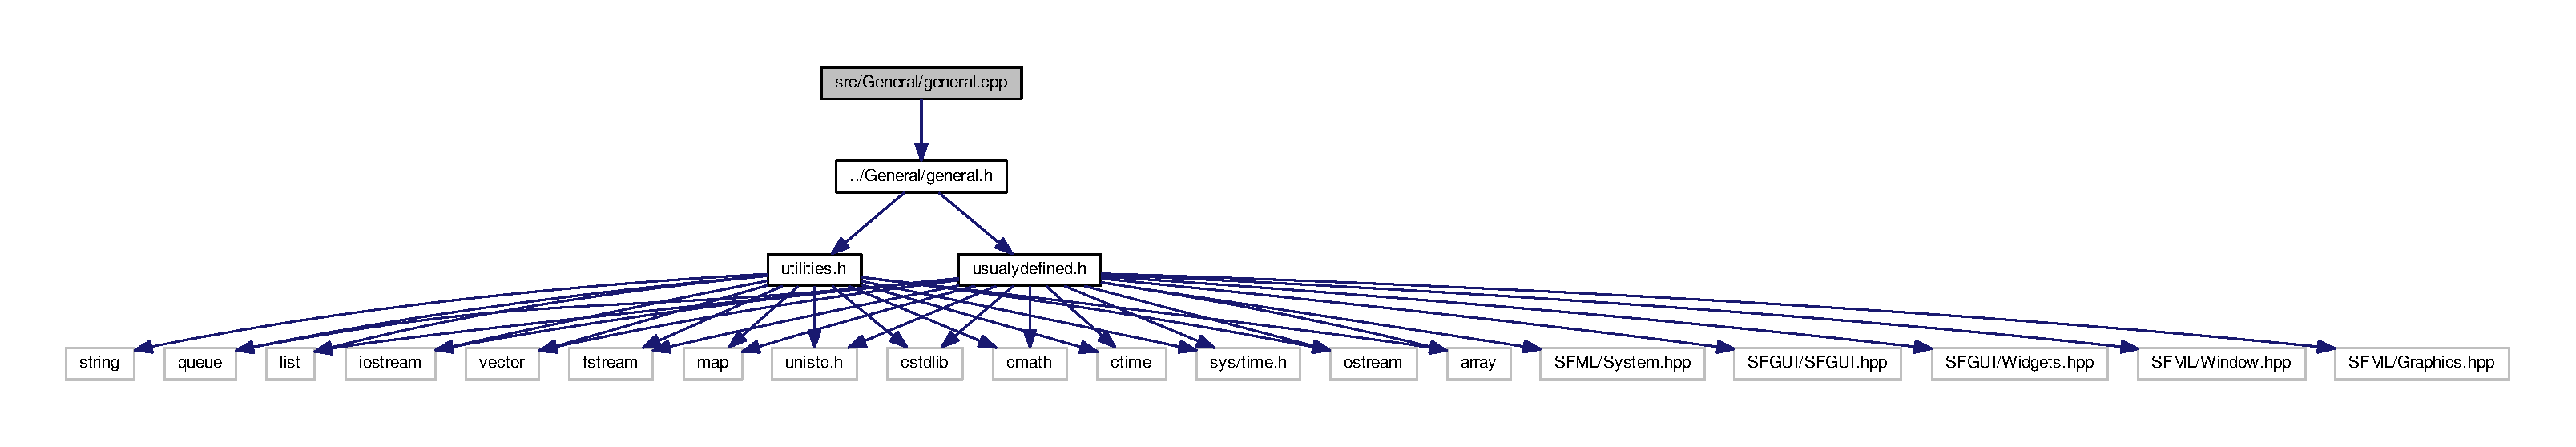
\includegraphics[width=350pt]{general_8cpp__incl}
\end{center}
\end{figure}
\subsection*{Variables}
\begin{DoxyCompactItemize}
\item 
\hyperlink{class_sprite_list}{Sprite\-List} \hyperlink{general_8cpp_a36687f7e9c02107fffc4f48f4ba77d65}{general\-Sprite\-List}
\item 
\hyperlink{class_texture_list}{Texture\-List} \hyperlink{general_8cpp_a3be1d11c93e7fbe1e30fc437d8b772b3}{general\-Texture\-List}
\end{DoxyCompactItemize}


\subsection{Variable Documentation}
\hypertarget{general_8cpp_a36687f7e9c02107fffc4f48f4ba77d65}{\index{general.\-cpp@{general.\-cpp}!general\-Sprite\-List@{general\-Sprite\-List}}
\index{general\-Sprite\-List@{general\-Sprite\-List}!general.cpp@{general.\-cpp}}
\subsubsection[{general\-Sprite\-List}]{\setlength{\rightskip}{0pt plus 5cm}{\bf Sprite\-List} general\-Sprite\-List}}\label{general_8cpp_a36687f7e9c02107fffc4f48f4ba77d65}


Definition at line 4 of file general.\-cpp.



Referenced by Sprite\-List\-::get\-General\-Sprite\-List().

\hypertarget{general_8cpp_a3be1d11c93e7fbe1e30fc437d8b772b3}{\index{general.\-cpp@{general.\-cpp}!general\-Texture\-List@{general\-Texture\-List}}
\index{general\-Texture\-List@{general\-Texture\-List}!general.cpp@{general.\-cpp}}
\subsubsection[{general\-Texture\-List}]{\setlength{\rightskip}{0pt plus 5cm}{\bf Texture\-List} general\-Texture\-List}}\label{general_8cpp_a3be1d11c93e7fbe1e30fc437d8b772b3}


Definition at line 5 of file general.\-cpp.



Referenced by Texture\-List\-::get\-General\-Texture\-List().


\hypertarget{general_8h}{\section{src/\-General/general.h File Reference}
\label{general_8h}\index{src/\-General/general.\-h@{src/\-General/general.\-h}}
}
{\ttfamily \#include \char`\"{}usualydefined.\-h\char`\"{}}\\*
{\ttfamily \#include \char`\"{}utilities.\-h\char`\"{}}\\*
Include dependency graph for general.\-h\-:\nopagebreak
\begin{figure}[H]
\begin{center}
\leavevmode
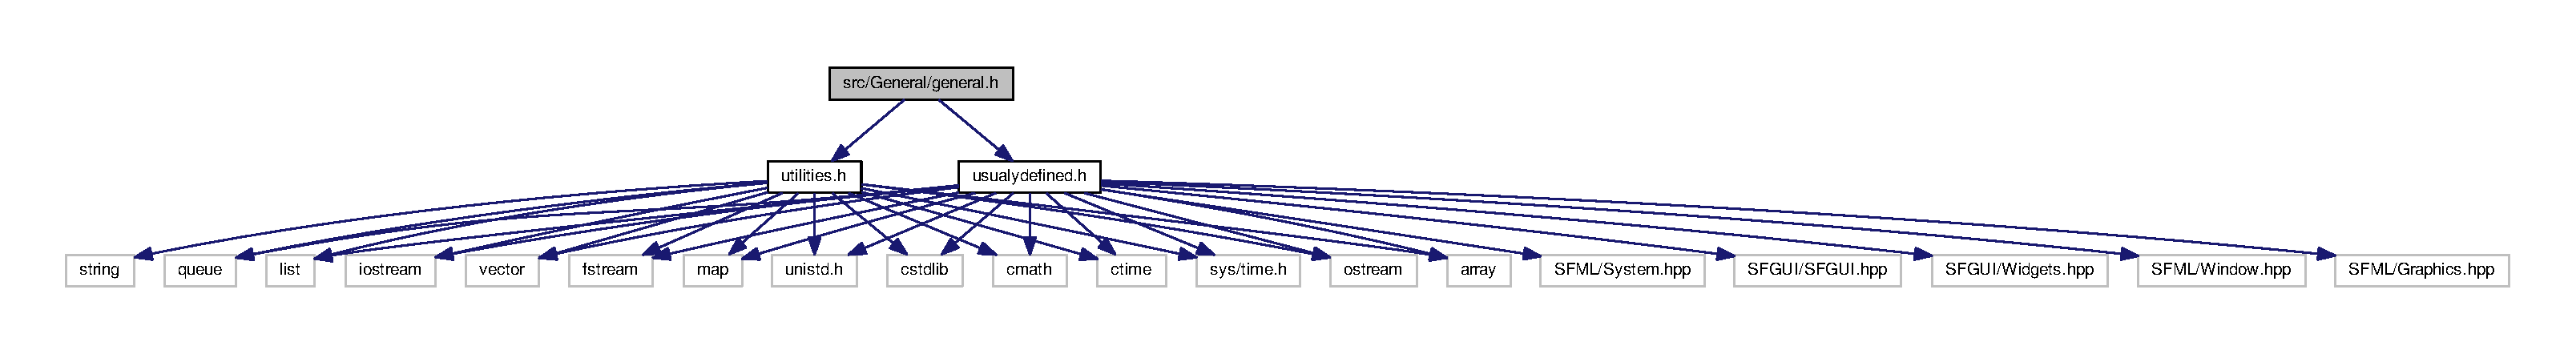
\includegraphics[width=350pt]{general_8h__incl}
\end{center}
\end{figure}
This graph shows which files directly or indirectly include this file\-:
\nopagebreak
\begin{figure}[H]
\begin{center}
\leavevmode
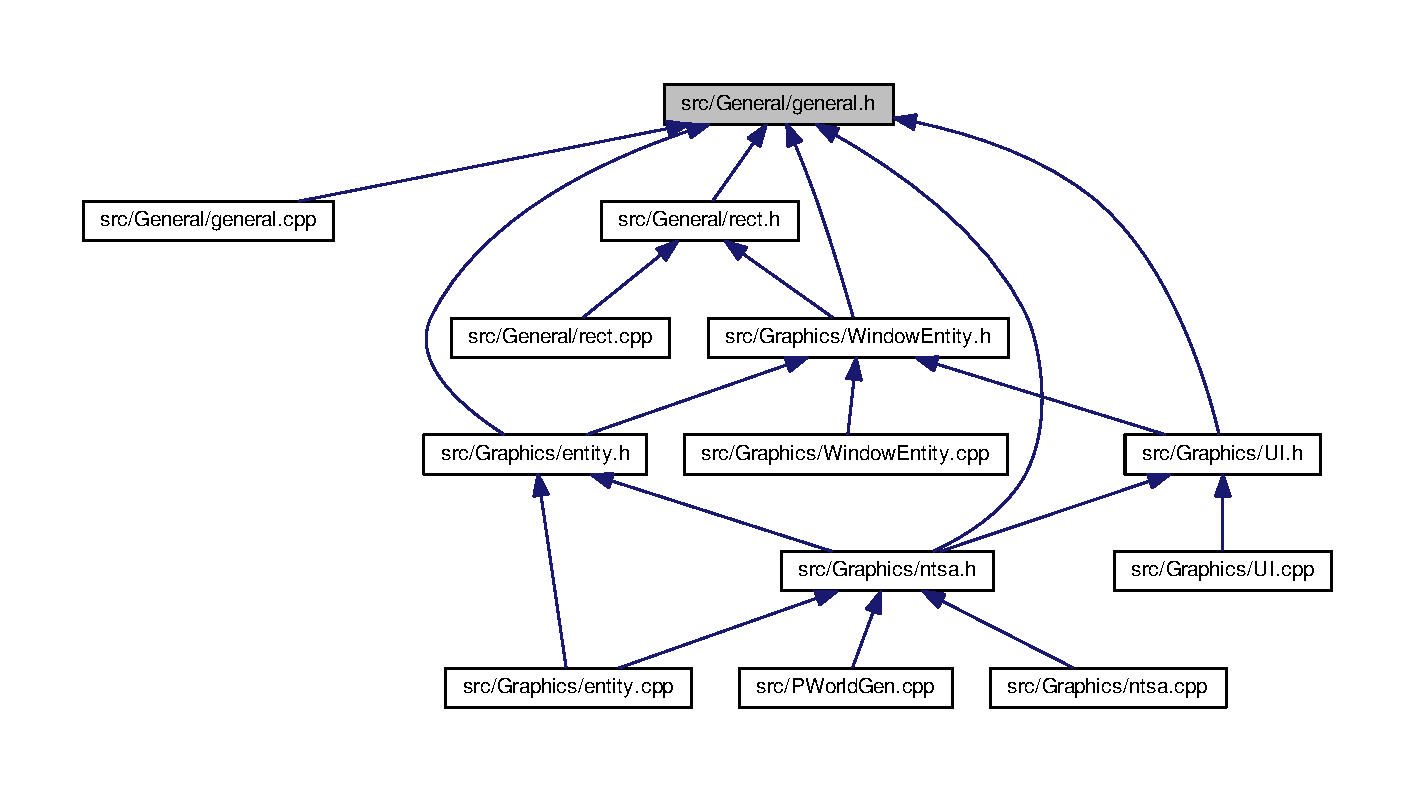
\includegraphics[width=350pt]{general_8h__dep__incl}
\end{center}
\end{figure}
\subsection*{Data Structures}
\begin{DoxyCompactItemize}
\item 
class \hyperlink{class_timer}{Timer}
\item 
class \hyperlink{class_sprite_list}{Sprite\-List}
\item 
class \hyperlink{class_texture_list}{Texture\-List}
\end{DoxyCompactItemize}
\subsection*{Macros}
\begin{DoxyCompactItemize}
\item 
\#define \hyperlink{general_8h_a8163a38b42a3799cad180b48fa23e156}{P\-R\-I\-O\-R\-I\-T\-Y\-\_\-\-B\-A\-C\-K\-G\-R\-O\-U\-N\-D0}~1000000
\item 
\#define \hyperlink{general_8h_af14e7b164610db375fe1eec0eeb641a1}{P\-R\-I\-O\-R\-I\-T\-Y\-\_\-\-B\-A\-C\-K\-G\-R\-O\-U\-N\-D1}~500000
\item 
\#define \hyperlink{general_8h_a957ec000ff4ea597a02f11b618eb00e7}{P\-R\-I\-O\-R\-I\-T\-Y\-\_\-\-B\-E\-F\-O\-R\-E\-C\-E\-N\-T\-E\-R}~100000
\item 
\#define \hyperlink{general_8h_ac4b828e74900546129949acc44192072}{P\-R\-I\-O\-R\-I\-T\-Y\-\_\-\-C\-E\-N\-T\-E\-R}~50000
\item 
\#define \hyperlink{general_8h_afe94e0bd995f71efd00cb897186e5e48}{P\-R\-I\-O\-R\-I\-T\-Y\-\_\-\-T\-O\-P}~10000
\item 
\#define \hyperlink{general_8h_a24eeca326b343ef747382e995c1611ba}{P\-R\-I\-O\-R\-I\-T\-Y\-\_\-\-T\-O\-T\-T}~1000
\end{DoxyCompactItemize}


\subsection{Macro Definition Documentation}
\hypertarget{general_8h_a8163a38b42a3799cad180b48fa23e156}{\index{general.\-h@{general.\-h}!P\-R\-I\-O\-R\-I\-T\-Y\-\_\-\-B\-A\-C\-K\-G\-R\-O\-U\-N\-D0@{P\-R\-I\-O\-R\-I\-T\-Y\-\_\-\-B\-A\-C\-K\-G\-R\-O\-U\-N\-D0}}
\index{P\-R\-I\-O\-R\-I\-T\-Y\-\_\-\-B\-A\-C\-K\-G\-R\-O\-U\-N\-D0@{P\-R\-I\-O\-R\-I\-T\-Y\-\_\-\-B\-A\-C\-K\-G\-R\-O\-U\-N\-D0}!general.h@{general.\-h}}
\subsubsection[{P\-R\-I\-O\-R\-I\-T\-Y\-\_\-\-B\-A\-C\-K\-G\-R\-O\-U\-N\-D0}]{\setlength{\rightskip}{0pt plus 5cm}\#define P\-R\-I\-O\-R\-I\-T\-Y\-\_\-\-B\-A\-C\-K\-G\-R\-O\-U\-N\-D0~1000000}}\label{general_8h_a8163a38b42a3799cad180b48fa23e156}


Definition at line 7 of file general.\-h.

\hypertarget{general_8h_af14e7b164610db375fe1eec0eeb641a1}{\index{general.\-h@{general.\-h}!P\-R\-I\-O\-R\-I\-T\-Y\-\_\-\-B\-A\-C\-K\-G\-R\-O\-U\-N\-D1@{P\-R\-I\-O\-R\-I\-T\-Y\-\_\-\-B\-A\-C\-K\-G\-R\-O\-U\-N\-D1}}
\index{P\-R\-I\-O\-R\-I\-T\-Y\-\_\-\-B\-A\-C\-K\-G\-R\-O\-U\-N\-D1@{P\-R\-I\-O\-R\-I\-T\-Y\-\_\-\-B\-A\-C\-K\-G\-R\-O\-U\-N\-D1}!general.h@{general.\-h}}
\subsubsection[{P\-R\-I\-O\-R\-I\-T\-Y\-\_\-\-B\-A\-C\-K\-G\-R\-O\-U\-N\-D1}]{\setlength{\rightskip}{0pt plus 5cm}\#define P\-R\-I\-O\-R\-I\-T\-Y\-\_\-\-B\-A\-C\-K\-G\-R\-O\-U\-N\-D1~500000}}\label{general_8h_af14e7b164610db375fe1eec0eeb641a1}


Definition at line 8 of file general.\-h.

\hypertarget{general_8h_a957ec000ff4ea597a02f11b618eb00e7}{\index{general.\-h@{general.\-h}!P\-R\-I\-O\-R\-I\-T\-Y\-\_\-\-B\-E\-F\-O\-R\-E\-C\-E\-N\-T\-E\-R@{P\-R\-I\-O\-R\-I\-T\-Y\-\_\-\-B\-E\-F\-O\-R\-E\-C\-E\-N\-T\-E\-R}}
\index{P\-R\-I\-O\-R\-I\-T\-Y\-\_\-\-B\-E\-F\-O\-R\-E\-C\-E\-N\-T\-E\-R@{P\-R\-I\-O\-R\-I\-T\-Y\-\_\-\-B\-E\-F\-O\-R\-E\-C\-E\-N\-T\-E\-R}!general.h@{general.\-h}}
\subsubsection[{P\-R\-I\-O\-R\-I\-T\-Y\-\_\-\-B\-E\-F\-O\-R\-E\-C\-E\-N\-T\-E\-R}]{\setlength{\rightskip}{0pt plus 5cm}\#define P\-R\-I\-O\-R\-I\-T\-Y\-\_\-\-B\-E\-F\-O\-R\-E\-C\-E\-N\-T\-E\-R~100000}}\label{general_8h_a957ec000ff4ea597a02f11b618eb00e7}


Definition at line 9 of file general.\-h.

\hypertarget{general_8h_ac4b828e74900546129949acc44192072}{\index{general.\-h@{general.\-h}!P\-R\-I\-O\-R\-I\-T\-Y\-\_\-\-C\-E\-N\-T\-E\-R@{P\-R\-I\-O\-R\-I\-T\-Y\-\_\-\-C\-E\-N\-T\-E\-R}}
\index{P\-R\-I\-O\-R\-I\-T\-Y\-\_\-\-C\-E\-N\-T\-E\-R@{P\-R\-I\-O\-R\-I\-T\-Y\-\_\-\-C\-E\-N\-T\-E\-R}!general.h@{general.\-h}}
\subsubsection[{P\-R\-I\-O\-R\-I\-T\-Y\-\_\-\-C\-E\-N\-T\-E\-R}]{\setlength{\rightskip}{0pt plus 5cm}\#define P\-R\-I\-O\-R\-I\-T\-Y\-\_\-\-C\-E\-N\-T\-E\-R~50000}}\label{general_8h_ac4b828e74900546129949acc44192072}


Definition at line 10 of file general.\-h.



Referenced by Window\-Entity\-::load\-From\-Instructions().

\hypertarget{general_8h_afe94e0bd995f71efd00cb897186e5e48}{\index{general.\-h@{general.\-h}!P\-R\-I\-O\-R\-I\-T\-Y\-\_\-\-T\-O\-P@{P\-R\-I\-O\-R\-I\-T\-Y\-\_\-\-T\-O\-P}}
\index{P\-R\-I\-O\-R\-I\-T\-Y\-\_\-\-T\-O\-P@{P\-R\-I\-O\-R\-I\-T\-Y\-\_\-\-T\-O\-P}!general.h@{general.\-h}}
\subsubsection[{P\-R\-I\-O\-R\-I\-T\-Y\-\_\-\-T\-O\-P}]{\setlength{\rightskip}{0pt plus 5cm}\#define P\-R\-I\-O\-R\-I\-T\-Y\-\_\-\-T\-O\-P~10000}}\label{general_8h_afe94e0bd995f71efd00cb897186e5e48}


Definition at line 11 of file general.\-h.

\hypertarget{general_8h_a24eeca326b343ef747382e995c1611ba}{\index{general.\-h@{general.\-h}!P\-R\-I\-O\-R\-I\-T\-Y\-\_\-\-T\-O\-T\-T@{P\-R\-I\-O\-R\-I\-T\-Y\-\_\-\-T\-O\-T\-T}}
\index{P\-R\-I\-O\-R\-I\-T\-Y\-\_\-\-T\-O\-T\-T@{P\-R\-I\-O\-R\-I\-T\-Y\-\_\-\-T\-O\-T\-T}!general.h@{general.\-h}}
\subsubsection[{P\-R\-I\-O\-R\-I\-T\-Y\-\_\-\-T\-O\-T\-T}]{\setlength{\rightskip}{0pt plus 5cm}\#define P\-R\-I\-O\-R\-I\-T\-Y\-\_\-\-T\-O\-T\-T~1000}}\label{general_8h_a24eeca326b343ef747382e995c1611ba}


Definition at line 12 of file general.\-h.


\hypertarget{rect_8cpp}{\section{src/\-General/rect.cpp File Reference}
\label{rect_8cpp}\index{src/\-General/rect.\-cpp@{src/\-General/rect.\-cpp}}
}
{\ttfamily \#include \char`\"{}rect.\-h\char`\"{}}\\*
Include dependency graph for rect.\-cpp\-:\nopagebreak
\begin{figure}[H]
\begin{center}
\leavevmode
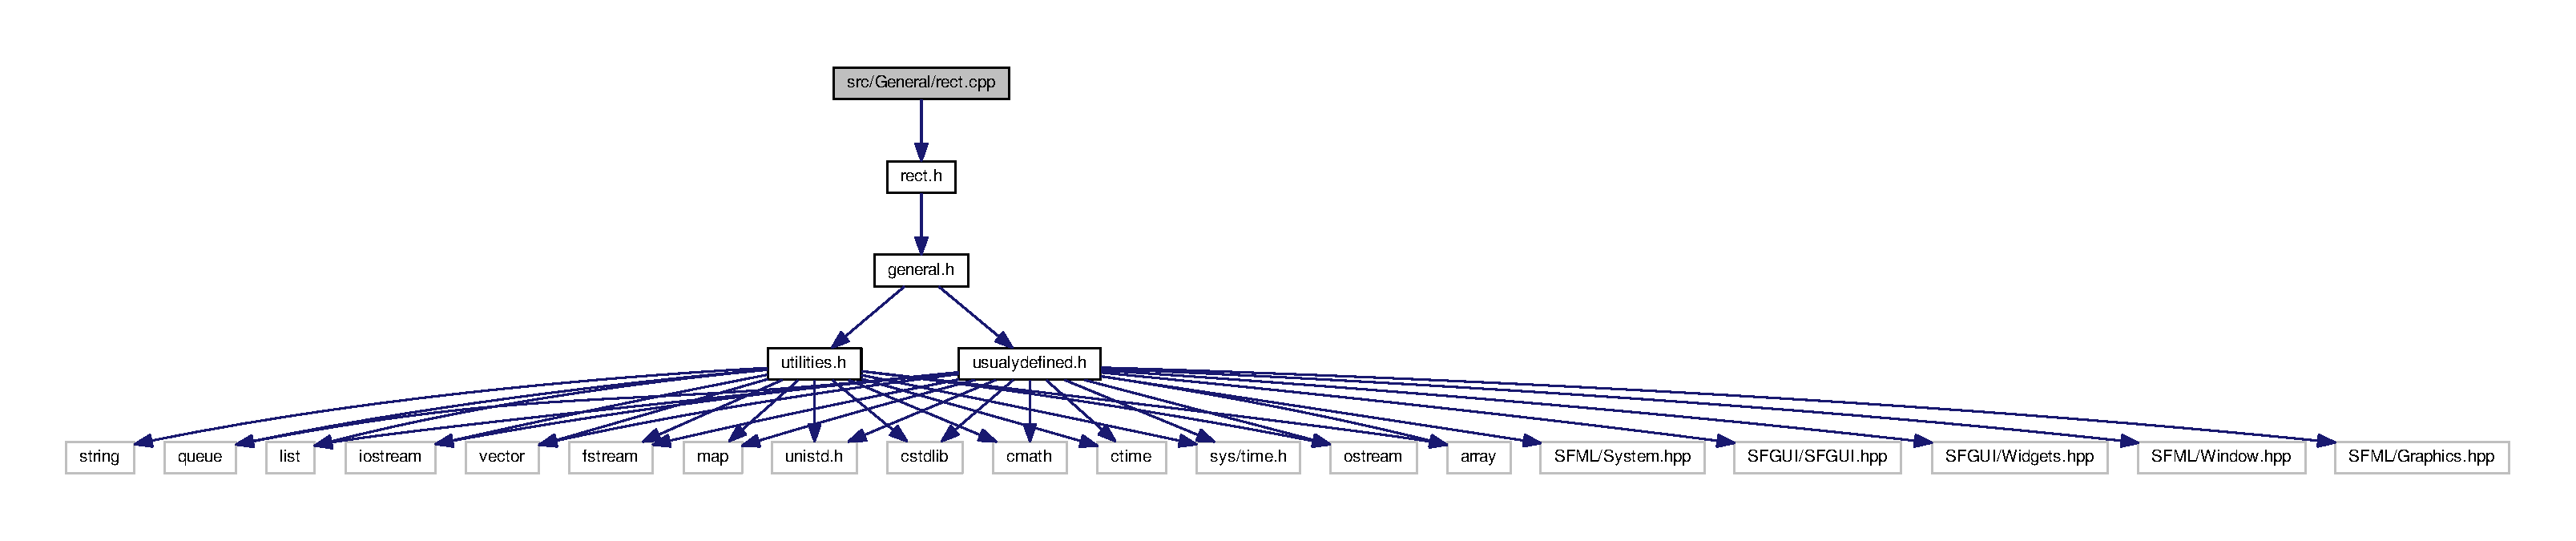
\includegraphics[width=350pt]{rect_8cpp__incl}
\end{center}
\end{figure}
\subsection*{Functions}
\begin{DoxyCompactItemize}
\item 
bool \hyperlink{rect_8cpp_a38c616798c26ba8b243898c800d04a69}{operator==} (\hyperlink{class_rect}{Rect} \&left, \hyperlink{class_rect}{Rect} \&right)
\item 
bool \hyperlink{rect_8cpp_a65bcff7eb442ac55beb0dfd9dafc0dbc}{operator!=} (const \hyperlink{class_rect}{Rect} \&m\-\_\-pos\-X, const \hyperlink{class_rect}{Rect} \&right)
\end{DoxyCompactItemize}


\subsection{Function Documentation}
\hypertarget{rect_8cpp_a65bcff7eb442ac55beb0dfd9dafc0dbc}{\index{rect.\-cpp@{rect.\-cpp}!operator!=@{operator!=}}
\index{operator!=@{operator!=}!rect.cpp@{rect.\-cpp}}
\subsubsection[{operator!=}]{\setlength{\rightskip}{0pt plus 5cm}bool operator!= (
\begin{DoxyParamCaption}
\item[{const {\bf Rect} \&}]{m\-\_\-pos\-X, }
\item[{const {\bf Rect} \&}]{right}
\end{DoxyParamCaption}
)\hspace{0.3cm}{\ttfamily [inline]}}}\label{rect_8cpp_a65bcff7eb442ac55beb0dfd9dafc0dbc}


Definition at line 136 of file rect.\-cpp.

\hypertarget{rect_8cpp_a38c616798c26ba8b243898c800d04a69}{\index{rect.\-cpp@{rect.\-cpp}!operator==@{operator==}}
\index{operator==@{operator==}!rect.cpp@{rect.\-cpp}}
\subsubsection[{operator==}]{\setlength{\rightskip}{0pt plus 5cm}bool operator== (
\begin{DoxyParamCaption}
\item[{{\bf Rect} \&}]{left, }
\item[{{\bf Rect} \&}]{right}
\end{DoxyParamCaption}
)\hspace{0.3cm}{\ttfamily [inline]}}}\label{rect_8cpp_a38c616798c26ba8b243898c800d04a69}


Definition at line 129 of file rect.\-cpp.



Here is the call graph for this function\-:\nopagebreak
\begin{figure}[H]
\begin{center}
\leavevmode
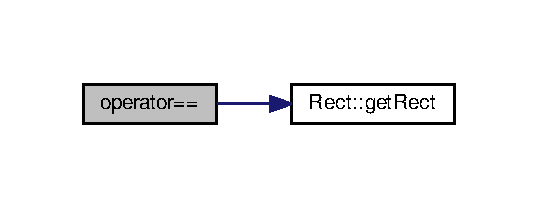
\includegraphics[width=258pt]{rect_8cpp_a38c616798c26ba8b243898c800d04a69_cgraph}
\end{center}
\end{figure}



\hypertarget{rect_8h}{\section{src/\-General/rect.h File Reference}
\label{rect_8h}\index{src/\-General/rect.\-h@{src/\-General/rect.\-h}}
}
{\ttfamily \#include \char`\"{}general.\-h\char`\"{}}\\*
Include dependency graph for rect.\-h\-:\nopagebreak
\begin{figure}[H]
\begin{center}
\leavevmode
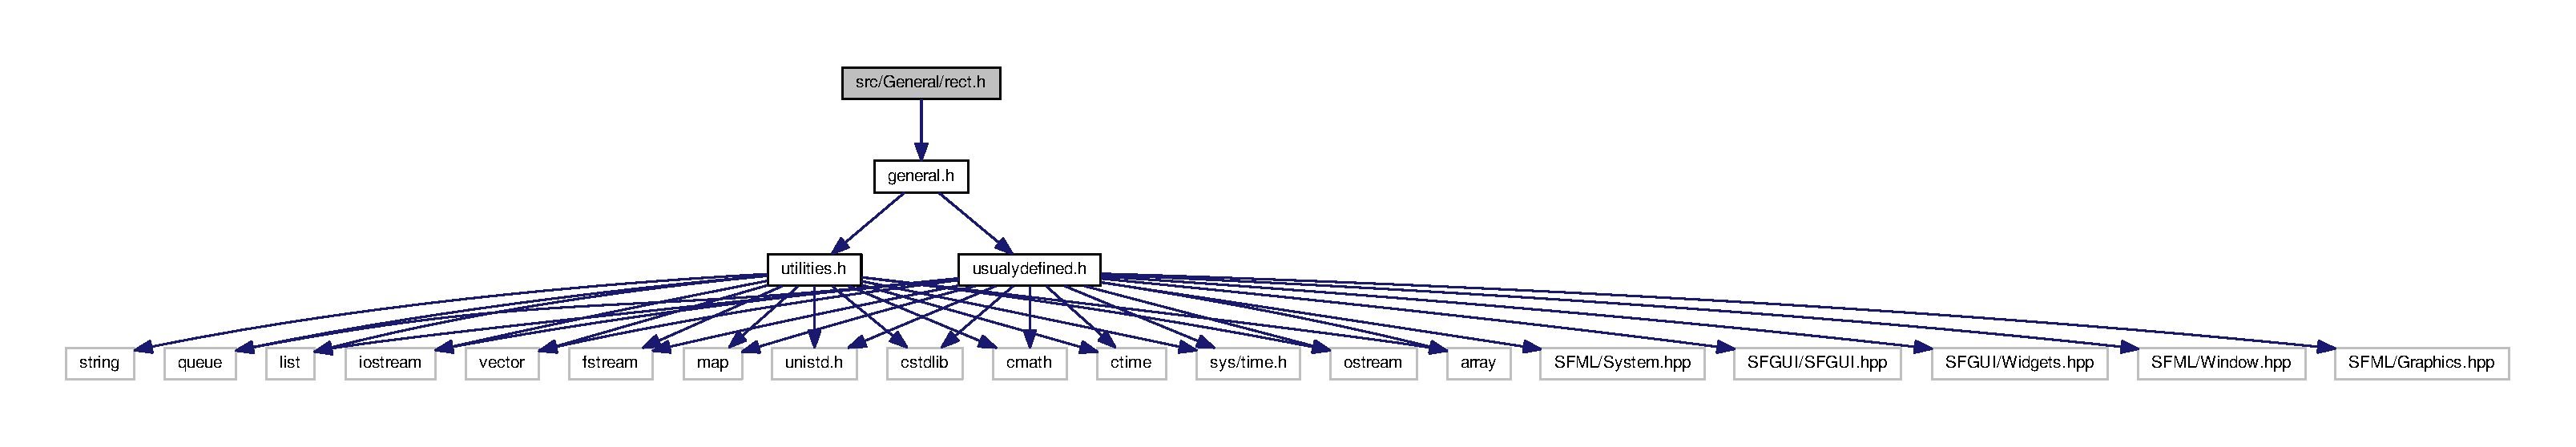
\includegraphics[width=350pt]{rect_8h__incl}
\end{center}
\end{figure}
This graph shows which files directly or indirectly include this file\-:\nopagebreak
\begin{figure}[H]
\begin{center}
\leavevmode
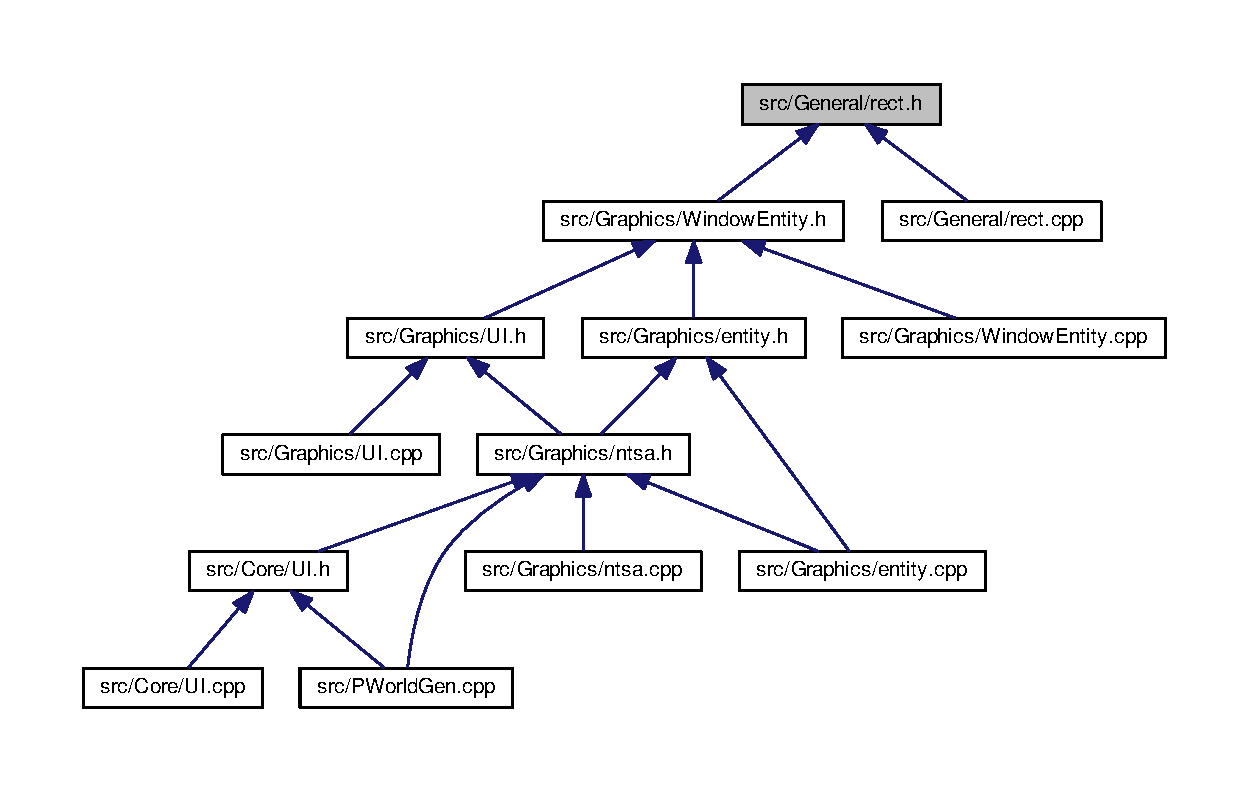
\includegraphics[width=350pt]{rect_8h__dep__incl}
\end{center}
\end{figure}
\subsection*{Data Structures}
\begin{DoxyCompactItemize}
\item 
class \hyperlink{class_public_rect}{Public\-Rect}
\item 
class \hyperlink{class_rect}{Rect}
\end{DoxyCompactItemize}
\subsection*{Functions}
\begin{DoxyCompactItemize}
\item 
bool \hyperlink{rect_8h_a4fa1ffec0624b6b7a8b5acb6b201eeaa}{operator==} (const \hyperlink{class_rect}{Rect} \&left, const \hyperlink{class_rect}{Rect} \&right)
\item 
bool \hyperlink{rect_8h_a0e88e9274a97afa04df75e678e1d881f}{operator!=} (const \hyperlink{class_rect}{Rect} \&left, const \hyperlink{class_rect}{Rect} \&right)
\end{DoxyCompactItemize}


\subsection{Function Documentation}
\hypertarget{rect_8h_a0e88e9274a97afa04df75e678e1d881f}{\index{rect.\-h@{rect.\-h}!operator!=@{operator!=}}
\index{operator!=@{operator!=}!rect.h@{rect.\-h}}
\subsubsection[{operator!=}]{\setlength{\rightskip}{0pt plus 5cm}bool operator!= (
\begin{DoxyParamCaption}
\item[{const {\bf Rect} \&}]{left, }
\item[{const {\bf Rect} \&}]{right}
\end{DoxyParamCaption}
)\hspace{0.3cm}{\ttfamily [inline]}}}\label{rect_8h_a0e88e9274a97afa04df75e678e1d881f}


Definition at line 136 of file rect.\-cpp.

\hypertarget{rect_8h_a4fa1ffec0624b6b7a8b5acb6b201eeaa}{\index{rect.\-h@{rect.\-h}!operator==@{operator==}}
\index{operator==@{operator==}!rect.h@{rect.\-h}}
\subsubsection[{operator==}]{\setlength{\rightskip}{0pt plus 5cm}bool operator== (
\begin{DoxyParamCaption}
\item[{const {\bf Rect} \&}]{left, }
\item[{const {\bf Rect} \&}]{right}
\end{DoxyParamCaption}
)}}\label{rect_8h_a4fa1ffec0624b6b7a8b5acb6b201eeaa}

\hypertarget{usualydefined_8h}{\section{src/\-General/usualydefined.h File Reference}
\label{usualydefined_8h}\index{src/\-General/usualydefined.\-h@{src/\-General/usualydefined.\-h}}
}
{\ttfamily \#include $<$iostream$>$}\\*
{\ttfamily \#include $<$vector$>$}\\*
{\ttfamily \#include $<$fstream$>$}\\*
{\ttfamily \#include $<$map$>$}\\*
{\ttfamily \#include $<$unistd.\-h$>$}\\*
{\ttfamily \#include $<$cstdlib$>$}\\*
{\ttfamily \#include $<$cmath$>$}\\*
{\ttfamily \#include $<$ctime$>$}\\*
{\ttfamily \#include $<$sys/time.\-h$>$}\\*
{\ttfamily \#include $<$ostream$>$}\\*
{\ttfamily \#include $<$array$>$}\\*
{\ttfamily \#include $<$queue$>$}\\*
{\ttfamily \#include $<$list$>$}\\*
{\ttfamily \#include $<$S\-F\-M\-L/\-Window.\-hpp$>$}\\*
{\ttfamily \#include $<$S\-F\-M\-L/\-Graphics.\-hpp$>$}\\*
{\ttfamily \#include $<$S\-F\-M\-L/\-System.\-hpp$>$}\\*
{\ttfamily \#include $<$S\-F\-G\-U\-I/\-S\-F\-G\-U\-I.\-hpp$>$}\\*
{\ttfamily \#include $<$S\-F\-G\-U\-I/\-Widgets.\-hpp$>$}\\*
Include dependency graph for usualydefined.\-h\-:\nopagebreak
\begin{figure}[H]
\begin{center}
\leavevmode
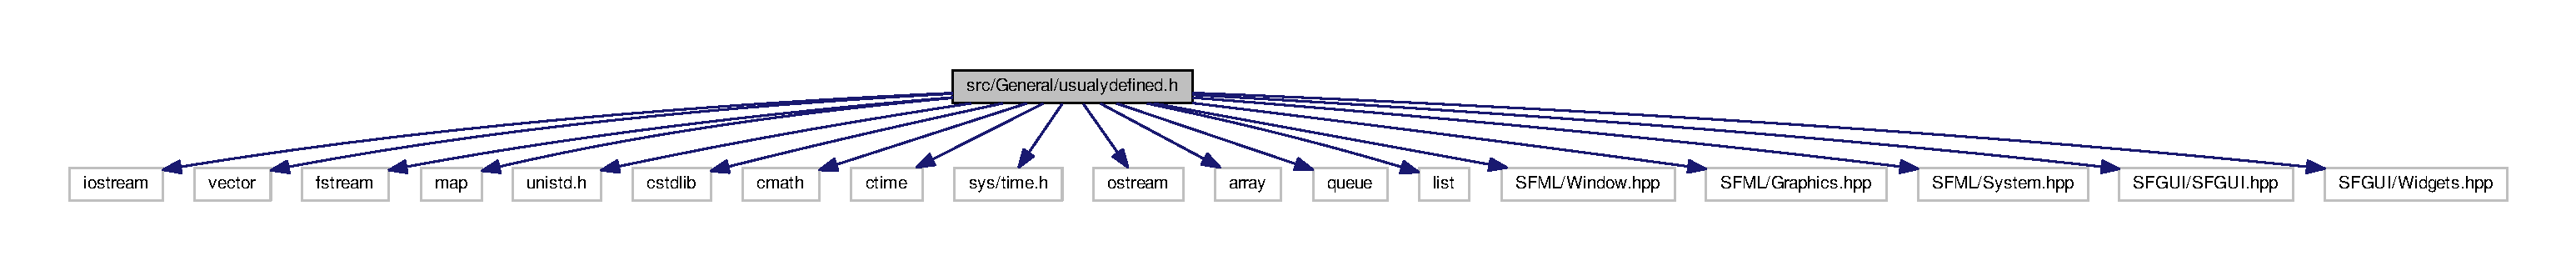
\includegraphics[width=350pt]{usualydefined_8h__incl}
\end{center}
\end{figure}
This graph shows which files directly or indirectly include this file\-:\nopagebreak
\begin{figure}[H]
\begin{center}
\leavevmode
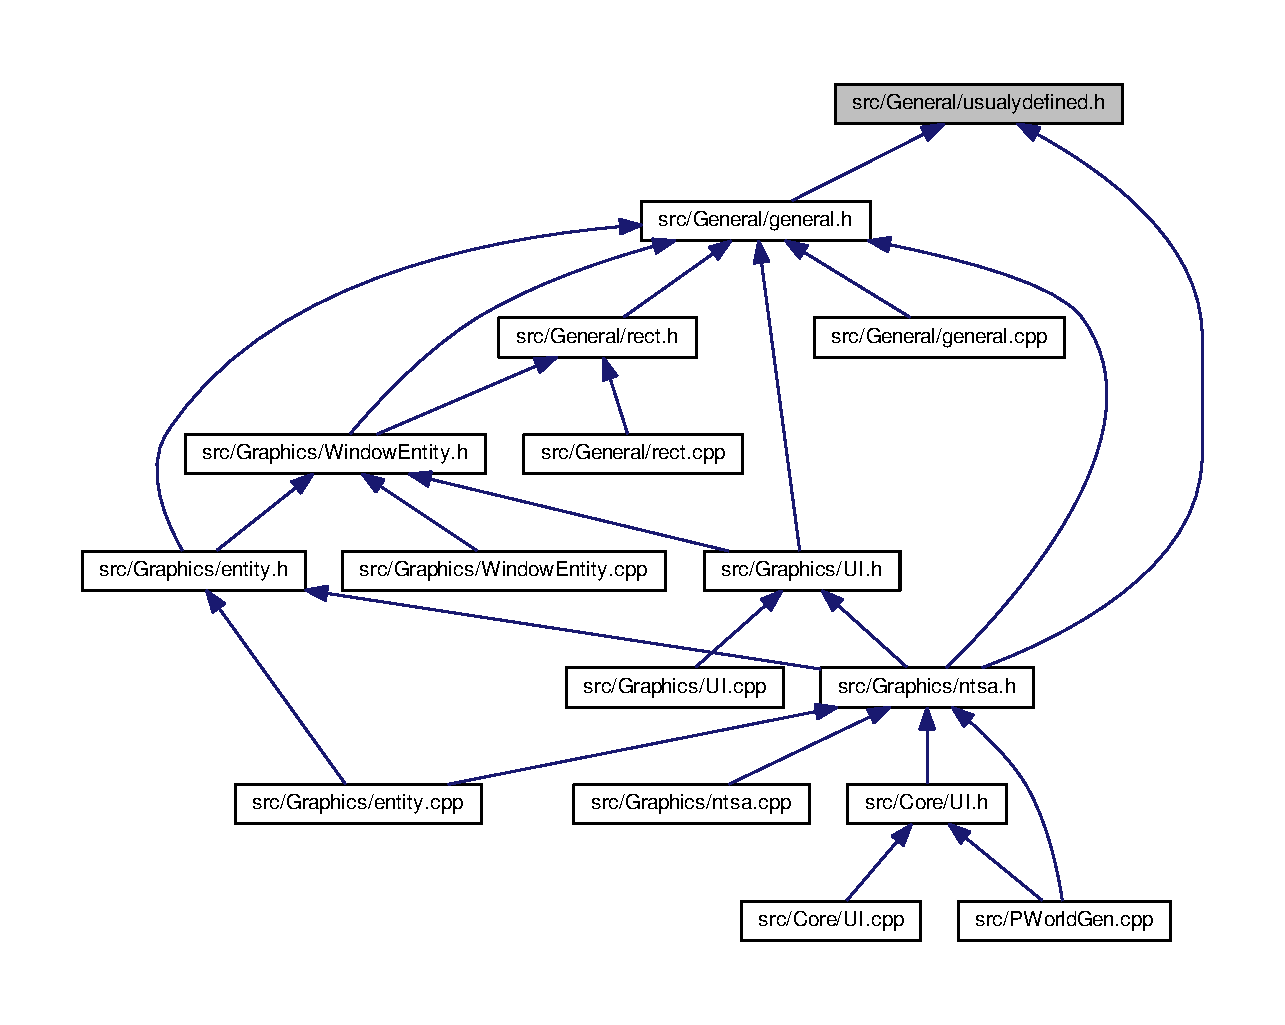
\includegraphics[width=350pt]{usualydefined_8h__dep__incl}
\end{center}
\end{figure}
\subsection*{Typedefs}
\begin{DoxyCompactItemize}
\item 
typedef unsigned char \hyperlink{usualydefined_8h_a177317577dc144582370c8b7b8efc15d}{oct\-\_\-e}
\end{DoxyCompactItemize}


\subsection{Typedef Documentation}
\hypertarget{usualydefined_8h_a177317577dc144582370c8b7b8efc15d}{\index{usualydefined.\-h@{usualydefined.\-h}!oct\-\_\-e@{oct\-\_\-e}}
\index{oct\-\_\-e@{oct\-\_\-e}!usualydefined.h@{usualydefined.\-h}}
\subsubsection[{oct\-\_\-e}]{\setlength{\rightskip}{0pt plus 5cm}typedef unsigned char {\bf oct\-\_\-e}}}\label{usualydefined_8h_a177317577dc144582370c8b7b8efc15d}


Definition at line 29 of file usualydefined.\-h.


\hypertarget{utilities_8cpp}{\section{src/\-General/utilities.cpp File Reference}
\label{utilities_8cpp}\index{src/\-General/utilities.\-cpp@{src/\-General/utilities.\-cpp}}
}
{\ttfamily \#include \char`\"{}utilities.\-h\char`\"{}}\\*
{\ttfamily \#include $<$math.\-h$>$}\\*
{\ttfamily \#include $<$cstdlib$>$}\\*
Include dependency graph for utilities.\-cpp\-:\nopagebreak
\begin{figure}[H]
\begin{center}
\leavevmode
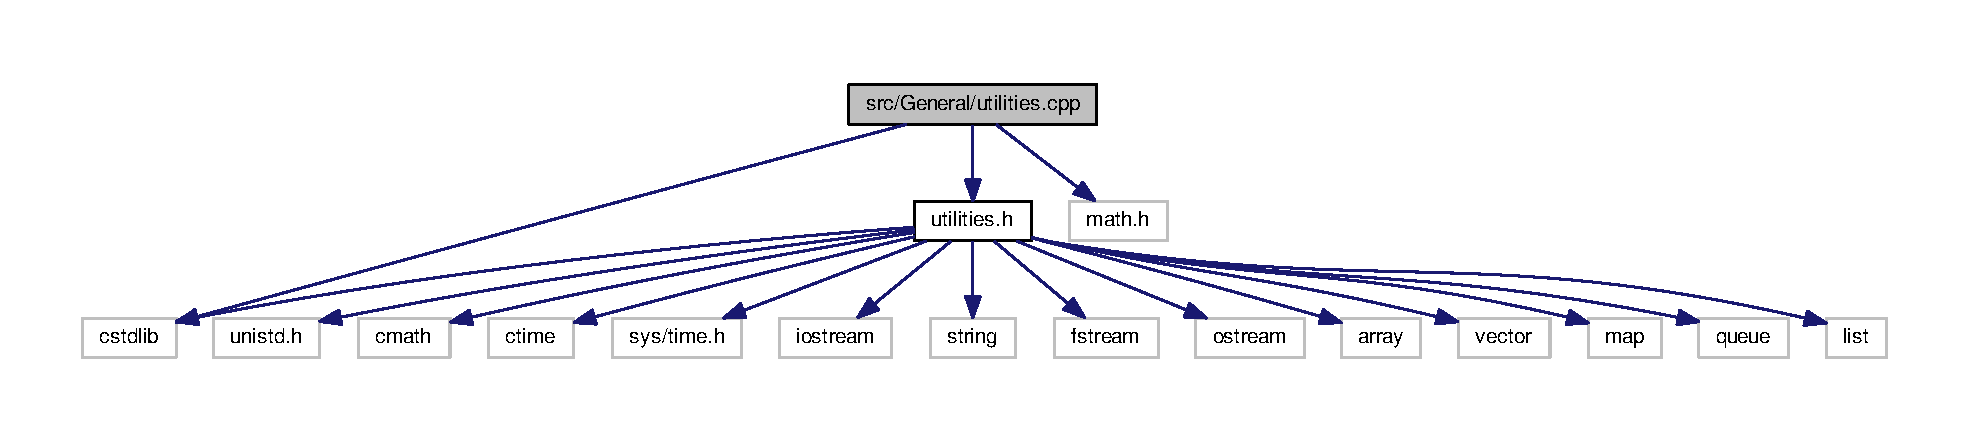
\includegraphics[width=350pt]{utilities_8cpp__incl}
\end{center}
\end{figure}
\subsection*{Data Structures}
\begin{DoxyCompactItemize}
\item 
struct \hyperlink{struct_unoise_1_1point2_dui}{Unoise\-::point2\-Dui}
\end{DoxyCompactItemize}
\subsection*{Namespaces}
\begin{DoxyCompactItemize}
\item 
\hyperlink{namespace_uchronia}{Uchronia}
\item 
\hyperlink{namespace_unoise}{Unoise}
\begin{DoxyCompactList}\small\item\em \hyperlink{namespace_uchronia}{Uchronia} noise namespace. \end{DoxyCompactList}\end{DoxyCompactItemize}
\subsection*{Macros}
\begin{DoxyCompactItemize}
\item 
\#define \hyperlink{utilities_8cpp_ac2ee50f53dbe7afff4f9e7fd890d6ac6}{nbr\-Pts\-Cote\-Paire}~(nbre\-Points\-Cote-\/1)
\end{DoxyCompactItemize}
\subsection*{Functions}
\begin{DoxyCompactItemize}
\item 
std\-::map$<$ void $\ast$, int $>$ $\ast$ \hyperlink{utilities_8cpp_a75bbbedc6b11a69f16afa80db80e0876}{get\-Cpt\-Class} (std\-::string \&nom)
\item 
void \hyperlink{utilities_8cpp_a26d990e477056c4bd6a17a77a2db2927}{aff\-Ptr\-Flag} ()
\item 
bool \hyperlink{utilities_8cpp_a06369ea5ee0568ca16b620f8faa80685}{probability} (int prob, int sur)
\begin{DoxyCompactList}\small\item\em Permet de tester une certaine probabilité \end{DoxyCompactList}\item 
string \hyperlink{utilities_8cpp_a366a670171ff9c2a7ee2a5eb953c83e3}{get\-Word} (\hyperlink{utilities_8h_ab95f123a6c9bcfee6a343170ef8c5f69}{ushort} word\-\_\-num, string \&chaine)
\item 
bool \hyperlink{utilities_8cpp_af701e0ba40a65bfd641a06968095fa75}{is\-In\-Word} (std\-::string word, std\-::string sub\-Word)
\item 
std\-::vector$<$ std\-::string $>$ \hyperlink{utilities_8cpp_a458702e54574d8cd6c8b21a11b5122c5}{get\-File\-With\-Sthx} (std\-::ifstream \&flux, unsigned int nbre\-Mots\-Attendus)
\item 
float \hyperlink{utilities_8cpp_a21d81ae15fd90d0f392e4104be872296}{positif} (int a)
\begin{DoxyCompactList}\small\item\em Renvoie le nombre en positif. \end{DoxyCompactList}\item 
void \hyperlink{namespace_unoise_a5dbbb2ae6c75efd29abd5663db08ec0e}{Unoise\-::set\-Seed} (int graine)
\item 
void \hyperlink{namespace_unoise_aa8daebdaad2fc5a125cd7b1acc7a38b4}{Unoise\-::set\-Perm\-Table} (Perm\-Table $\ast$perm)
\begin{DoxyCompactList}\small\item\em Pas obligatoire, cette fonction permet de changer lambda\-Perm\-Table. \end{DoxyCompactList}\item 
void \hyperlink{namespace_unoise_a5a1dbb7caee818c615fdfedc2ff19730}{Unoise\-::gen\-Perm\-Table} (Perm\-Table $\ast$, int)
\begin{DoxyCompactList}\small\item\em On génère la table de permutation à partir d'un seed. \end{DoxyCompactList}\item 
std\-::vector$<$ float $>$ \hyperlink{namespace_unoise_aa685d2a385bbfe1a71a1650004238202}{Unoise\-::get\-Positions\-Around} (Chunk\-Points $\ast$tableau, point2\-Dui point, int pas, std\-::array$<$ std\-::vector$<$ float $>$, 4 $>$ $\ast$points\-Environnants=nullptr, bool phase=1)
\item 
Chunk\-Points \hyperlink{namespace_unoise_accabbc2fce05f7a55bd10ec573925275}{Unoise\-::diamond\-Square\-Noise} (float x, float y, int amplitude, float res, unsigned short sub\-Divisions, int nseed=-\/1, std\-::array$<$ float, 4 $>$ $\ast$points\-Principaux=nullptr, std\-::array$<$ std\-::vector$<$ float $>$, 4 $>$ $\ast$points\-Environnants=nullptr)
\begin{DoxyCompactList}\small\item\em Midpoint displacement noise, ou Diamond square noise (nom latin\-: carrus diamus) \end{DoxyCompactList}\item 
float \hyperlink{namespace_unoise_a77b87fa88183eb7081d3ea602989c59e}{Unoise\-::perlin\-Noise} (float x, float z, float res, Perm\-Table $\ast$perm=nullptr)
\begin{DoxyCompactList}\small\item\em Fonction du bruit de perlin (float x, float z, float resolution, table de permutation)\-: \end{DoxyCompactList}\end{DoxyCompactItemize}
\subsection*{Variables}
\begin{DoxyCompactItemize}
\item 
\hyperlink{utilities_8h_aebdb70b1a700d2545ec64bc1f8319326}{Compteur\-Classe\-Type} \hyperlink{utilities_8cpp_a08697cc3a053526e6768c45bbf3f2b68}{compteur\-Classes}
\item 
Perm\-Table $\ast$ \hyperlink{namespace_unoise_acf4515c07424188371eeb9cf77d34fb3}{Unoise\-::lambda\-Perm\-Table} =nullptr
\item 
int \hyperlink{namespace_unoise_ae6356ffd0fec247f6d19c762e1757fc3}{Unoise\-::seed} =42
\end{DoxyCompactItemize}


\subsection{Macro Definition Documentation}
\hypertarget{utilities_8cpp_ac2ee50f53dbe7afff4f9e7fd890d6ac6}{\index{utilities.\-cpp@{utilities.\-cpp}!nbr\-Pts\-Cote\-Paire@{nbr\-Pts\-Cote\-Paire}}
\index{nbr\-Pts\-Cote\-Paire@{nbr\-Pts\-Cote\-Paire}!utilities.cpp@{utilities.\-cpp}}
\subsubsection[{nbr\-Pts\-Cote\-Paire}]{\setlength{\rightskip}{0pt plus 5cm}\#define nbr\-Pts\-Cote\-Paire~(nbre\-Points\-Cote-\/1)}}\label{utilities_8cpp_ac2ee50f53dbe7afff4f9e7fd890d6ac6}


Referenced by Unoise\-::diamond\-Square\-Noise().



\subsection{Function Documentation}
\hypertarget{utilities_8cpp_a26d990e477056c4bd6a17a77a2db2927}{\index{utilities.\-cpp@{utilities.\-cpp}!aff\-Ptr\-Flag@{aff\-Ptr\-Flag}}
\index{aff\-Ptr\-Flag@{aff\-Ptr\-Flag}!utilities.cpp@{utilities.\-cpp}}
\subsubsection[{aff\-Ptr\-Flag}]{\setlength{\rightskip}{0pt plus 5cm}void aff\-Ptr\-Flag (
\begin{DoxyParamCaption}
{}
\end{DoxyParamCaption}
)}}\label{utilities_8cpp_a26d990e477056c4bd6a17a77a2db2927}


Definition at line 13 of file utilities.\-cpp.

\hypertarget{utilities_8cpp_a75bbbedc6b11a69f16afa80db80e0876}{\index{utilities.\-cpp@{utilities.\-cpp}!get\-Cpt\-Class@{get\-Cpt\-Class}}
\index{get\-Cpt\-Class@{get\-Cpt\-Class}!utilities.cpp@{utilities.\-cpp}}
\subsubsection[{get\-Cpt\-Class}]{\setlength{\rightskip}{0pt plus 5cm}std\-::map$<$void $\ast$, int$>$$\ast$ get\-Cpt\-Class (
\begin{DoxyParamCaption}
\item[{std\-::string \&}]{nom}
\end{DoxyParamCaption}
)}}\label{utilities_8cpp_a75bbbedc6b11a69f16afa80db80e0876}


Definition at line 8 of file utilities.\-cpp.

\hypertarget{utilities_8cpp_a458702e54574d8cd6c8b21a11b5122c5}{\index{utilities.\-cpp@{utilities.\-cpp}!get\-File\-With\-Sthx@{get\-File\-With\-Sthx}}
\index{get\-File\-With\-Sthx@{get\-File\-With\-Sthx}!utilities.cpp@{utilities.\-cpp}}
\subsubsection[{get\-File\-With\-Sthx}]{\setlength{\rightskip}{0pt plus 5cm}std\-::vector$<$std\-::string$>$ get\-File\-With\-Sthx (
\begin{DoxyParamCaption}
\item[{std\-::ifstream \&}]{flux, }
\item[{unsigned int}]{nbre\-Mots\-Attendus = {\ttfamily {\bf I\-N\-T\-\_\-\-I\-M\-P\-R\-O\-B\-A\-B\-L\-E}}}
\end{DoxyParamCaption}
)}}\label{utilities_8cpp_a458702e54574d8cd6c8b21a11b5122c5}
Lis dans le fichier donné une liste de mots suivant ces conditions\-: si le premier mot de la chaîne \par
se termine par \char`\"{}\-:\char`\"{}, on l'ignore (il est alors considéré comme une sorte de commentaire) et si le mot \par
est \char`\"{};\char`\"{}, on s'arrête de rajouter des mots dans le vector. Enfin, on ne retourne qu'une nombre de mots égale\par
à {\itshape nbre\-Mots\-Attendus}. 

Definition at line 77 of file utilities.\-cpp.



Here is the call graph for this function\-:\nopagebreak
\begin{figure}[H]
\begin{center}
\leavevmode
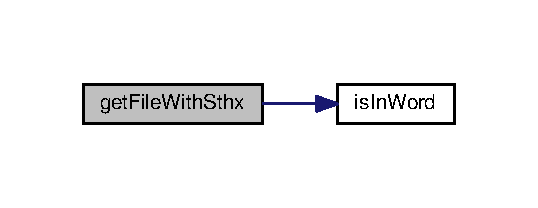
\includegraphics[width=258pt]{utilities_8cpp_a458702e54574d8cd6c8b21a11b5122c5_cgraph}
\end{center}
\end{figure}


\hypertarget{utilities_8cpp_a366a670171ff9c2a7ee2a5eb953c83e3}{\index{utilities.\-cpp@{utilities.\-cpp}!get\-Word@{get\-Word}}
\index{get\-Word@{get\-Word}!utilities.cpp@{utilities.\-cpp}}
\subsubsection[{get\-Word}]{\setlength{\rightskip}{0pt plus 5cm}string get\-Word (
\begin{DoxyParamCaption}
\item[{{\bf ushort}}]{word\-\_\-num, }
\item[{string \&}]{chaine}
\end{DoxyParamCaption}
)}}\label{utilities_8cpp_a366a670171ff9c2a7ee2a5eb953c83e3}


Definition at line 40 of file utilities.\-cpp.



Referenced by Window\-Entity\-::load\-From\-Instructions().

\hypertarget{utilities_8cpp_af701e0ba40a65bfd641a06968095fa75}{\index{utilities.\-cpp@{utilities.\-cpp}!is\-In\-Word@{is\-In\-Word}}
\index{is\-In\-Word@{is\-In\-Word}!utilities.cpp@{utilities.\-cpp}}
\subsubsection[{is\-In\-Word}]{\setlength{\rightskip}{0pt plus 5cm}bool is\-In\-Word (
\begin{DoxyParamCaption}
\item[{std\-::string}]{word, }
\item[{std\-::string}]{sub\-Word}
\end{DoxyParamCaption}
)}}\label{utilities_8cpp_af701e0ba40a65bfd641a06968095fa75}
\begin{DoxyReturn}{Returns}
true si {\itshape sub\-Word} est dans {\itshape word} 
\end{DoxyReturn}


Definition at line 59 of file utilities.\-cpp.



Referenced by get\-File\-With\-Sthx().

\hypertarget{utilities_8cpp_a21d81ae15fd90d0f392e4104be872296}{\index{utilities.\-cpp@{utilities.\-cpp}!positif@{positif}}
\index{positif@{positif}!utilities.cpp@{utilities.\-cpp}}
\subsubsection[{positif}]{\setlength{\rightskip}{0pt plus 5cm}float positif (
\begin{DoxyParamCaption}
\item[{int}]{a}
\end{DoxyParamCaption}
)}}\label{utilities_8cpp_a21d81ae15fd90d0f392e4104be872296}


Renvoie le nombre en positif. 



Definition at line 105 of file utilities.\-cpp.

\hypertarget{utilities_8cpp_a06369ea5ee0568ca16b620f8faa80685}{\index{utilities.\-cpp@{utilities.\-cpp}!probability@{probability}}
\index{probability@{probability}!utilities.cpp@{utilities.\-cpp}}
\subsubsection[{probability}]{\setlength{\rightskip}{0pt plus 5cm}bool probability (
\begin{DoxyParamCaption}
\item[{int}]{prob, }
\item[{int}]{sur}
\end{DoxyParamCaption}
)}}\label{utilities_8cpp_a06369ea5ee0568ca16b620f8faa80685}


Permet de tester une certaine probabilité 



Definition at line 35 of file utilities.\-cpp.



\subsection{Variable Documentation}
\hypertarget{utilities_8cpp_a08697cc3a053526e6768c45bbf3f2b68}{\index{utilities.\-cpp@{utilities.\-cpp}!compteur\-Classes@{compteur\-Classes}}
\index{compteur\-Classes@{compteur\-Classes}!utilities.cpp@{utilities.\-cpp}}
\subsubsection[{compteur\-Classes}]{\setlength{\rightskip}{0pt plus 5cm}{\bf Compteur\-Classe\-Type} compteur\-Classes}}\label{utilities_8cpp_a08697cc3a053526e6768c45bbf3f2b68}


Definition at line 7 of file utilities.\-cpp.



Referenced by aff\-Ptr\-Flag(), and get\-Cpt\-Class().


\hypertarget{utilities_8h}{\section{src/\-General/utilities.h File Reference}
\label{utilities_8h}\index{src/\-General/utilities.\-h@{src/\-General/utilities.\-h}}
}
{\ttfamily \#include $<$unistd.\-h$>$}\\*
{\ttfamily \#include $<$cstdlib$>$}\\*
{\ttfamily \#include $<$cmath$>$}\\*
{\ttfamily \#include $<$ctime$>$}\\*
{\ttfamily \#include $<$sys/time.\-h$>$}\\*
{\ttfamily \#include $<$iostream$>$}\\*
{\ttfamily \#include $<$string$>$}\\*
{\ttfamily \#include $<$fstream$>$}\\*
{\ttfamily \#include $<$ostream$>$}\\*
{\ttfamily \#include $<$array$>$}\\*
{\ttfamily \#include $<$vector$>$}\\*
{\ttfamily \#include $<$map$>$}\\*
{\ttfamily \#include $<$queue$>$}\\*
{\ttfamily \#include $<$list$>$}\\*
Include dependency graph for utilities.\-h\-:\nopagebreak
\begin{figure}[H]
\begin{center}
\leavevmode
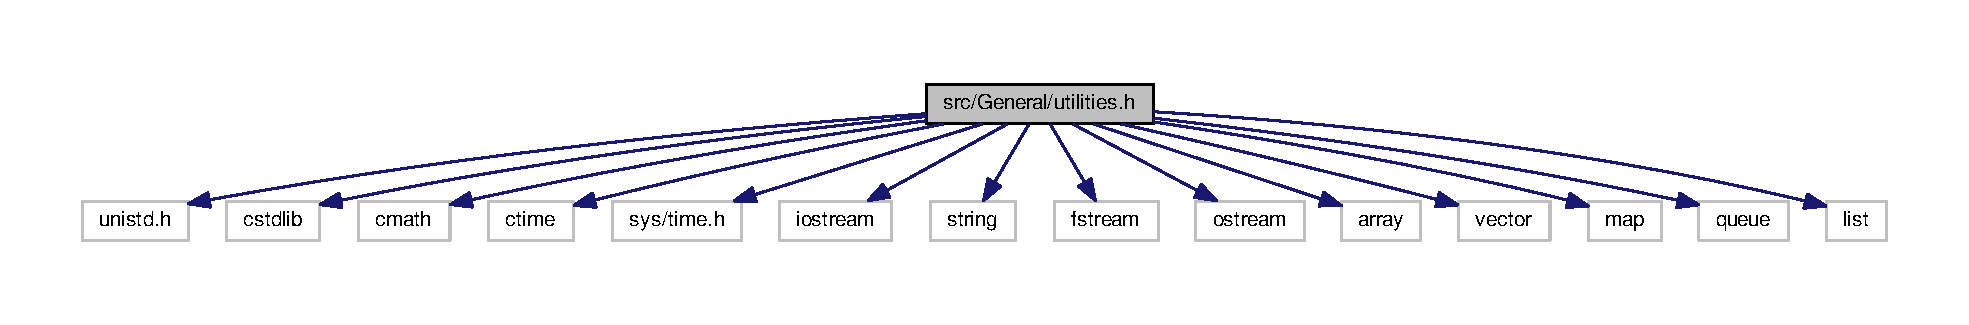
\includegraphics[width=350pt]{utilities_8h__incl}
\end{center}
\end{figure}
This graph shows which files directly or indirectly include this file\-:
\nopagebreak
\begin{figure}[H]
\begin{center}
\leavevmode
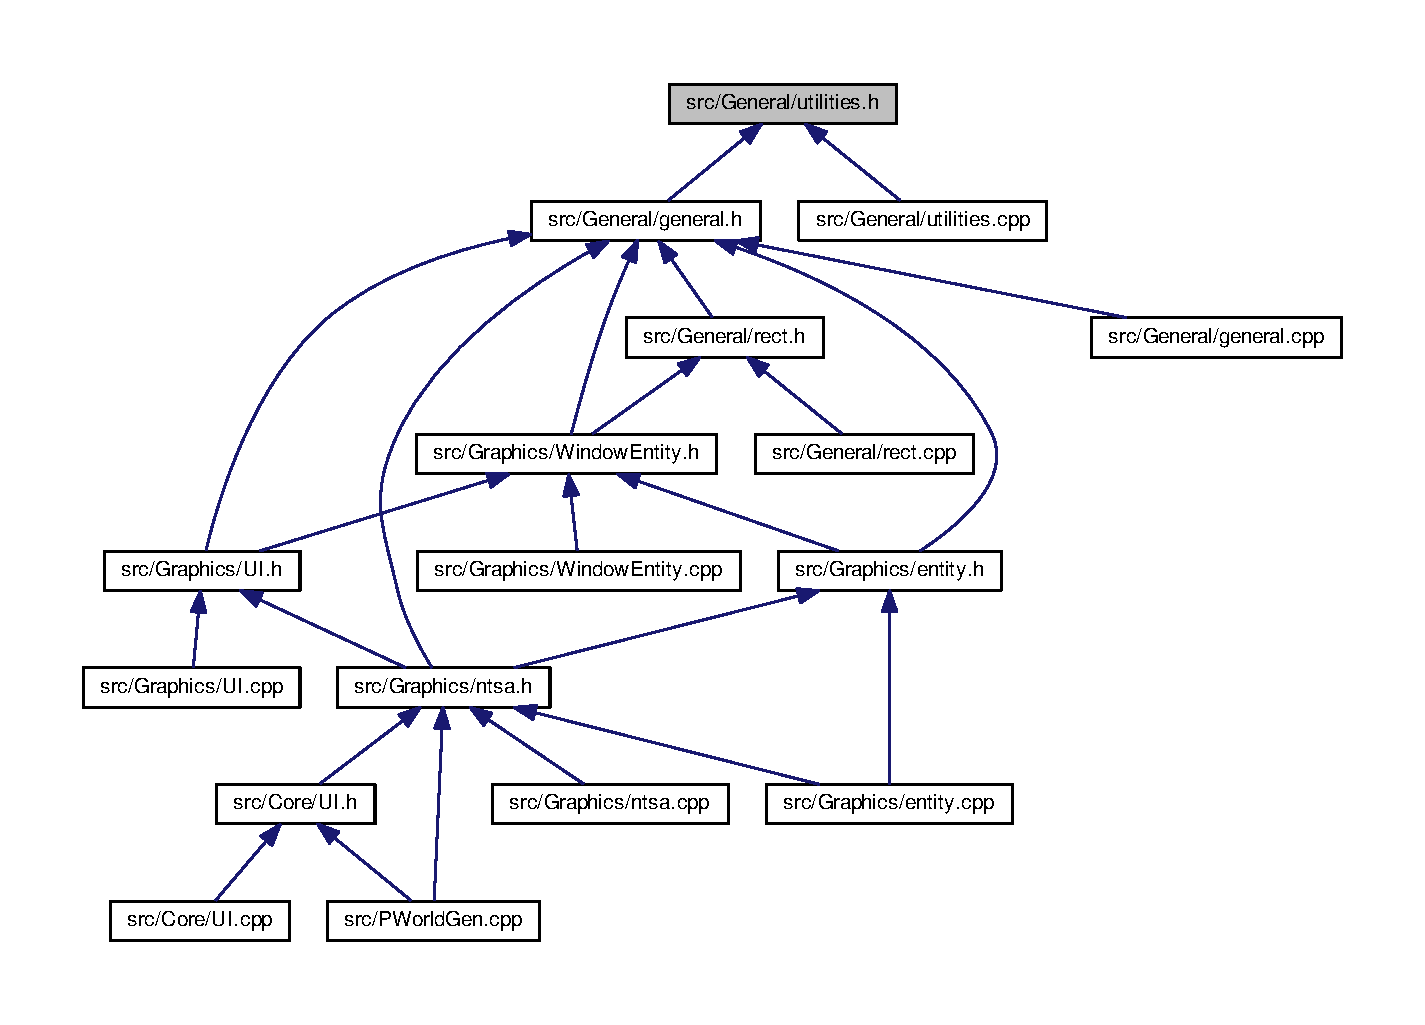
\includegraphics[width=350pt]{utilities_8h__dep__incl}
\end{center}
\end{figure}
\subsection*{Data Structures}
\begin{DoxyCompactItemize}
\item 
struct \hyperlink{struct_unoise_1_1_diamond_perm_table}{Unoise\-::\-Diamond\-Perm\-Table}
\begin{DoxyCompactList}\small\item\em Stock a Perm\-Table \char`\"{}\-Diamond\char`\"{}. \end{DoxyCompactList}\end{DoxyCompactItemize}
\subsection*{Namespaces}
\begin{DoxyCompactItemize}
\item 
\hyperlink{namespace_unoise}{Unoise}
\begin{DoxyCompactList}\small\item\em \hyperlink{namespace_uchronia}{Uchronia} noise namespace. \end{DoxyCompactList}\end{DoxyCompactItemize}
\subsection*{Macros}
\begin{DoxyCompactItemize}
\item 
\#define \hyperlink{utilities_8h_aef26ade3602d14eb964ae87184aae00e}{D\-E\-B\-U\-G\-M\-O\-D}
\item 
\#define \hyperlink{utilities_8h_a13cd3c33b3603e0b57d2d0744c411de3}{P\-R\-\_\-\-W\-H\-I\-T\-E}~30
\item 
\#define \hyperlink{utilities_8h_a84132e35e6574c53f808afdfd2f912c4}{P\-R\-\_\-\-R\-E\-D}~31
\item 
\#define \hyperlink{utilities_8h_a6e22edb41217878a4071d0d4fca44797}{P\-R\-\_\-\-G\-R\-E\-E\-N}~32
\item 
\#define \hyperlink{utilities_8h_a3f6d6e64b5bc3e9fe0700f0f01410d74}{P\-R\-\_\-\-Y\-E\-L\-L\-O\-W}~33
\item 
\#define \hyperlink{utilities_8h_a0382d53ae1847bfe75dfca06abb1a429}{P\-R\-\_\-\-B\-L\-U\-E}~34
\item 
\#define \hyperlink{utilities_8h_aa7280378cd45386f5e22c2bb93bb064c}{P\-R\-\_\-\-P\-U\-R\-P\-L\-E}~35
\item 
\#define \hyperlink{utilities_8h_a52efd9c68a31467dc1264602589ab057}{P\-R\-\_\-\-L\-I\-G\-H\-T\-B\-L\-U\-E}~36
\item 
\#define \hyperlink{utilities_8h_a1266b9f426819dd36243651569f96d09}{P\-R\-\_\-\-G\-R\-E\-Y}~37
\item 
\#define \hyperlink{utilities_8h_a4531ebacd4bb0fbc8872c3fd30dd7edd}{C\-O\-L\-O\-R\-E\-D\-\_\-\-P\-R\-I\-N\-T}(param1, param)~std\-::cout$<$$<$\char`\"{}\textbackslash{}033\mbox{[}\char`\"{}$<$$<$param$<$$<$\char`\"{}m\char`\"{}$<$$<$param1$<$$<$\char`\"{}\textbackslash{}033\mbox{[}30m\char`\"{}$<$$<$std\-::endl
\item 
\#define \hyperlink{utilities_8h_a68a06cdb6de2f5020a7def6942eaccad}{P\-I\-M\-P}(txt)~\hyperlink{utilities_8h_a4531ebacd4bb0fbc8872c3fd30dd7edd}{C\-O\-L\-O\-R\-E\-D\-\_\-\-P\-R\-I\-N\-T}(\char`\"{}/!\textbackslash{}\textbackslash{}P\-I\-M\-P S\-P\-O\-T\-T\-E\-D/!\textbackslash{}\textbackslash{}\-: \char`\"{}$<$$<$txt, \hyperlink{utilities_8h_a52efd9c68a31467dc1264602589ab057}{P\-R\-\_\-\-L\-I\-G\-H\-T\-B\-L\-U\-E})
\item 
\#define \hyperlink{utilities_8h_a2308dd37abb259babc5baf6805bce76f}{D\-E\-B\-U\-G}(txt)~\hyperlink{utilities_8h_a4531ebacd4bb0fbc8872c3fd30dd7edd}{C\-O\-L\-O\-R\-E\-D\-\_\-\-P\-R\-I\-N\-T}(\char`\"{}D\-E\-B\-U\-G\-: \char`\"{}$<$$<$txt, \hyperlink{utilities_8h_a0382d53ae1847bfe75dfca06abb1a429}{P\-R\-\_\-\-B\-L\-U\-E})
\item 
\#define \hyperlink{utilities_8h_aec7008c0513b376e00b01637193ff746}{I\-N\-F\-O}(txt)~\hyperlink{utilities_8h_a4531ebacd4bb0fbc8872c3fd30dd7edd}{C\-O\-L\-O\-R\-E\-D\-\_\-\-P\-R\-I\-N\-T}(\char`\"{}I\-N\-F\-O\-: \char`\"{}$<$$<$txt, \hyperlink{utilities_8h_a1266b9f426819dd36243651569f96d09}{P\-R\-\_\-\-G\-R\-E\-Y})
\item 
\#define \hyperlink{utilities_8h_aeb7de637805f40ca1d6f9dd57423c922}{W\-A\-R\-N\-I\-N\-G}(txt)~\hyperlink{utilities_8h_a4531ebacd4bb0fbc8872c3fd30dd7edd}{C\-O\-L\-O\-R\-E\-D\-\_\-\-P\-R\-I\-N\-T}(\char`\"{}W\-A\-R\-N\-I\-N\-G\-: \char`\"{}$<$$<$txt, \hyperlink{utilities_8h_a3f6d6e64b5bc3e9fe0700f0f01410d74}{P\-R\-\_\-\-Y\-E\-L\-L\-O\-W})
\item 
\#define \hyperlink{utilities_8h_acae6718a3f55bf5d018a4b458d5492c0}{E\-R\-R\-O\-R}(txt)~\hyperlink{utilities_8h_a4531ebacd4bb0fbc8872c3fd30dd7edd}{C\-O\-L\-O\-R\-E\-D\-\_\-\-P\-R\-I\-N\-T}(\char`\"{}E\-R\-R\-O\-R\-: \char`\"{}$<$$<$txt, \hyperlink{utilities_8h_a84132e35e6574c53f808afdfd2f912c4}{P\-R\-\_\-\-R\-E\-D})
\item 
\#define \hyperlink{utilities_8h_aac9431e400a41b9c4d231c83e74c7729}{C\-R\-I\-T\-I\-C\-\_\-\-E\-R\-R\-O\-R}(txt)~\hyperlink{utilities_8h_a4531ebacd4bb0fbc8872c3fd30dd7edd}{C\-O\-L\-O\-R\-E\-D\-\_\-\-P\-R\-I\-N\-T}(\char`\"{}/!\textbackslash{}\textbackslash{}C\-R\-I\-T\-I\-C \hyperlink{utilities_8h_acae6718a3f55bf5d018a4b458d5492c0}{E\-R\-R\-O\-R}/!\textbackslash{}\textbackslash{}\-: \char`\"{}$<$$<$txt, \hyperlink{utilities_8h_aa7280378cd45386f5e22c2bb93bb064c}{P\-R\-\_\-\-P\-U\-R\-P\-L\-E});std\-::cout$<$$<$1/0$<$$<$std\-::endl
\item 
\#define \hyperlink{utilities_8h_a33b8df933d992ff1be22c0d05191c79e}{aff\-In\-Debug}(message, entree)~entree(message)
\item 
\#define \hyperlink{utilities_8h_a0d7644a795aa2dd33f01ef184f3f672a}{R\-A\-N\-D}(min, max)~( (rand() \% (max-\/min+1))+min )
\item 
\#define \hyperlink{utilities_8h_a6042b13d082c692eb725acf5dea13b7b}{M\-S\-L\-E\-E\-P}(msecs)~usleep(msecs$\ast$1000)
\item 
\#define \hyperlink{utilities_8h_a7e9d6bf9d4bba615fca7196a16b33b4e}{C\-A\-R\-R\-E}(var)~(var$\ast$var)
\item 
\#define \hyperlink{utilities_8h_a6e2f5e51b142e0be9a976a8bdda7bd9d}{I\-S\-I\-N\-T\-E\-G\-R\-E\-R}(result)~(result==(int)result)
\item 
\#define \hyperlink{utilities_8h_ae92c1b3f2d775c70c1ce3f3e8c0a9550}{I\-S\-P\-O\-S\-I\-T\-I\-V\-E}(number)~(number$>$=0)
\item 
\#define \hyperlink{utilities_8h_a19d3faf4a80fd3b884fb877f87663ef1}{cut\-Diz}(nombre\-\_\-, nb\-Integrers\-\_\-)~(nombre\-\_\-/(10$\ast$(long)((nombre\-\_\-/10)$\ast$pow(10, nb\-Integrers\-\_\-)))
\begin{DoxyCompactList}\small\item\em Cette fonction ne garde qu'un certain nombre de chiffres de la partie entière. \end{DoxyCompactList}\item 
\#define \hyperlink{utilities_8h_aa536229c7484bedc4cb489147f5522de}{D\-I\-V\-I\-S\-I\-B\-L\-E\-\_\-\-P\-A\-R}(nbre, diviseur)~(nbre/((float)diviseur)==(short)nbre/diviseur)
\item 
\#define \hyperlink{utilities_8h_a5c7ba19c1dea5792082649d98514e3cd}{I\-N\-T\-\_\-\-I\-M\-P\-R\-O\-B\-A\-B\-L\-E}~4294967295
\item 
\#define \hyperlink{utilities_8h_a7a89272eb35d77be1b8a785b12febb6d}{ptr\-Flag\-Inc}(nomclasse, ptr\-Classe)~\hyperlink{utilities_8cpp_a08697cc3a053526e6768c45bbf3f2b68}{compteur\-Classes}\mbox{[}nomclasse\mbox{]}.at(ptr\-Classe) += 1
\item 
\#define \hyperlink{utilities_8h_a752fdc9393564b629934730e70f77c1f}{ptr\-Flag\-Dec}(nomclasse, ptr\-Classe)~\hyperlink{utilities_8cpp_a08697cc3a053526e6768c45bbf3f2b68}{compteur\-Classes}\mbox{[}nomclasse\mbox{]}.at(ptr\-Classe) -\/= 1
\end{DoxyCompactItemize}
\subsection*{Typedefs}
\begin{DoxyCompactItemize}
\item 
typedef std\-::map$<$ std\-::string, \\*
std\-::map$<$ void $\ast$, int $>$ $>$ \hyperlink{utilities_8h_aebdb70b1a700d2545ec64bc1f8319326}{Compteur\-Classe\-Type}
\item 
typedef unsigned char \hyperlink{utilities_8h_a177317577dc144582370c8b7b8efc15d}{oct\-\_\-e}
\item 
typedef unsigned char \hyperlink{utilities_8h_a65f85814a8290f9797005d3b28e7e5fc}{uchar}
\item 
typedef unsigned short \hyperlink{utilities_8h_ab95f123a6c9bcfee6a343170ef8c5f69}{ushort}
\item 
typedef std\-::array$<$ unsigned \\*
short, 256 $>$ \hyperlink{namespace_unoise_ae11142038f2dd1bea2711b2b99bbfaf6}{Unoise\-::\-Perm\-Table}
\item 
typedef std\-::vector\\*
$<$ std\-::vector$<$ float $>$ $>$ \hyperlink{namespace_unoise_ac1e5c6227ab68e4e8c1ad57fdbddf51b}{Unoise\-::\-Chunk\-Points}
\end{DoxyCompactItemize}
\subsection*{Functions}
\begin{DoxyCompactItemize}
\item 
std\-::map$<$ void $\ast$, int $>$ $\ast$ \hyperlink{utilities_8h_a75bbbedc6b11a69f16afa80db80e0876}{get\-Cpt\-Class} (std\-::string \&nom)
\item 
void \hyperlink{utilities_8h_a26d990e477056c4bd6a17a77a2db2927}{aff\-Ptr\-Flag} ()
\item 
bool \hyperlink{utilities_8h_a06369ea5ee0568ca16b620f8faa80685}{probability} (int prob, int sur)
\begin{DoxyCompactList}\small\item\em Permet de tester une certaine probabilité \end{DoxyCompactList}\item 
float \hyperlink{utilities_8h_a21d81ae15fd90d0f392e4104be872296}{positif} (int a)
\begin{DoxyCompactList}\small\item\em Renvoie le nombre en positif. \end{DoxyCompactList}\item 
std\-::string \hyperlink{utilities_8h_aed89159b1527605074e6ec1ddf945e69}{get\-Word} (\hyperlink{utilities_8h_ab95f123a6c9bcfee6a343170ef8c5f69}{ushort} word\-\_\-num, std\-::string \&chaine)
\begin{DoxyCompactList}\small\item\em Donne le mot n°{\itshape word\-\_\-num} dans la chaine chaine, à noter que word\-\_\-num commence par 0;. \end{DoxyCompactList}\item 
bool \hyperlink{utilities_8h_af701e0ba40a65bfd641a06968095fa75}{is\-In\-Word} (std\-::string word, std\-::string sub\-Word)
\item 
std\-::vector$<$ std\-::string $>$ \hyperlink{utilities_8h_a952a8c5f0067bb44afe28b66fdfa555b}{get\-File\-With\-Sthx} (std\-::ifstream \&flux, unsigned int nbre\-Mots\-Attendus=\hyperlink{utilities_8h_a5c7ba19c1dea5792082649d98514e3cd}{I\-N\-T\-\_\-\-I\-M\-P\-R\-O\-B\-A\-B\-L\-E})
\item 
void \hyperlink{namespace_unoise_aa8daebdaad2fc5a125cd7b1acc7a38b4}{Unoise\-::set\-Perm\-Table} (Perm\-Table $\ast$perm)
\begin{DoxyCompactList}\small\item\em Pas obligatoire, cette fonction permet de changer lambda\-Perm\-Table. \end{DoxyCompactList}\item 
void \hyperlink{namespace_unoise_a5dbbb2ae6c75efd29abd5663db08ec0e}{Unoise\-::set\-Seed} (int graine)
\item 
void \hyperlink{namespace_unoise_a5a1dbb7caee818c615fdfedc2ff19730}{Unoise\-::gen\-Perm\-Table} (Perm\-Table $\ast$, int)
\begin{DoxyCompactList}\small\item\em On génère la table de permutation à partir d'un seed. \end{DoxyCompactList}\item 
float \hyperlink{namespace_unoise_a77b87fa88183eb7081d3ea602989c59e}{Unoise\-::perlin\-Noise} (float x, float z, float res, Perm\-Table $\ast$perm=nullptr)
\begin{DoxyCompactList}\small\item\em Fonction du bruit de perlin (float x, float z, float resolution, table de permutation)\-: \end{DoxyCompactList}\item 
Chunk\-Points \hyperlink{namespace_unoise_accabbc2fce05f7a55bd10ec573925275}{Unoise\-::diamond\-Square\-Noise} (float x, float y, int amplitude, float res, unsigned short sub\-Divisions, int nseed=-\/1, std\-::array$<$ float, 4 $>$ $\ast$points\-Principaux=nullptr, std\-::array$<$ std\-::vector$<$ float $>$, 4 $>$ $\ast$points\-Environnants=nullptr)
\begin{DoxyCompactList}\small\item\em Midpoint displacement noise, ou Diamond square noise (nom latin\-: carrus diamus) \end{DoxyCompactList}\end{DoxyCompactItemize}


\subsection{Macro Definition Documentation}
\hypertarget{utilities_8h_a33b8df933d992ff1be22c0d05191c79e}{\index{utilities.\-h@{utilities.\-h}!aff\-In\-Debug@{aff\-In\-Debug}}
\index{aff\-In\-Debug@{aff\-In\-Debug}!utilities.h@{utilities.\-h}}
\subsubsection[{aff\-In\-Debug}]{\setlength{\rightskip}{0pt plus 5cm}\#define aff\-In\-Debug(
\begin{DoxyParamCaption}
\item[{}]{message, }
\item[{}]{entree}
\end{DoxyParamCaption}
)~entree(message)}}\label{utilities_8h_a33b8df933d992ff1be22c0d05191c79e}


Definition at line 45 of file utilities.\-h.



Referenced by Window\-Entity\-::actuate\-Sprite(), Sprite\-List\-::\-Add\-Sprite(), Window\-Entity\-::add\-Texture(), Texture\-List\-::load\-Textures(), Sprite\-List\-::\-Remove\-Sprite(), and Window\-Entity\-::\-Window\-Entity().

\hypertarget{utilities_8h_a7e9d6bf9d4bba615fca7196a16b33b4e}{\index{utilities.\-h@{utilities.\-h}!C\-A\-R\-R\-E@{C\-A\-R\-R\-E}}
\index{C\-A\-R\-R\-E@{C\-A\-R\-R\-E}!utilities.h@{utilities.\-h}}
\subsubsection[{C\-A\-R\-R\-E}]{\setlength{\rightskip}{0pt plus 5cm}\#define C\-A\-R\-R\-E(
\begin{DoxyParamCaption}
\item[{}]{var}
\end{DoxyParamCaption}
)~(var$\ast$var)}}\label{utilities_8h_a7e9d6bf9d4bba615fca7196a16b33b4e}


Definition at line 56 of file utilities.\-h.



Referenced by Unoise\-::diamond\-Square\-Noise().

\hypertarget{utilities_8h_a4531ebacd4bb0fbc8872c3fd30dd7edd}{\index{utilities.\-h@{utilities.\-h}!C\-O\-L\-O\-R\-E\-D\-\_\-\-P\-R\-I\-N\-T@{C\-O\-L\-O\-R\-E\-D\-\_\-\-P\-R\-I\-N\-T}}
\index{C\-O\-L\-O\-R\-E\-D\-\_\-\-P\-R\-I\-N\-T@{C\-O\-L\-O\-R\-E\-D\-\_\-\-P\-R\-I\-N\-T}!utilities.h@{utilities.\-h}}
\subsubsection[{C\-O\-L\-O\-R\-E\-D\-\_\-\-P\-R\-I\-N\-T}]{\setlength{\rightskip}{0pt plus 5cm}\#define C\-O\-L\-O\-R\-E\-D\-\_\-\-P\-R\-I\-N\-T(
\begin{DoxyParamCaption}
\item[{}]{param1, }
\item[{}]{param}
\end{DoxyParamCaption}
)~std\-::cout$<$$<$\char`\"{}\textbackslash{}033\mbox{[}\char`\"{}$<$$<$param$<$$<$\char`\"{}m\char`\"{}$<$$<$param1$<$$<$\char`\"{}\textbackslash{}033\mbox{[}30m\char`\"{}$<$$<$std\-::endl}}\label{utilities_8h_a4531ebacd4bb0fbc8872c3fd30dd7edd}


Definition at line 35 of file utilities.\-h.

\hypertarget{utilities_8h_aac9431e400a41b9c4d231c83e74c7729}{\index{utilities.\-h@{utilities.\-h}!C\-R\-I\-T\-I\-C\-\_\-\-E\-R\-R\-O\-R@{C\-R\-I\-T\-I\-C\-\_\-\-E\-R\-R\-O\-R}}
\index{C\-R\-I\-T\-I\-C\-\_\-\-E\-R\-R\-O\-R@{C\-R\-I\-T\-I\-C\-\_\-\-E\-R\-R\-O\-R}!utilities.h@{utilities.\-h}}
\subsubsection[{C\-R\-I\-T\-I\-C\-\_\-\-E\-R\-R\-O\-R}]{\setlength{\rightskip}{0pt plus 5cm}\#define C\-R\-I\-T\-I\-C\-\_\-\-E\-R\-R\-O\-R(
\begin{DoxyParamCaption}
\item[{}]{txt}
\end{DoxyParamCaption}
)~{\bf C\-O\-L\-O\-R\-E\-D\-\_\-\-P\-R\-I\-N\-T}(\char`\"{}/!\textbackslash{}\textbackslash{}C\-R\-I\-T\-I\-C {\bf E\-R\-R\-O\-R}/!\textbackslash{}\textbackslash{}\-: \char`\"{}$<$$<$txt, {\bf P\-R\-\_\-\-P\-U\-R\-P\-L\-E});std\-::cout$<$$<$1/0$<$$<$std\-::endl}}\label{utilities_8h_aac9431e400a41b9c4d231c83e74c7729}


Definition at line 42 of file utilities.\-h.

\hypertarget{utilities_8h_a19d3faf4a80fd3b884fb877f87663ef1}{\index{utilities.\-h@{utilities.\-h}!cut\-Diz@{cut\-Diz}}
\index{cut\-Diz@{cut\-Diz}!utilities.h@{utilities.\-h}}
\subsubsection[{cut\-Diz}]{\setlength{\rightskip}{0pt plus 5cm}\#define cut\-Diz(
\begin{DoxyParamCaption}
\item[{}]{nombre\-\_\-, }
\item[{}]{nb\-Integrers\-\_\-}
\end{DoxyParamCaption}
)~(nombre\-\_\-/(10$\ast$(long)((nombre\-\_\-/10)$\ast$pow(10, nb\-Integrers\-\_\-)))}}\label{utilities_8h_a19d3faf4a80fd3b884fb877f87663ef1}


Cette fonction ne garde qu'un certain nombre de chiffres de la partie entière. 



Definition at line 64 of file utilities.\-h.

\hypertarget{utilities_8h_a2308dd37abb259babc5baf6805bce76f}{\index{utilities.\-h@{utilities.\-h}!D\-E\-B\-U\-G@{D\-E\-B\-U\-G}}
\index{D\-E\-B\-U\-G@{D\-E\-B\-U\-G}!utilities.h@{utilities.\-h}}
\subsubsection[{D\-E\-B\-U\-G}]{\setlength{\rightskip}{0pt plus 5cm}\#define D\-E\-B\-U\-G(
\begin{DoxyParamCaption}
\item[{}]{txt}
\end{DoxyParamCaption}
)~{\bf C\-O\-L\-O\-R\-E\-D\-\_\-\-P\-R\-I\-N\-T}(\char`\"{}D\-E\-B\-U\-G\-: \char`\"{}$<$$<$txt, {\bf P\-R\-\_\-\-B\-L\-U\-E})}}\label{utilities_8h_a2308dd37abb259babc5baf6805bce76f}


Definition at line 38 of file utilities.\-h.



Referenced by Window\-Entity\-::actuate\-Sprite(), Sprite\-List\-::\-Add\-Sprite(), aff\-Ptr\-Flag(), Texture\-List\-::load\-Textures(), Sprite\-List\-::\-Remove\-Sprite(), and Window\-Entity\-::\-Window\-Entity().

\hypertarget{utilities_8h_aef26ade3602d14eb964ae87184aae00e}{\index{utilities.\-h@{utilities.\-h}!D\-E\-B\-U\-G\-M\-O\-D@{D\-E\-B\-U\-G\-M\-O\-D}}
\index{D\-E\-B\-U\-G\-M\-O\-D@{D\-E\-B\-U\-G\-M\-O\-D}!utilities.h@{utilities.\-h}}
\subsubsection[{D\-E\-B\-U\-G\-M\-O\-D}]{\setlength{\rightskip}{0pt plus 5cm}\#define D\-E\-B\-U\-G\-M\-O\-D}}\label{utilities_8h_aef26ade3602d14eb964ae87184aae00e}


Definition at line 5 of file utilities.\-h.

\hypertarget{utilities_8h_aa536229c7484bedc4cb489147f5522de}{\index{utilities.\-h@{utilities.\-h}!D\-I\-V\-I\-S\-I\-B\-L\-E\-\_\-\-P\-A\-R@{D\-I\-V\-I\-S\-I\-B\-L\-E\-\_\-\-P\-A\-R}}
\index{D\-I\-V\-I\-S\-I\-B\-L\-E\-\_\-\-P\-A\-R@{D\-I\-V\-I\-S\-I\-B\-L\-E\-\_\-\-P\-A\-R}!utilities.h@{utilities.\-h}}
\subsubsection[{D\-I\-V\-I\-S\-I\-B\-L\-E\-\_\-\-P\-A\-R}]{\setlength{\rightskip}{0pt plus 5cm}\#define D\-I\-V\-I\-S\-I\-B\-L\-E\-\_\-\-P\-A\-R(
\begin{DoxyParamCaption}
\item[{}]{nbre, }
\item[{}]{diviseur}
\end{DoxyParamCaption}
)~(nbre/((float)diviseur)==(short)nbre/diviseur)}}\label{utilities_8h_aa536229c7484bedc4cb489147f5522de}


Definition at line 66 of file utilities.\-h.

\hypertarget{utilities_8h_acae6718a3f55bf5d018a4b458d5492c0}{\index{utilities.\-h@{utilities.\-h}!E\-R\-R\-O\-R@{E\-R\-R\-O\-R}}
\index{E\-R\-R\-O\-R@{E\-R\-R\-O\-R}!utilities.h@{utilities.\-h}}
\subsubsection[{E\-R\-R\-O\-R}]{\setlength{\rightskip}{0pt plus 5cm}\#define E\-R\-R\-O\-R(
\begin{DoxyParamCaption}
\item[{}]{txt}
\end{DoxyParamCaption}
)~{\bf C\-O\-L\-O\-R\-E\-D\-\_\-\-P\-R\-I\-N\-T}(\char`\"{}E\-R\-R\-O\-R\-: \char`\"{}$<$$<$txt, {\bf P\-R\-\_\-\-R\-E\-D})}}\label{utilities_8h_acae6718a3f55bf5d018a4b458d5492c0}


Definition at line 41 of file utilities.\-h.



Referenced by Window\-Entity\-::actuate\-Sprite(), Sprite\-List\-::\-Add\-Sprite(), Texture\-List\-::load\-Textures(), and Visual\-Effect\-::\-Visual\-Effect().

\hypertarget{utilities_8h_aec7008c0513b376e00b01637193ff746}{\index{utilities.\-h@{utilities.\-h}!I\-N\-F\-O@{I\-N\-F\-O}}
\index{I\-N\-F\-O@{I\-N\-F\-O}!utilities.h@{utilities.\-h}}
\subsubsection[{I\-N\-F\-O}]{\setlength{\rightskip}{0pt plus 5cm}\#define I\-N\-F\-O(
\begin{DoxyParamCaption}
\item[{}]{txt}
\end{DoxyParamCaption}
)~{\bf C\-O\-L\-O\-R\-E\-D\-\_\-\-P\-R\-I\-N\-T}(\char`\"{}I\-N\-F\-O\-: \char`\"{}$<$$<$txt, {\bf P\-R\-\_\-\-G\-R\-E\-Y})}}\label{utilities_8h_aec7008c0513b376e00b01637193ff746}


Definition at line 39 of file utilities.\-h.



Referenced by Sprite\-List\-::\-Add\-Sprite(), Window\-Entity\-::add\-Texture(), Unoise\-::diamond\-Square\-Noise(), Texture\-List\-::load\-Textures(), main(), and Window\-Entity\-::\-Window\-Entity().

\hypertarget{utilities_8h_a5c7ba19c1dea5792082649d98514e3cd}{\index{utilities.\-h@{utilities.\-h}!I\-N\-T\-\_\-\-I\-M\-P\-R\-O\-B\-A\-B\-L\-E@{I\-N\-T\-\_\-\-I\-M\-P\-R\-O\-B\-A\-B\-L\-E}}
\index{I\-N\-T\-\_\-\-I\-M\-P\-R\-O\-B\-A\-B\-L\-E@{I\-N\-T\-\_\-\-I\-M\-P\-R\-O\-B\-A\-B\-L\-E}!utilities.h@{utilities.\-h}}
\subsubsection[{I\-N\-T\-\_\-\-I\-M\-P\-R\-O\-B\-A\-B\-L\-E}]{\setlength{\rightskip}{0pt plus 5cm}\#define I\-N\-T\-\_\-\-I\-M\-P\-R\-O\-B\-A\-B\-L\-E~4294967295}}\label{utilities_8h_a5c7ba19c1dea5792082649d98514e3cd}


Definition at line 68 of file utilities.\-h.



Referenced by Visual\-Effect\-::operator()().

\hypertarget{utilities_8h_a6e2f5e51b142e0be9a976a8bdda7bd9d}{\index{utilities.\-h@{utilities.\-h}!I\-S\-I\-N\-T\-E\-G\-R\-E\-R@{I\-S\-I\-N\-T\-E\-G\-R\-E\-R}}
\index{I\-S\-I\-N\-T\-E\-G\-R\-E\-R@{I\-S\-I\-N\-T\-E\-G\-R\-E\-R}!utilities.h@{utilities.\-h}}
\subsubsection[{I\-S\-I\-N\-T\-E\-G\-R\-E\-R}]{\setlength{\rightskip}{0pt plus 5cm}\#define I\-S\-I\-N\-T\-E\-G\-R\-E\-R(
\begin{DoxyParamCaption}
\item[{}]{result}
\end{DoxyParamCaption}
)~(result==(int)result)}}\label{utilities_8h_a6e2f5e51b142e0be9a976a8bdda7bd9d}


Definition at line 59 of file utilities.\-h.

\hypertarget{utilities_8h_ae92c1b3f2d775c70c1ce3f3e8c0a9550}{\index{utilities.\-h@{utilities.\-h}!I\-S\-P\-O\-S\-I\-T\-I\-V\-E@{I\-S\-P\-O\-S\-I\-T\-I\-V\-E}}
\index{I\-S\-P\-O\-S\-I\-T\-I\-V\-E@{I\-S\-P\-O\-S\-I\-T\-I\-V\-E}!utilities.h@{utilities.\-h}}
\subsubsection[{I\-S\-P\-O\-S\-I\-T\-I\-V\-E}]{\setlength{\rightskip}{0pt plus 5cm}\#define I\-S\-P\-O\-S\-I\-T\-I\-V\-E(
\begin{DoxyParamCaption}
\item[{}]{number}
\end{DoxyParamCaption}
)~(number$>$=0)}}\label{utilities_8h_ae92c1b3f2d775c70c1ce3f3e8c0a9550}


Definition at line 61 of file utilities.\-h.

\hypertarget{utilities_8h_a6042b13d082c692eb725acf5dea13b7b}{\index{utilities.\-h@{utilities.\-h}!M\-S\-L\-E\-E\-P@{M\-S\-L\-E\-E\-P}}
\index{M\-S\-L\-E\-E\-P@{M\-S\-L\-E\-E\-P}!utilities.h@{utilities.\-h}}
\subsubsection[{M\-S\-L\-E\-E\-P}]{\setlength{\rightskip}{0pt plus 5cm}\#define M\-S\-L\-E\-E\-P(
\begin{DoxyParamCaption}
\item[{}]{msecs}
\end{DoxyParamCaption}
)~usleep(msecs$\ast$1000)}}\label{utilities_8h_a6042b13d082c692eb725acf5dea13b7b}


Definition at line 53 of file utilities.\-h.

\hypertarget{utilities_8h_a68a06cdb6de2f5020a7def6942eaccad}{\index{utilities.\-h@{utilities.\-h}!P\-I\-M\-P@{P\-I\-M\-P}}
\index{P\-I\-M\-P@{P\-I\-M\-P}!utilities.h@{utilities.\-h}}
\subsubsection[{P\-I\-M\-P}]{\setlength{\rightskip}{0pt plus 5cm}\#define P\-I\-M\-P(
\begin{DoxyParamCaption}
\item[{}]{txt}
\end{DoxyParamCaption}
)~{\bf C\-O\-L\-O\-R\-E\-D\-\_\-\-P\-R\-I\-N\-T}(\char`\"{}/!\textbackslash{}\textbackslash{}P\-I\-M\-P S\-P\-O\-T\-T\-E\-D/!\textbackslash{}\textbackslash{}\-: \char`\"{}$<$$<$txt, {\bf P\-R\-\_\-\-L\-I\-G\-H\-T\-B\-L\-U\-E})}}\label{utilities_8h_a68a06cdb6de2f5020a7def6942eaccad}


Definition at line 37 of file utilities.\-h.

\hypertarget{utilities_8h_a0382d53ae1847bfe75dfca06abb1a429}{\index{utilities.\-h@{utilities.\-h}!P\-R\-\_\-\-B\-L\-U\-E@{P\-R\-\_\-\-B\-L\-U\-E}}
\index{P\-R\-\_\-\-B\-L\-U\-E@{P\-R\-\_\-\-B\-L\-U\-E}!utilities.h@{utilities.\-h}}
\subsubsection[{P\-R\-\_\-\-B\-L\-U\-E}]{\setlength{\rightskip}{0pt plus 5cm}\#define P\-R\-\_\-\-B\-L\-U\-E~34}}\label{utilities_8h_a0382d53ae1847bfe75dfca06abb1a429}


Definition at line 30 of file utilities.\-h.

\hypertarget{utilities_8h_a6e22edb41217878a4071d0d4fca44797}{\index{utilities.\-h@{utilities.\-h}!P\-R\-\_\-\-G\-R\-E\-E\-N@{P\-R\-\_\-\-G\-R\-E\-E\-N}}
\index{P\-R\-\_\-\-G\-R\-E\-E\-N@{P\-R\-\_\-\-G\-R\-E\-E\-N}!utilities.h@{utilities.\-h}}
\subsubsection[{P\-R\-\_\-\-G\-R\-E\-E\-N}]{\setlength{\rightskip}{0pt plus 5cm}\#define P\-R\-\_\-\-G\-R\-E\-E\-N~32}}\label{utilities_8h_a6e22edb41217878a4071d0d4fca44797}


Definition at line 28 of file utilities.\-h.

\hypertarget{utilities_8h_a1266b9f426819dd36243651569f96d09}{\index{utilities.\-h@{utilities.\-h}!P\-R\-\_\-\-G\-R\-E\-Y@{P\-R\-\_\-\-G\-R\-E\-Y}}
\index{P\-R\-\_\-\-G\-R\-E\-Y@{P\-R\-\_\-\-G\-R\-E\-Y}!utilities.h@{utilities.\-h}}
\subsubsection[{P\-R\-\_\-\-G\-R\-E\-Y}]{\setlength{\rightskip}{0pt plus 5cm}\#define P\-R\-\_\-\-G\-R\-E\-Y~37}}\label{utilities_8h_a1266b9f426819dd36243651569f96d09}


Definition at line 33 of file utilities.\-h.

\hypertarget{utilities_8h_a52efd9c68a31467dc1264602589ab057}{\index{utilities.\-h@{utilities.\-h}!P\-R\-\_\-\-L\-I\-G\-H\-T\-B\-L\-U\-E@{P\-R\-\_\-\-L\-I\-G\-H\-T\-B\-L\-U\-E}}
\index{P\-R\-\_\-\-L\-I\-G\-H\-T\-B\-L\-U\-E@{P\-R\-\_\-\-L\-I\-G\-H\-T\-B\-L\-U\-E}!utilities.h@{utilities.\-h}}
\subsubsection[{P\-R\-\_\-\-L\-I\-G\-H\-T\-B\-L\-U\-E}]{\setlength{\rightskip}{0pt plus 5cm}\#define P\-R\-\_\-\-L\-I\-G\-H\-T\-B\-L\-U\-E~36}}\label{utilities_8h_a52efd9c68a31467dc1264602589ab057}


Definition at line 32 of file utilities.\-h.

\hypertarget{utilities_8h_aa7280378cd45386f5e22c2bb93bb064c}{\index{utilities.\-h@{utilities.\-h}!P\-R\-\_\-\-P\-U\-R\-P\-L\-E@{P\-R\-\_\-\-P\-U\-R\-P\-L\-E}}
\index{P\-R\-\_\-\-P\-U\-R\-P\-L\-E@{P\-R\-\_\-\-P\-U\-R\-P\-L\-E}!utilities.h@{utilities.\-h}}
\subsubsection[{P\-R\-\_\-\-P\-U\-R\-P\-L\-E}]{\setlength{\rightskip}{0pt plus 5cm}\#define P\-R\-\_\-\-P\-U\-R\-P\-L\-E~35}}\label{utilities_8h_aa7280378cd45386f5e22c2bb93bb064c}


Definition at line 31 of file utilities.\-h.

\hypertarget{utilities_8h_a84132e35e6574c53f808afdfd2f912c4}{\index{utilities.\-h@{utilities.\-h}!P\-R\-\_\-\-R\-E\-D@{P\-R\-\_\-\-R\-E\-D}}
\index{P\-R\-\_\-\-R\-E\-D@{P\-R\-\_\-\-R\-E\-D}!utilities.h@{utilities.\-h}}
\subsubsection[{P\-R\-\_\-\-R\-E\-D}]{\setlength{\rightskip}{0pt plus 5cm}\#define P\-R\-\_\-\-R\-E\-D~31}}\label{utilities_8h_a84132e35e6574c53f808afdfd2f912c4}


Definition at line 27 of file utilities.\-h.

\hypertarget{utilities_8h_a13cd3c33b3603e0b57d2d0744c411de3}{\index{utilities.\-h@{utilities.\-h}!P\-R\-\_\-\-W\-H\-I\-T\-E@{P\-R\-\_\-\-W\-H\-I\-T\-E}}
\index{P\-R\-\_\-\-W\-H\-I\-T\-E@{P\-R\-\_\-\-W\-H\-I\-T\-E}!utilities.h@{utilities.\-h}}
\subsubsection[{P\-R\-\_\-\-W\-H\-I\-T\-E}]{\setlength{\rightskip}{0pt plus 5cm}\#define P\-R\-\_\-\-W\-H\-I\-T\-E~30}}\label{utilities_8h_a13cd3c33b3603e0b57d2d0744c411de3}


Definition at line 26 of file utilities.\-h.

\hypertarget{utilities_8h_a3f6d6e64b5bc3e9fe0700f0f01410d74}{\index{utilities.\-h@{utilities.\-h}!P\-R\-\_\-\-Y\-E\-L\-L\-O\-W@{P\-R\-\_\-\-Y\-E\-L\-L\-O\-W}}
\index{P\-R\-\_\-\-Y\-E\-L\-L\-O\-W@{P\-R\-\_\-\-Y\-E\-L\-L\-O\-W}!utilities.h@{utilities.\-h}}
\subsubsection[{P\-R\-\_\-\-Y\-E\-L\-L\-O\-W}]{\setlength{\rightskip}{0pt plus 5cm}\#define P\-R\-\_\-\-Y\-E\-L\-L\-O\-W~33}}\label{utilities_8h_a3f6d6e64b5bc3e9fe0700f0f01410d74}


Definition at line 29 of file utilities.\-h.

\hypertarget{utilities_8h_a752fdc9393564b629934730e70f77c1f}{\index{utilities.\-h@{utilities.\-h}!ptr\-Flag\-Dec@{ptr\-Flag\-Dec}}
\index{ptr\-Flag\-Dec@{ptr\-Flag\-Dec}!utilities.h@{utilities.\-h}}
\subsubsection[{ptr\-Flag\-Dec}]{\setlength{\rightskip}{0pt plus 5cm}\#define ptr\-Flag\-Dec(
\begin{DoxyParamCaption}
\item[{}]{nomclasse, }
\item[{}]{ptr\-Classe}
\end{DoxyParamCaption}
)~{\bf compteur\-Classes}\mbox{[}nomclasse\mbox{]}.at(ptr\-Classe) -\/= 1}}\label{utilities_8h_a752fdc9393564b629934730e70f77c1f}


Definition at line 79 of file utilities.\-h.

\hypertarget{utilities_8h_a7a89272eb35d77be1b8a785b12febb6d}{\index{utilities.\-h@{utilities.\-h}!ptr\-Flag\-Inc@{ptr\-Flag\-Inc}}
\index{ptr\-Flag\-Inc@{ptr\-Flag\-Inc}!utilities.h@{utilities.\-h}}
\subsubsection[{ptr\-Flag\-Inc}]{\setlength{\rightskip}{0pt plus 5cm}\#define ptr\-Flag\-Inc(
\begin{DoxyParamCaption}
\item[{}]{nomclasse, }
\item[{}]{ptr\-Classe}
\end{DoxyParamCaption}
)~{\bf compteur\-Classes}\mbox{[}nomclasse\mbox{]}.at(ptr\-Classe) += 1}}\label{utilities_8h_a7a89272eb35d77be1b8a785b12febb6d}


Definition at line 78 of file utilities.\-h.

\hypertarget{utilities_8h_a0d7644a795aa2dd33f01ef184f3f672a}{\index{utilities.\-h@{utilities.\-h}!R\-A\-N\-D@{R\-A\-N\-D}}
\index{R\-A\-N\-D@{R\-A\-N\-D}!utilities.h@{utilities.\-h}}
\subsubsection[{R\-A\-N\-D}]{\setlength{\rightskip}{0pt plus 5cm}\#define R\-A\-N\-D(
\begin{DoxyParamCaption}
\item[{}]{min, }
\item[{}]{max}
\end{DoxyParamCaption}
)~( (rand() \% (max-\/min+1))+min )}}\label{utilities_8h_a0d7644a795aa2dd33f01ef184f3f672a}


Definition at line 51 of file utilities.\-h.



Referenced by Player\-::actualiser(), Unoise\-::diamond\-Square\-Noise(), and probability().

\hypertarget{utilities_8h_aeb7de637805f40ca1d6f9dd57423c922}{\index{utilities.\-h@{utilities.\-h}!W\-A\-R\-N\-I\-N\-G@{W\-A\-R\-N\-I\-N\-G}}
\index{W\-A\-R\-N\-I\-N\-G@{W\-A\-R\-N\-I\-N\-G}!utilities.h@{utilities.\-h}}
\subsubsection[{W\-A\-R\-N\-I\-N\-G}]{\setlength{\rightskip}{0pt plus 5cm}\#define W\-A\-R\-N\-I\-N\-G(
\begin{DoxyParamCaption}
\item[{}]{txt}
\end{DoxyParamCaption}
)~{\bf C\-O\-L\-O\-R\-E\-D\-\_\-\-P\-R\-I\-N\-T}(\char`\"{}W\-A\-R\-N\-I\-N\-G\-: \char`\"{}$<$$<$txt, {\bf P\-R\-\_\-\-Y\-E\-L\-L\-O\-W})}}\label{utilities_8h_aeb7de637805f40ca1d6f9dd57423c922}


Definition at line 40 of file utilities.\-h.



Referenced by Window\-Entity\-::add\-Texture(), aff\-Intro(), Unoise\-::diamond\-Square\-Noise(), get\-File\-With\-Sthx(), get\-Word(), Window\-Entity\-::load\-From\-Instructions(), Texture\-List\-::load\-Textures(), and Window\-Entity\-::set\-Actuals().



\subsection{Typedef Documentation}
\hypertarget{utilities_8h_aebdb70b1a700d2545ec64bc1f8319326}{\index{utilities.\-h@{utilities.\-h}!Compteur\-Classe\-Type@{Compteur\-Classe\-Type}}
\index{Compteur\-Classe\-Type@{Compteur\-Classe\-Type}!utilities.h@{utilities.\-h}}
\subsubsection[{Compteur\-Classe\-Type}]{\setlength{\rightskip}{0pt plus 5cm}typedef std\-::map$<$std\-::string, std\-::map$<$void$\ast$, int$>$ $>$ {\bf Compteur\-Classe\-Type}}}\label{utilities_8h_aebdb70b1a700d2545ec64bc1f8319326}


Definition at line 71 of file utilities.\-h.

\hypertarget{utilities_8h_a177317577dc144582370c8b7b8efc15d}{\index{utilities.\-h@{utilities.\-h}!oct\-\_\-e@{oct\-\_\-e}}
\index{oct\-\_\-e@{oct\-\_\-e}!utilities.h@{utilities.\-h}}
\subsubsection[{oct\-\_\-e}]{\setlength{\rightskip}{0pt plus 5cm}typedef unsigned char {\bf oct\-\_\-e}}}\label{utilities_8h_a177317577dc144582370c8b7b8efc15d}


Definition at line 72 of file utilities.\-h.

\hypertarget{utilities_8h_a65f85814a8290f9797005d3b28e7e5fc}{\index{utilities.\-h@{utilities.\-h}!uchar@{uchar}}
\index{uchar@{uchar}!utilities.h@{utilities.\-h}}
\subsubsection[{uchar}]{\setlength{\rightskip}{0pt plus 5cm}typedef unsigned char {\bf uchar}}}\label{utilities_8h_a65f85814a8290f9797005d3b28e7e5fc}


Definition at line 73 of file utilities.\-h.

\hypertarget{utilities_8h_ab95f123a6c9bcfee6a343170ef8c5f69}{\index{utilities.\-h@{utilities.\-h}!ushort@{ushort}}
\index{ushort@{ushort}!utilities.h@{utilities.\-h}}
\subsubsection[{ushort}]{\setlength{\rightskip}{0pt plus 5cm}typedef unsigned short {\bf ushort}}}\label{utilities_8h_ab95f123a6c9bcfee6a343170ef8c5f69}


Definition at line 74 of file utilities.\-h.



\subsection{Function Documentation}
\hypertarget{utilities_8h_a26d990e477056c4bd6a17a77a2db2927}{\index{utilities.\-h@{utilities.\-h}!aff\-Ptr\-Flag@{aff\-Ptr\-Flag}}
\index{aff\-Ptr\-Flag@{aff\-Ptr\-Flag}!utilities.h@{utilities.\-h}}
\subsubsection[{aff\-Ptr\-Flag}]{\setlength{\rightskip}{0pt plus 5cm}void aff\-Ptr\-Flag (
\begin{DoxyParamCaption}
{}
\end{DoxyParamCaption}
)}}\label{utilities_8h_a26d990e477056c4bd6a17a77a2db2927}


Definition at line 13 of file utilities.\-cpp.

\hypertarget{utilities_8h_a75bbbedc6b11a69f16afa80db80e0876}{\index{utilities.\-h@{utilities.\-h}!get\-Cpt\-Class@{get\-Cpt\-Class}}
\index{get\-Cpt\-Class@{get\-Cpt\-Class}!utilities.h@{utilities.\-h}}
\subsubsection[{get\-Cpt\-Class}]{\setlength{\rightskip}{0pt plus 5cm}std\-::map$<$void $\ast$, int$>$$\ast$ get\-Cpt\-Class (
\begin{DoxyParamCaption}
\item[{std\-::string \&}]{nom}
\end{DoxyParamCaption}
)}}\label{utilities_8h_a75bbbedc6b11a69f16afa80db80e0876}


Definition at line 8 of file utilities.\-cpp.

\hypertarget{utilities_8h_a952a8c5f0067bb44afe28b66fdfa555b}{\index{utilities.\-h@{utilities.\-h}!get\-File\-With\-Sthx@{get\-File\-With\-Sthx}}
\index{get\-File\-With\-Sthx@{get\-File\-With\-Sthx}!utilities.h@{utilities.\-h}}
\subsubsection[{get\-File\-With\-Sthx}]{\setlength{\rightskip}{0pt plus 5cm}std\-::vector$<$std\-::string$>$ get\-File\-With\-Sthx (
\begin{DoxyParamCaption}
\item[{std\-::ifstream \&}]{flux, }
\item[{unsigned int}]{nbre\-Mots\-Attendus = {\ttfamily {\bf I\-N\-T\-\_\-\-I\-M\-P\-R\-O\-B\-A\-B\-L\-E}}}
\end{DoxyParamCaption}
)}}\label{utilities_8h_a952a8c5f0067bb44afe28b66fdfa555b}
Lis dans le fichier donné une liste de mots suivant ces conditions\-: si le premier mot de la chaîne \par
se termine par \char`\"{}\-:\char`\"{}, on l'ignore (il est alors considéré comme une sorte de commentaire) et si le mot \par
est \char`\"{};\char`\"{}, on s'arrête de rajouter des mots dans le vector. Enfin, on ne retourne qu'une nombre de mots égale\par
à {\itshape nbre\-Mots\-Attendus}. 

Definition at line 77 of file utilities.\-cpp.



Here is the call graph for this function\-:\nopagebreak
\begin{figure}[H]
\begin{center}
\leavevmode
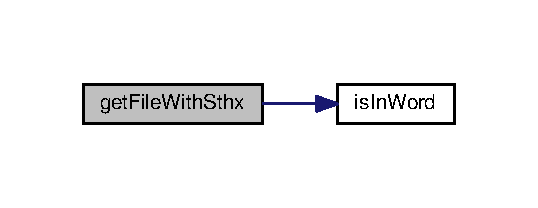
\includegraphics[width=258pt]{utilities_8h_a952a8c5f0067bb44afe28b66fdfa555b_cgraph}
\end{center}
\end{figure}


\hypertarget{utilities_8h_aed89159b1527605074e6ec1ddf945e69}{\index{utilities.\-h@{utilities.\-h}!get\-Word@{get\-Word}}
\index{get\-Word@{get\-Word}!utilities.h@{utilities.\-h}}
\subsubsection[{get\-Word}]{\setlength{\rightskip}{0pt plus 5cm}std\-::string get\-Word (
\begin{DoxyParamCaption}
\item[{{\bf ushort}}]{word\-\_\-num, }
\item[{std\-::string \&}]{chaine}
\end{DoxyParamCaption}
)}}\label{utilities_8h_aed89159b1527605074e6ec1ddf945e69}


Donne le mot n°{\itshape word\-\_\-num} dans la chaine chaine, à noter que word\-\_\-num commence par 0;. 

\hypertarget{utilities_8h_af701e0ba40a65bfd641a06968095fa75}{\index{utilities.\-h@{utilities.\-h}!is\-In\-Word@{is\-In\-Word}}
\index{is\-In\-Word@{is\-In\-Word}!utilities.h@{utilities.\-h}}
\subsubsection[{is\-In\-Word}]{\setlength{\rightskip}{0pt plus 5cm}bool is\-In\-Word (
\begin{DoxyParamCaption}
\item[{std\-::string}]{word, }
\item[{std\-::string}]{sub\-Word}
\end{DoxyParamCaption}
)}}\label{utilities_8h_af701e0ba40a65bfd641a06968095fa75}
\begin{DoxyReturn}{Returns}
true si {\itshape sub\-Word} est dans {\itshape word} 
\end{DoxyReturn}


Definition at line 59 of file utilities.\-cpp.



Referenced by get\-File\-With\-Sthx().

\hypertarget{utilities_8h_a21d81ae15fd90d0f392e4104be872296}{\index{utilities.\-h@{utilities.\-h}!positif@{positif}}
\index{positif@{positif}!utilities.h@{utilities.\-h}}
\subsubsection[{positif}]{\setlength{\rightskip}{0pt plus 5cm}float positif (
\begin{DoxyParamCaption}
\item[{int}]{a}
\end{DoxyParamCaption}
)}}\label{utilities_8h_a21d81ae15fd90d0f392e4104be872296}


Renvoie le nombre en positif. 



Definition at line 105 of file utilities.\-cpp.

\hypertarget{utilities_8h_a06369ea5ee0568ca16b620f8faa80685}{\index{utilities.\-h@{utilities.\-h}!probability@{probability}}
\index{probability@{probability}!utilities.h@{utilities.\-h}}
\subsubsection[{probability}]{\setlength{\rightskip}{0pt plus 5cm}bool probability (
\begin{DoxyParamCaption}
\item[{int}]{prob, }
\item[{int}]{sur}
\end{DoxyParamCaption}
)}}\label{utilities_8h_a06369ea5ee0568ca16b620f8faa80685}


Permet de tester une certaine probabilité 



Definition at line 35 of file utilities.\-cpp.


\hypertarget{entity_8cpp}{\section{src/\-Graphics/entity.cpp File Reference}
\label{entity_8cpp}\index{src/\-Graphics/entity.\-cpp@{src/\-Graphics/entity.\-cpp}}
}
{\ttfamily \#include \char`\"{}entity.\-h\char`\"{}}\\*
{\ttfamily \#include \char`\"{}ntsa.\-h\char`\"{}}\\*
Include dependency graph for entity.\-cpp\-:\nopagebreak
\begin{figure}[H]
\begin{center}
\leavevmode
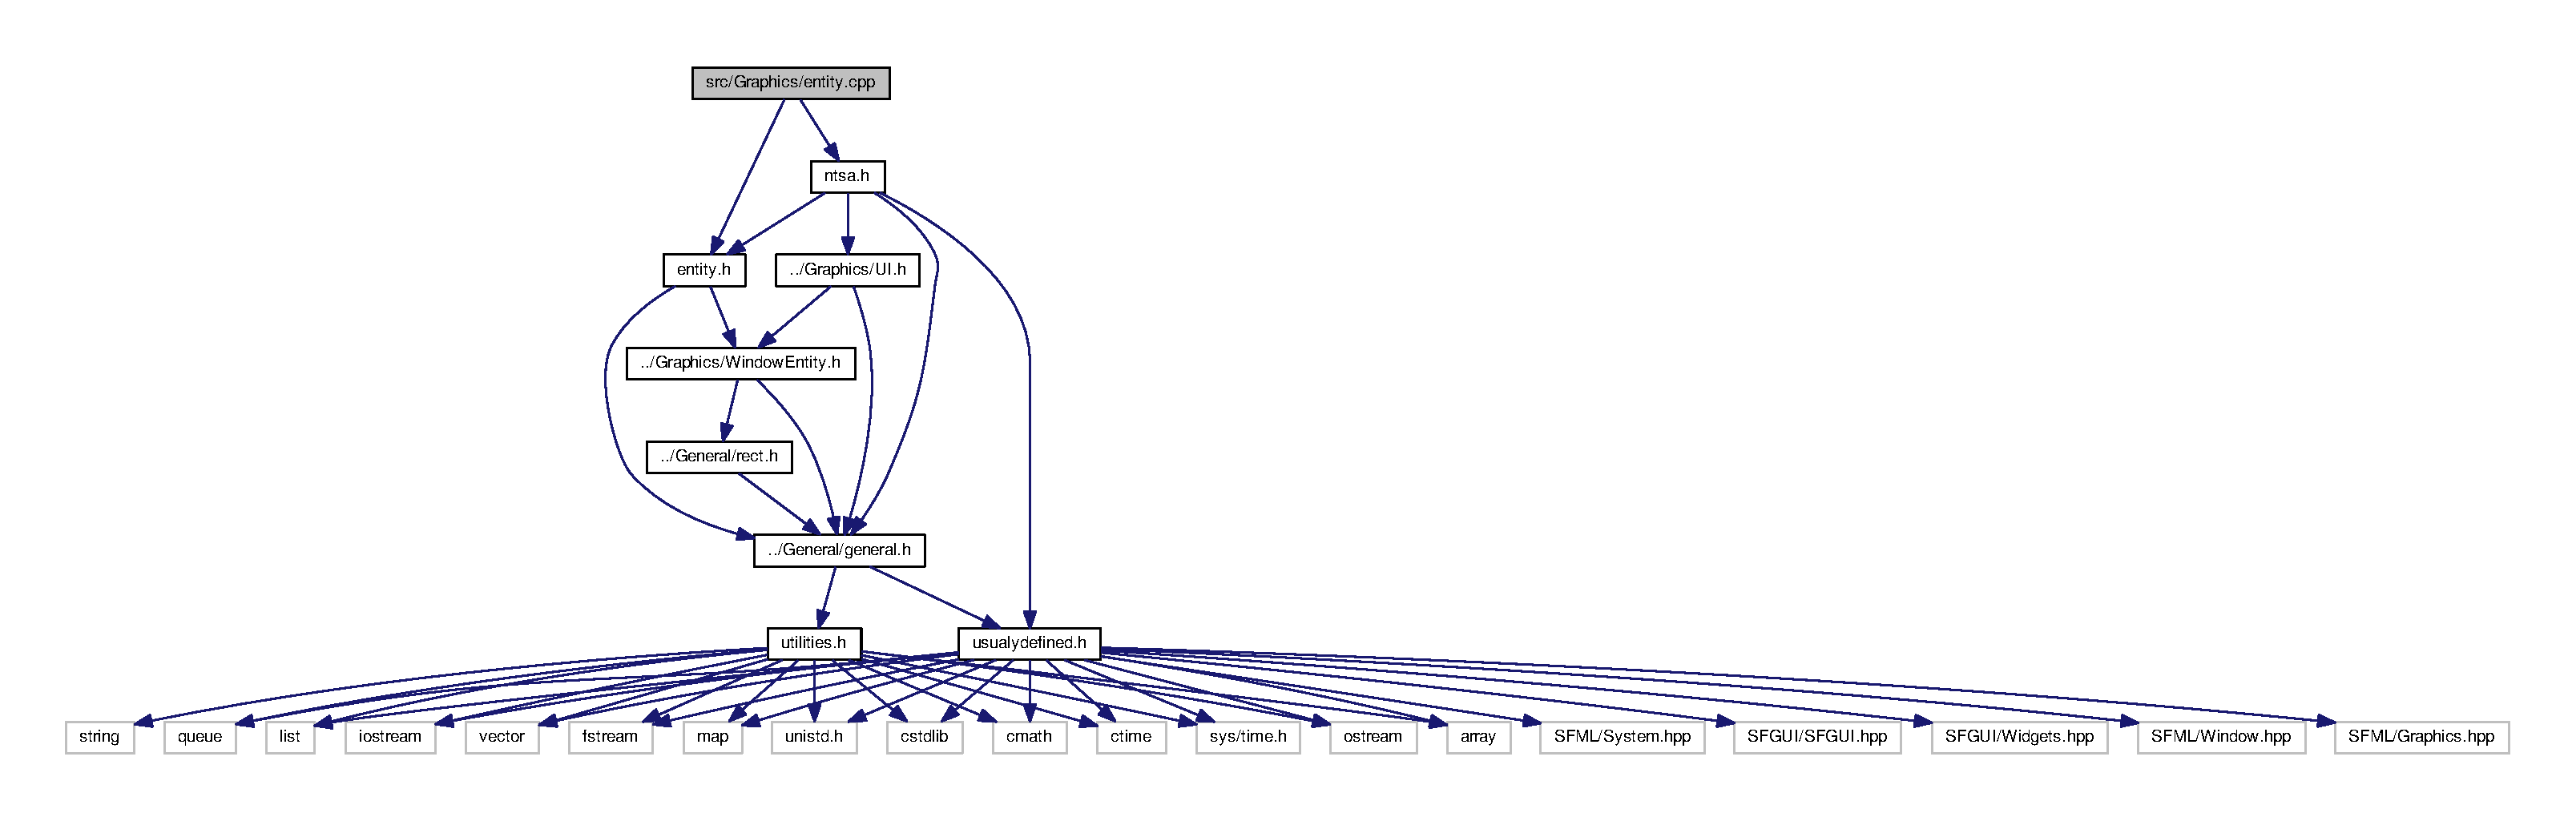
\includegraphics[width=350pt]{entity_8cpp__incl}
\end{center}
\end{figure}
\subsection*{Macros}
\begin{DoxyCompactItemize}
\item 
\#define \hyperlink{entity_8cpp_a0b40690e1be9419c96678684a0ddc609}{P\-L\-A\-Y\-E\-R\-\_\-\-S\-T\-E\-P\-\_\-\-M\-S}~20
\item 
\#define \hyperlink{entity_8cpp_ab11b9715075aa0006e714adc19c2bbd9}{P\-L\-A\-Y\-E\-R\-\_\-\-L\-I\-M\-I\-T\-\_\-\-S\-P\-E\-E\-D}~100
\end{DoxyCompactItemize}


\subsection{Macro Definition Documentation}
\hypertarget{entity_8cpp_ab11b9715075aa0006e714adc19c2bbd9}{\index{entity.\-cpp@{entity.\-cpp}!P\-L\-A\-Y\-E\-R\-\_\-\-L\-I\-M\-I\-T\-\_\-\-S\-P\-E\-E\-D@{P\-L\-A\-Y\-E\-R\-\_\-\-L\-I\-M\-I\-T\-\_\-\-S\-P\-E\-E\-D}}
\index{P\-L\-A\-Y\-E\-R\-\_\-\-L\-I\-M\-I\-T\-\_\-\-S\-P\-E\-E\-D@{P\-L\-A\-Y\-E\-R\-\_\-\-L\-I\-M\-I\-T\-\_\-\-S\-P\-E\-E\-D}!entity.cpp@{entity.\-cpp}}
\subsubsection[{P\-L\-A\-Y\-E\-R\-\_\-\-L\-I\-M\-I\-T\-\_\-\-S\-P\-E\-E\-D}]{\setlength{\rightskip}{0pt plus 5cm}\#define P\-L\-A\-Y\-E\-R\-\_\-\-L\-I\-M\-I\-T\-\_\-\-S\-P\-E\-E\-D~100}}\label{entity_8cpp_ab11b9715075aa0006e714adc19c2bbd9}


Definition at line 5 of file entity.\-cpp.



Referenced by Player\-::actualiser().

\hypertarget{entity_8cpp_a0b40690e1be9419c96678684a0ddc609}{\index{entity.\-cpp@{entity.\-cpp}!P\-L\-A\-Y\-E\-R\-\_\-\-S\-T\-E\-P\-\_\-\-M\-S@{P\-L\-A\-Y\-E\-R\-\_\-\-S\-T\-E\-P\-\_\-\-M\-S}}
\index{P\-L\-A\-Y\-E\-R\-\_\-\-S\-T\-E\-P\-\_\-\-M\-S@{P\-L\-A\-Y\-E\-R\-\_\-\-S\-T\-E\-P\-\_\-\-M\-S}!entity.cpp@{entity.\-cpp}}
\subsubsection[{P\-L\-A\-Y\-E\-R\-\_\-\-S\-T\-E\-P\-\_\-\-M\-S}]{\setlength{\rightskip}{0pt plus 5cm}\#define P\-L\-A\-Y\-E\-R\-\_\-\-S\-T\-E\-P\-\_\-\-M\-S~20}}\label{entity_8cpp_a0b40690e1be9419c96678684a0ddc609}


Definition at line 4 of file entity.\-cpp.



Referenced by Player\-::actualiser().


\hypertarget{entity_8h}{\section{src/\-Graphics/entity.h File Reference}
\label{entity_8h}\index{src/\-Graphics/entity.\-h@{src/\-Graphics/entity.\-h}}
}
{\ttfamily \#include \char`\"{}../\-General/general.\-h\char`\"{}}\\*
{\ttfamily \#include \char`\"{}../\-Graphics/\-Window\-Entity.\-h\char`\"{}}\\*
Include dependency graph for entity.\-h\-:\nopagebreak
\begin{figure}[H]
\begin{center}
\leavevmode
\includegraphics[width=350pt]{entity_8h__incl}
\end{center}
\end{figure}
This graph shows which files directly or indirectly include this file\-:\nopagebreak
\begin{figure}[H]
\begin{center}
\leavevmode
\includegraphics[width=350pt]{entity_8h__dep__incl}
\end{center}
\end{figure}
\subsection*{Data Structures}
\begin{DoxyCompactItemize}
\item 
class \hyperlink{class_space_laser}{Space\-Laser}
\begin{DoxyCompactList}\small\item\em Cette classe ressemble en tout points à \hyperlink{class_visual_effect}{Visual\-Effect} mis à part un construxteur légèrement différent. \end{DoxyCompactList}\item 
class \hyperlink{class_entity}{Entity}
\item 
class \hyperlink{class_player}{Player}
\end{DoxyCompactItemize}

\hypertarget{ntsa_8cpp}{\section{src/\-Graphics/ntsa.cpp File Reference}
\label{ntsa_8cpp}\index{src/\-Graphics/ntsa.\-cpp@{src/\-Graphics/ntsa.\-cpp}}
}
{\ttfamily \#include \char`\"{}ntsa.\-h\char`\"{}}\\*
Include dependency graph for ntsa.\-cpp\-:\nopagebreak
\begin{figure}[H]
\begin{center}
\leavevmode
\includegraphics[width=350pt]{ntsa_8cpp__incl}
\end{center}
\end{figure}

\hypertarget{ntsa_8h}{\section{src/\-Graphics/ntsa.h File Reference}
\label{ntsa_8h}\index{src/\-Graphics/ntsa.\-h@{src/\-Graphics/ntsa.\-h}}
}
{\ttfamily \#include \char`\"{}../\-General/usualydefined.\-h\char`\"{}}\\*
{\ttfamily \#include \char`\"{}../\-General/general.\-h\char`\"{}}\\*
{\ttfamily \#include \char`\"{}../\-Graphics/\-U\-I.\-h\char`\"{}}\\*
{\ttfamily \#include \char`\"{}entity.\-h\char`\"{}}\\*
Include dependency graph for ntsa.\-h\-:\nopagebreak
\begin{figure}[H]
\begin{center}
\leavevmode
\includegraphics[width=350pt]{ntsa_8h__incl}
\end{center}
\end{figure}
This graph shows which files directly or indirectly include this file\-:
\nopagebreak
\begin{figure}[H]
\begin{center}
\leavevmode
\includegraphics[width=350pt]{ntsa_8h__dep__incl}
\end{center}
\end{figure}
\subsection*{Data Structures}
\begin{DoxyCompactItemize}
\item 
class \hyperlink{class_ntsa_window}{Ntsa\-Window}
\end{DoxyCompactItemize}

\hypertarget{_window_entity_8cpp}{\section{src/\-Graphics/\-Window\-Entity.cpp File Reference}
\label{_window_entity_8cpp}\index{src/\-Graphics/\-Window\-Entity.\-cpp@{src/\-Graphics/\-Window\-Entity.\-cpp}}
}
{\ttfamily \#include \char`\"{}Window\-Entity.\-h\char`\"{}}\\*
Include dependency graph for Window\-Entity.\-cpp\-:\nopagebreak
\begin{figure}[H]
\begin{center}
\leavevmode
\includegraphics[width=350pt]{_window_entity_8cpp__incl}
\end{center}
\end{figure}

\hypertarget{_window_entity_8h}{\section{src/\-Graphics/\-Window\-Entity.h File Reference}
\label{_window_entity_8h}\index{src/\-Graphics/\-Window\-Entity.\-h@{src/\-Graphics/\-Window\-Entity.\-h}}
}
{\ttfamily \#include \char`\"{}../\-General/general.\-h\char`\"{}}\\*
{\ttfamily \#include \char`\"{}../\-General/rect.\-h\char`\"{}}\\*
Include dependency graph for Window\-Entity.\-h\-:\nopagebreak
\begin{figure}[H]
\begin{center}
\leavevmode
\includegraphics[width=350pt]{_window_entity_8h__incl}
\end{center}
\end{figure}
This graph shows which files directly or indirectly include this file\-:
\nopagebreak
\begin{figure}[H]
\begin{center}
\leavevmode
\includegraphics[width=350pt]{_window_entity_8h__dep__incl}
\end{center}
\end{figure}
\subsection*{Data Structures}
\begin{DoxyCompactItemize}
\item 
class \hyperlink{class_window_entity}{Window\-Entity}
\item 
class \hyperlink{class_visual_effect}{Visual\-Effect}
\begin{DoxyCompactList}\small\item\em Une classe gérant effet visuel temporaire. \end{DoxyCompactList}\end{DoxyCompactItemize}

\input{_p_world_gen_8cpp}
%--- End generated contents ---

% Index
\newpage
\phantomsection
\addcontentsline{toc}{chapter}{Index}
\printindex

\end{document}
